%Preamble
\documentclass[12pt]{article}   
\usepackage[
    a4paper,
    left=3.0cm,
    right=3.0cm,
    top=2.0cm,
    bottom=2.5cm]{geometry}
\usepackage{mathptmx}
\usepackage{url}
\usepackage{amsfonts}
\usepackage[fleqn]{amsmath}
\usepackage{amssymb}
\usepackage{mathtools}
\usepackage{amsthm}
\usepackage{graphicx, import}
\usepackage{listings}
\usepackage{booktabs}
\usepackage{caption}
\usepackage{calc}
\usepackage{array, multirow}
\usepackage[utf8]{inputenc}
\usepackage{csquotes}
\usepackage{color}
\usepackage{float}
\usepackage{appendix}
\usepackage[english]{babel}
\usepackage[
    backend=biber,
    style=authoryear,
    sorting=nyt]{biblatex}
\usepackage{caption}
\usepackage{titling}
\captionsetup{width=.6\textwidth}
\makeatletter
\addbibresource{bottom/refs.bib}
\addbibresource{bottom/figures.bib}
\newrobustcmd*{\parentexttrack}[1]{%
    \begingroup
    \blx@blxinit
    \blx@setsfcodes
    \blx@bibopenparen#1
    \blx@bibcloseparen
    \endgroup}
\makeatother
\usepackage{titlesec}
\usepackage{fancyhdr}
\pagestyle{fancy}
\setlength{\headheight}{15pt}
\fancyhead[L]{\leftmark}
\fancyhead[R]{}

% Biblatex url formatting
\setcounter{biburllcpenalty}{100}
\setcounter{biburlucpenalty}{200}
\setcounter{biburlnumpenalty}{100}

% Adding a forth layer of roman numeral 
\setcounter{secnumdepth}{4}
\setcounter{tocdepth}{4}
\titleformat{\paragraph}
{\normalfont\normalsize\bfseries}{\theparagraph}{1em}{}
\titlespacing*{\paragraph}
{0pt}{3.25ex plus 1ex minus .2ex}{1.5ex plus .2ex}

\AtEveryCite{%
    \let\parentext=\parentexttrack%
    %\let\bibopenparen=\bibopenbracket%
    %\let\bibcloseparen=\bibclosebracket
}
    
\newcommand{\executeiffilenewer}[3]{%
\ifnum\pdfstrcmp{\pdffilemoddate{#1}}%
{\pdffilemoddate{#2}}>0%
{\immediate\write18{#3}}\fi%
}

\newcommand{\vectorimage}[1]{
    \def\svgwidth{5.5in}
    \import{figures/}{#1.pdf_tex}
}
    
\lstset{
    basicstyle=\tiny,
    showstringspaces=false,
    tabsize=4}

\newcommand{\codeExample}[4]{
    \begin{center}\begin{tabular}{|p{1.05\textwidth}|}
    \hline
    \lstinputlisting[language=#2]{#1}\\[1pt]
    \hline
    \end{tabular}
    \captionof{figure}{#4}\label{#3}
    \end{center}}
    
%Text wrapped multi-column
\newcolumntype{C}[1]{>{\centering\arraybackslash}p{#1}}
    
%Disable auto-indent new paragraphs
\setlength{\parindent}{0pt}

%Contents page setup
\title{Automatic music transcription: Can Neural Networks\\ be used to analyse audio for generating\\ drum kit notation?}
\author{Daniel Topping\\dtopping256@gmail.com}
\date{May 2019}

%Document layout/content
\begin{document}
    
    \renewcommand*{\theparagraph}{\roman{paragraph}}
    \renewcommand\maketitlehooka{\null\mbox{}\vfill}
    \renewcommand\maketitlehookd{\vfill\null}
    \renewcommand*{\bigskip}{\vspace{1cm}}
    \renewcommand*{\thefootnote}{[\arabic{footnote}]}
	\pagestyle{plain}
	
	%Title page
	\begin{titlingpage}
    	\begin{Large}
    	    \begin{center}
    	        \vspace*{1cm}
        	    \textbf{University of Derby}\\
        	    \vspace{0.5cm}
        	    \textbf{Department of Electronics, Computing \& Mathematics}\\
        	    \vspace{1.5cm}
        	    \textbf{A project completed as part of the requirements for}\\
        	    \vspace{0.5cm}
        	    \textbf{BSc (Hons) Mathematics and Computer Science}\\
        	    \vspace{2cm}
        	    \textbf{entitled}\\
        	    \vspace{0.5cm}
        	    \makeatletter
        	    \textbf{\@title}\\
        	    \vspace{1.5cm}
        	    \textbf{by}\\
        	    \vspace{0.5cm}
        	    \textbf{\@author}\\
        	    \vspace{1.5cm}
        	    \textbf{\@date}
        	    \makeatother
    	    \end{center}
	    \end{Large}
	\end{titlingpage}
	
	%First page
	\setcounter{page}{1}
	\section*{Abstract}
	\addcontentsline{toc}{section}{Abstract}
	
	Currently, the way that a musician would transcribe music is manually by ear and then written up either on paper or with some notation software like Sibelius. This can take large amounts of time and can be prone to error; although currently, human experts are better at this than the state of the art Automatic Music Transcription (AMT) systems. The focus of this dissertation was on investigating the effectiveness of neural network models at recognising combinations of acoustic drum kit hits.\medskip
	
	Recordings of 5 acoustic drum kits were used for raw input data. This was then labelled, processed and went through various augmentation steps to produce a large, synthetic data set of multi-classed hit combinations. This synthetic, multi-classed data was then used to train 3 neural network models to varying degrees of success, with the assumption that the prediction behaviour of the models with synthetic data would be similar to predictions on real data.\medskip
	
	The model which was most accurate, with synthetic data, was Model B. In particular, the configuration with, one-hot encoded outputs and Kullback-Leibler divergence loss reached 83.8\% class accuracy over 10 epochs. Then, a larger, final model was made based on the design of Model B. Kullback-Leibler divergence loss didn't scale very well with larger models, so binary cross-entropy loss was used instead; since this gave a similar performance during testing. The final model reached 92.4\% overall accuracy across the 10 drum kit classes, which is nearly as good as an existing method that reached 99\% across 3 drum kit classes. 
	\newpage
	
	\section*{Acknowledgements}
	\addcontentsline{toc}{section}{Acknowledgements}
	I would like to thank Dr Dave Voorhis for supervising this dissertation, providing me with useful insight and feedback. Also, I would like to thank my mother for being patient enough to proof-read this and my family and friends for their support during my time studying.
	\newpage
	
	%Contents page
	\tableofcontents
	\addcontentsline{toc}{section}{Contents}
	
	\newpage
	\pagestyle{fancy}
	\section{Introduction}
	\subsection{Project rationale}
	AMT is the process of analysing audio data and creating a human readable interpretation of what was played over time. Currently, human experts are better at transcribing music than the best AMT systems \parencite{Benetos}; as there are many components to creating detailed transcripts and these need to be done to high accuracy. Aspects of this have been implemented successfully by \textcite{lunaverus} with their AnthemScore program. AnthemScore uses a convolutional neural network to recognise which musical notes to write for certain frequency bands and how long the note is sustained. However, it isn't perfect and allows for manual corrections to the transcripts. Furthermore, it doesn't distinguish between different instruments, this results in a composite score of all of the detected instruments being made.\medskip
	
	A drum kit is an unpitched instrument, comprised of drums and cymbals that can be played to produce polyphonic rhythms called drum beats. Each drum/cymbal will have a unique timbre and different combinations of these will produce a different overall texture of sound. This paper focused on the development of neural network models with the purpose of learning the timbre of the various parts of a drum kit. This was so that as well as being able to determine which drum-cymbal combinations were hit, it could distinguish between different techniques that were used; capturing more musicality from the audio information.\medskip
	
	The benefits of neural networks that are able to recognise timbre, are that better AMT systems can be created, which have the potential to split songs into different scores for each instrument. This can be applied to other areas in sound and music as well, such as cancelling out the sound of instruments during music production, or generating artificial instrument timbres as shown by Google DeepMind's WaveNet \parencite{Oord2016}. This demonstrates that there are plenty of commercially viable applications for similar models in this area of industry.\medskip
	
	\newpage
	\subsection{Aims \& Objectives}
	\label{sec:aim_and_obj}
	The aim of this paper was to demonstrate that neural networks can be used to help create musical notation for drum kits. \medskip
	
	Figure \ref{fig:drum_schematic}, shows most of the drums and cymbals that can feature on a drum kit. However, some are less common (such as the splash and china cymbals) so we don't have enough data to run reliable tests with them. For this reason, we will specifically look at: bass drum, the 3 tom drums, snare drum, crash cymbal, ride cymbal and hi-hat. As well as which drum/cymbal was hit, in transcription, it is often important to recognise the technique that was used. In the context of this report, we will be distinguishing between `open' and `closed' hi-hat as well as `normal' and `bell' hits of the ride cymbal when defining classes.\medskip
	
	\begin{figure}[H]
        \centering
        \fbox{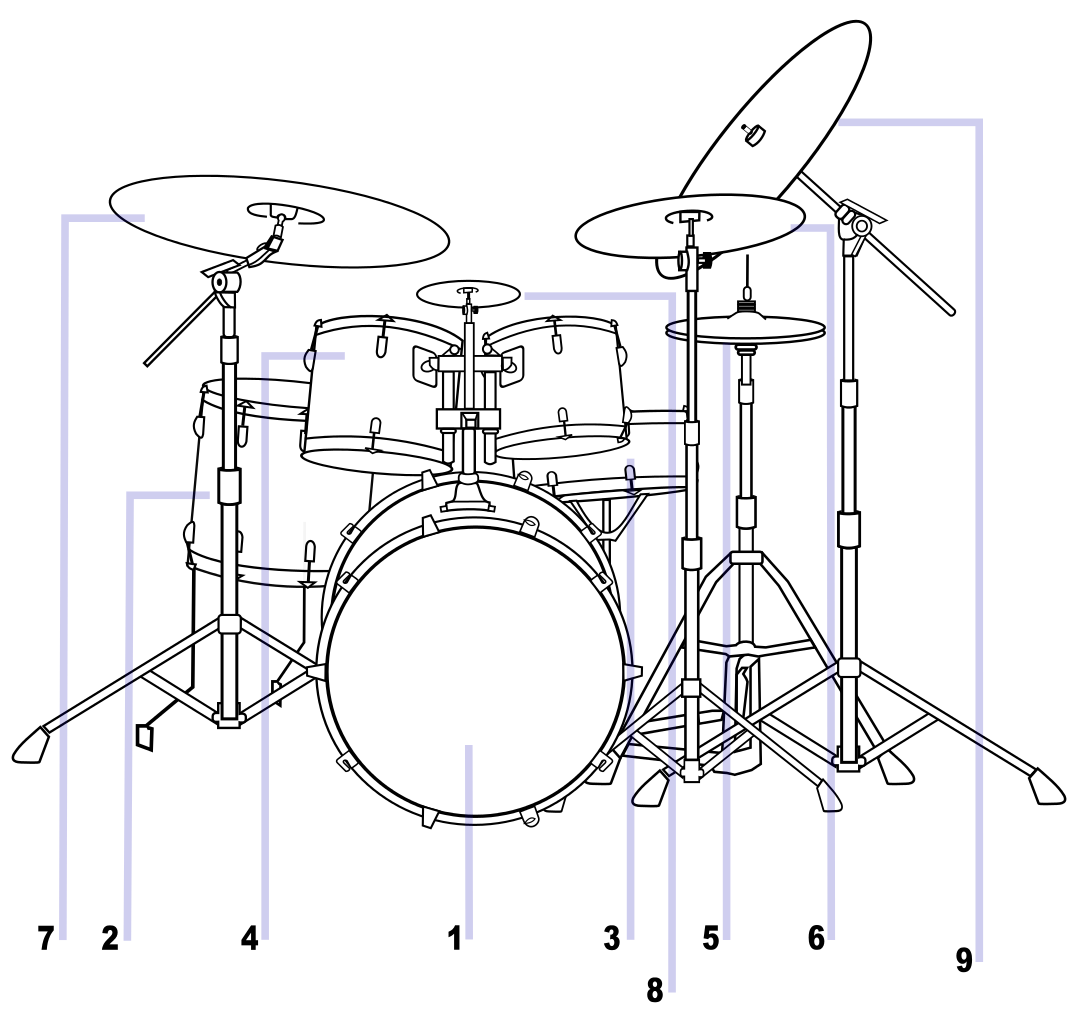
\includegraphics[width=8cm]{figures/Drums_schematic.png}}
        \caption{\footnotesize{Drum kit components: 1 - Bass drum, 2 - Low (floor) tom, 3 - Snare drum, 4 - Mid tom, 5 - Hi-hat, 6 - Crash cymbal, 7 - Ride cymbal, 8 - High tom, 9 - China cymbal. Image from \parencite{drumschematic}.}}
        \label{fig:drum_schematic}
    \end{figure}
    
    The objectives are:
    
    \begin{itemize}
	    \item Investigate different neural network models for learning drum kit timbre.
	    \item Show that differentiating timbre is a trainable feature for neural network models.
	    \item Train a neural network model to a high degree of accuracy.
	    \item Apply this model to predict drum beat sequences, with pieces of untested audio.
	\end{itemize}
	
	\newpage
	\section{Literature Review}
	\label{sec:literature_review}
    
    \setcounter{subsection}{-1}
	\subsection{Introduction}
	\label{sec:lit_review_intro}
	This literature review is split into 4 main sections: neural networks (section \ref{sec:neural_networks}); sound analysis (section \ref{sec:sound_analysis}); previous work in this area (section \ref{sec:previous_work}) and refined research questions (section \ref{sec:questions}).
	\medskip
	
	In the first section, there is a brief overview of neural networks and the back-propagation technique, as this is fundamental to the aim of this dissertation. There is a larger emphasis on convolutional neural networks because these are the current state of the art neural network models. Also, various model design patterns and structures which have been discovered during the work on GoogLeNet, ResNet and WaveNet are covered; since features of these were implemented in the design of the models used in the methodology. This section concludes with the obstacles to training machine learning models, with potential solutions to some of them.\medskip
	
	In the second section, research into various sound analysis techniques was explained, to gain some understanding of how to measure timbre and how to create audio spectrograms. Also, this section covers onset detection which was used for making scripts to automate pre-processing.\medskip
	
	In the previous work section, an alternative method of drum kit transcription using non-negative spectrogram factorisation was investigated. It was shown that this method was very reliable at detecting and classifying drum hits in polyphonic music, although it only studied 3 parts of the drum kit.\medskip
	
	The literature review finishes with some refined research questions, which will be investigated as multivariate configurations of the models in the methodology.\medskip
	
	\subsection{Neural networks}
	\label{sec:neural_networks}
	
	Artificial Neural Network (NN) models are models loosely based upon the biological processes which happen in the central nervous system of complex organisms. They are models designed to approximate a function which represents a pattern in some data \parencite{Russell;Norvig1995}. For the purpose of this report, we will use NN models for supervised learning, although there are other ways NNs can be trained.\medskip
	
	\subsubsection{Biological neurons}
	\label{sec:biological_neurons}
	
	Neurons are useful as inspiration for data processing models because each neuron performs a decision. Neurons get excited by the input from other neurons, which travel across many synapses to the neuron. If this combined excitation reaches a threshold point, then the neuron fires a signal which propagates down its axon to the synapses of other neurons. But, if it doesn't reach this threshold it doesn't fire \parencite[p.18-20]{Rojas}.\medskip
	
	\subsubsection{Artificial neurons}
	\label{sec:artificial_neurons}
	
	The behaviour of neurons has been known to have useful applications in computing since  \textcite{McCullock_Pitts} published their famous paper. They explained that the characteristics of neurons made them useful in `propositional logic', which is useful in computing because neurons can be utilised to make decisions when given data. During this time, simplistic neuron models which resembled basic logic gates were used to solve problems \parencite[p.99]{McCullock_Pitts}. However these models were quite restrictive, only using binary information as input/output and were bespoke for the problems they addressed, so they weren't reusable for slightly different problems \parencite[p.29-33]{Rojas}.\medskip
	
	\subsubsection{Perceptrons (early neuron models)}
	\label{sec:perceptron}
	
	The `Perceptron' was introduced by \textcite{Rosenblatt}. This model improved upon previous neuron models by adding weights to each input connection (see Figure \ref{fig:perceptron}). This was done because he observed that using probability theory would be a better way to investigate the brain than boolean logic \parencite[p387-388]{Rosenblatt}. This meant that learning algorithms could be used on a single perceptron, by adjusting the connection weights incrementally, to optimise towards a desirable output (see section \ref{sec:backprop_and_loss}). This could be done without having to change the overall structure as you would with McCullock-Pitts neurons. However, single perceptron models still had the downside of not being accurate when approximating problems where the decision boundary isn't linear \parencite{Raschka}. For example, the XOR problem cannot be solved by a perceptron because that problem requires the decision boundary to be of a higher order than linear \parencite[p.124-127]{Rojas}.\medskip
    
    \begin{figure}[h!]
        \centering
        \fbox{\vectorimage{perceptron}}
        \caption{This is how a perceptron works. The sum of the products of the input values and their respective weights are put through an activation function, the result is the output. It is conventional to pass $1$ into the first input $x_0$, along with the variable inputs so that the perceptron can still produce a non-zero output when the variable inputs are zero. The weight $w_0$ is called the bias.}
        \label{fig:perceptron}
    \end{figure}
    
    \subsubsection{Activation functions}
    \label{sec:activation_functions}
    
    Activation functions, which can be linear or non-linear, map the sum of the input signals (which have a linear domain) to some range \parencite{Nwankpa2018}. Non-linear activation functions are crucial to neuron models because otherwise, they would only be capable of producing linear output, which restricts the usefulness of the model \parencite[p.567-568]{Russell;Norvig1995}.\medskip
    
    There are many types of non-linear functions which can be used as activation functions. More recently, there are 3 groups of activation functions that are widely used: Sigmoid, hyperbolic and rectified linear units (ReLU) \parencite{Nwankpa2018}. ReLU functions were found to perform well for NN models built for audio, in particular, Leaky ReLU which is a variation of ReLU where the function has a slight positive gradient for the negative part of the x-axis instead of being 0 as with regular ReLU \parencite{Maas2013}.\medskip
    
    \subsubsection{Back-propagation, loss functions and initial weights}
	\label{sec:backprop_and_loss}
	
	The back-propagation algorithm adjusts weights of the inputs for each neuron incrementally so that the error (loss) is minimised. A loss function is a continuous function of the error between a prediction output of the model and the expected output that represents the actual class. This must be continuously differentiable so that optimisation algorithms such as gradient descent can minimise the loss function \parencite[p.580-581]{Russell;Norvig1995}.\medskip
	
	Two functions which can be used as loss functions are binary cross-entropy (BCE) and Kullback-Leibler divergence (KLD) which originate from information theory \parencite[p.34, p.67]{MacKay2013}. Research has indicated that the initial weights of neural network models has an affect on the overall effectiveness of learning. For models using hyperbolic activations, \textcite{Glorot2010} inspired `Glorot normal' distributions for selecting initial weights. Similarly, for ReLU activations, \textcite{HeNorm2015} inspired the `He normal' distributions for selecting initial weights. These loss functions and weight initialisers are provided by the \textcite{Keras} library.\medskip
	
	\subsubsection{Neural networks}
	\label{sec:neural_networks2}
	
	NN models contain multiple neurons which are interconnected, to create more complexity. These are capable of understanding more sophisticated patterns than single neuron models. In dense (fully-connected) NNs, each neuron in a layer is connected to each neuron in the next layer. Dense NNs are good when modelling problems where the optimal structure is unknown because over time the network will eliminate unused connections by reducing the connection weights to 0. However, although these networks can be largely successful, they tend to be resource intensive; containing large amounts of unnecessary weights.\medskip
	
	Sparse NNs are structured to improve performance by removing many connections which are assumed to have a negligible contribution to the model.\medskip
	
	\subsubsection{Convolutional neural networks}
	\label{sec:cnns}
	Convolutional Neural Network (CNN) models are neural networks which came about after \textcite{Hubel1959} did their work on the visual cortex of cats. This work inspired a structural design of neural networks where neurons only took inputs from small regions of data, making them more sparse and temporal. Also, it was observed that cats have areas in their vision that are sensitive to light as well as areas that are desensitised, allowing certain features to be picked up such as edges \parencite[p574]{Hubel1959}. CNN models use regions that use the same group of weights called `kernels' to store patterns, which filter features in a similar way.\medskip
	
	Convolution layers map small regions of space from the proceeding layer to the next layer. These regions are manipulated by a convolution kernel which is a transformation of the region. Convolution layers can be used to increase the feature space of the data by passing the same regions through many different convolution kernels. Convolution layers are usually interleaved by pooling (sub-sampling) layers \parencite{Lecun1998}. Pooling layers aim to simplify the data by down-scaling it in the sample space (see Figure \ref{fig:convolution_pooling}), although convolution layers with a stride of greater than 1 can be used to achieve the same thing \parencite{Springenberg2014}. A famous CNN is LeNet-5 \parencite{Lecun1998} which was used for handwritten digit recognition.\medskip
	
	\begin{figure}[h!]
	    \centering
	    \vectorimage{ConvolutionPooling}
	    \caption{This figure demonstrates how data is convoluted and then pooled. A: The convolution process transforms the data using a convolution kernel in sections. B: The pooling process scales down data using some selection method (in this case max-pooling uses the greatest value). In practice, this is done with many different kernels and CNNs use these in layers repeatedly to efficiently extract features from the input. \textit{Kingfisher picture from \parencite{convolutionpooling}}}
	    \label{fig:convolution_pooling}
	\end{figure}
	
	\subsubsection{Using more convolution layers instead of pooling layers}
	\label{sec:strided_conv}
	
	\textcite{Springenberg2014} pointed out that by only using convolution layers in CNNs, less data is lost than with the more traditional CNNs which used pooling. The fully-convolutional NN has become a more popular approach since this observation, with the down-scaling of the sample space done by using convolution layers with stride 2, instead of the typically used max-pooling layers.\medskip
	
	\subsubsection{Causal and dilated causal convolution layers}
	\label{sec:dilated_causal_conv}
	
	In images, it makes sense to assume that the inputs around a given input have some relationship to that input since the dimensionality of the input is 2 space dimensions. However, with audio data, this assumption doesn't make sense, because time is a dimension. Instead, we assume that for a given input, it only has a relationship to inputs in the past from it. This is the idea behind the causal convolutions used by Google DeepMind's state of the art WaveNet \parencite{Oord2016}, where neurons are only given inputs from up until present in the sample space. Dilated causal convolutions increase the receptive field of the neurons while using the same amount of inputs by spacing the connections between each layer \parencite{Oord2016}. Both of these layers were shown to be useful in creating sparser CNN's, which increased computational performance as well as the accuracy of the models.\medskip
	
	\subsubsection{Non-sequential NN designs}
	\label{sec:nonsequencial-nn-designs}
	
	Modern NN's can be very complex and don't follow a completely sequential design pattern. For example, GoogLeNet uses frequent branching and concatenation of different sized convolutions in its 'Inception modules'. These are used in a repeating pattern in their deep CNN \parencite{Szegedy2015}. It was also found that convolution layers with a 1x1 kernel were a good way to reduce the size of the feature space, without affecting the size of the sample space. This is used in GoogLeNet's Inception modules, before each  convolution layer with a larger kernel.\medskip
	
	Microsoft's ResNet demonstrated that when NN's get to a certain depth they can become less accurate, so proposed skip connections; which allow earlier activations to pass deeper into the NN \parencite{He2015}. This was important because before ResNet it was widely believed that the deeper the NN was, the better it performed.\medskip
	
	\subsubsection{Machine learning obstacles}
	\label{sec:machine_learning_obstacles}
	
	\paragraph{Multi-classed data}
	\label{sec:multiclassed_data}
	
	Many machine learning models are designed to use data with a single class per piece of data, with classes which are mutually exclusive. This data can easily be labelled\footnote{A marker associated with some data, which classifies it.} one label per class using a one-hot encoded output. For example, the MNIST data set has pictures of handwritten numbers with labels valued 0-9 \parencite{MNIST}. Only one of these labels is true per image since the classifier is the number that the handwritten digit represents which is a mutually exclusive classifier. However, classifying drum kit timbre means analysing sound that could contain multiple drums or cymbals simultaneously. The presence of these classes are not mutually exclusive so the data is multi-classed.\medskip
	
	There are multiple ways of encoding multi-classed data. The multi-hot method is where each class is assigned to one label, each is encoded as `on' or `off' depending upon the presence of the class. The one-hot method can also be used, in this context each label is assigned to a super-set, representing some combination of classes with only one label encoded as `on' and the rest are `off' \parencite{ghlmowyzz2017}. For drum kit classes we will see that for the 10 drum/cymbal classes, there are 87 feasible hit combinations. This means that with one-hot encoding there are 87 labels and with multi-class encoding, there are 10 labels.\medskip
	
	An activation function in the output layer needs to be used which will normalise the output so that it is within the domain of the class encodings. From the report by \textcite{ghlmowyzz2017}, it seems that the Softmax function is better suited to output with one-hot encoding and the Sigmoid function is better suited to output with multi-hot encoding. Their reasoning for this is that the sum of Softmax output is 1, so it is easier to train one-hot encoded classes with Softmax and harder to train multi-hot encoded classes. Sigmoid functions were found to perform better than the ReLU functions and hyperbolic functions for the final activation layer of a multi-hot encoded model, which was designed to predict combinations of 3 diseases using medical records \parencite{ghlmowyzz2017}.\medskip
	
	\paragraph{Underfitting, overfitting and generalisation} \label{sec:overfitting}
	As well as underfitting, where a machine learning model hasn't learnt enough from training on a data set, overfitting is also a problem. Overfitting is when the machine learning technique used to approximate some unknown model, creates an over-complicated model; which is very accurate to the training data, but not accurate to data which it hasn't encountered before  \parencite[p.143-145]{Rojas}. Optimally, models will generalise so that they can make accurate predictions on new and diverse data sets. A common regularisation technique is dropout, where random neuron connection weights are set to zero during training \parencite{Hinton2014}.\medskip
	
	\paragraph{Obtaining training data}
	\label{sec:data_augmentation}
	
	While it is possible to create a labelled data set manually, this can take large amounts of time and physical storage; especially if you want a high accuracy NN because more data is typically better. A solution to this is data augmentation \parencite{gmsw2016}, where incremental transformations can be used to create new data and reduce overfitting (see section \ref{sec:machine_learning_obstacles} part  \ref{sec:overfitting}). \textcite{gmsw2016} found that it is best to use data augmentation to create transforms in the data space (before getting processed by a NN), rather than mid-way through in the feature space. Data augmentation can be done as a part of pre-processing or on the fly during training, depending upon the restrictions of the machine.\medskip
	
	Another aspect of data collection that is particularly relevant for classification problems, is that certain classes tend to naturally occur more frequently than others. This is worse for smaller data sets because it becomes less feasible to remove the difference in data from the larger classes, as this reduces the size of the data set even more. The reason why this is a problem for NN models is that it will be less accurate at predicting classes with a smaller proportion of the input data. Synthetic Minority Over-sampling Technique (SMOTE) is a method proposed by \textcite{Chawla2002} to address the problem of imbalanced data sets.
	It involves creating new unique samples of the minority class in the same way that data augmentation creates new unique samples. It was shown that this approach improved the classification accuracy of minority classes \parencite{Chawla2002}.\medskip
	
	Another problem is, what are the correct proportions of training, validation and test data to use when testing a model? Too much validation and test data can impede the overall training of a NN, and on the other hand, too little means that the metrics which measure performance are less accurate.\medskip
	
	\subsection{Sound analysis}
	\label{sec:sound_analysis}
	Timbre is the information in a sound which indicates to the listener what is producing the sound. Usually, timbre is used to describe what instrument is producing the sound; we will use timbre to distinguish what drum or cymbal is hit and when.\medskip
	
	Timbre differs to overall pitch because one instrument can produce a C note while another can also produce a C note, however, they both sound different due to the materials and how the sound is created.\medskip
	
	Timbre also encompasses the duration's of various structures in the waveform\footnote{Defined as ``a usually graphic representation of the shape of a wave that indicates its characteristics (such as frequency and amplitude)", by \textcite{merriam-webster}.} of the sound; such as attack, decay, sustain and release, which are variables edited in sound production using music software \parencite[p.26-29]{Muller}. For the context of the drum kit, only the attack and decay phases are considered since the sustain and release will require many quick consecutive hits to produce and we're only interested in single hits over a very small amount of time.\medskip
	
	\subsubsection{Fourier transforms}
	\label{sec:fourier_transforms}
	A Fourier transform of a sound separates a complicated wave into its component frequencies. This technique is usually used to determine the note of pitched instruments such as a piano, however even though drums and cymbals are said to be unpitched, they still resonate at different frequencies to one another and this could be important in differentiating the timbres. In particular, the pattern of overtones for each component of the drum kit could be useful in distinguishing them.\medskip
	
	From work done on analysing the difference in the sound of violins by \textcite{Yokoyama2016}, it was shown using fast Fourier transforms, that playing style can also affect the overtones of the instrument. These can be used to detect playing technique as well as the instrument itself, which will be useful for the transcription of the technique for the drum kit.\medskip
	
	Fourier transforms can be done on a whole section of audio to generate a measure of frequency against magnitude for the whole segment. However sound changes over time, so to take the shape of a sound into account short-time Fourier transforms can be used to yield 2D spectrograms of the magnitude of the frequency over time \parencite[p.53]{Muller}.\medskip
	
	\subsubsection{Onset detection}
	\label{sec:onset_detection}
	Speed of music (tempo) is an important feature of transcripts, telling musicians how quickly music is playing. In the context of sound processing, onset detection enables us to evaluate the speed of a beat and gives a measure of how to break up music into parts. This will help place a drum or cymbal hit into a position in music \parencite[p.304]{Muller}.\medskip
	
	Energy based novelty is one way of finding onsets\footnote{The point in time at the start of a transient (sudden excitation of a waveform) \parencite{Bello2005, Muller}}, by using window functions to map a signal to localised energy over time and then find the log difference of this energy over time \parencite[p306-307]{Muller}. In the resulting output, noise can be ignored and the actual hits can then be selected by applying an adaptive threshold function \parencite{Bello2005}.\medskip
	
	\subsection{Work already done in the area of drum transcription}
	\label{sec:previous_work}
	\textcite{Paulus2005} used features taken from spectrograms of drum sounds and compared these with positive template spectrograms created from an average of some test data. The model had a 99\% `precision rate' for unprocessed data, although it was only used with 3 parts of a drum kit (hi-hat, snare drum and bass drum) which all sound very different and didn't attempt to classify different  technique.\medskip
	
	\subsection{Refined research questions}
	\label{sec:questions}
	Although the research has provided a much clearer picture of how to meet the objective, it also raises certain unanswered questions.\medskip
	
	\textbf{Input data format}\\
	Which format of input data is better for neural network accuracy, input data presented as 1D amplitude data over time or as 2D frequency density spectrogram data?\smallskip
	
	\textbf{Output data encoding}\\
	Is expressing the output as a multi-label (multi-hot encoded) problem or a super-class (one-hot encoded) problem, better for neural network accuracy?\smallskip  
	
	\textbf{Loss function}\\
	Which loss function is better at training the neural network? \smallskip
	
	\newpage
	\section{Methodology}
	\setcounter{subsection}{-1}
	\subsection{Introduction}
	This methodology explains the details of the implementation of the training, improvement and testing of 3 CNN models which were designed using elements of what was learned from previous work covered in the literature review (see section \ref{sec:literature_review}).\medskip
	
	The \textcite{Keras} Python library was used as a front-end to define the models, with TensorFlow doing the work on the back-end. This was done because Keras is more high-level than TensorFlow, so defining a NN is more legible and concise than using TensorFlow by itself and TensorFlow has been used by many researchers and companies as it is a powerful framework on its own. TensorBoard (which comes with the TensorFlow package), is also a useful tool as this makes logging data from TensorFlow callbacks easy and can produce detailed diagrams for the structure of the models.\medskip
	
	When designing the models, some of the techniques found in research didn't always work when applied to this use case or had to be adapted because of the constraints of the computational power available; so the design methodology was incremental.\medskip 
	
	To resolve the refined research questions (see section \ref{sec:questions}); models A and B used 1D amplitude input data and Model C used 2D spectrogram input data with the encoding of the output data and loss function being varied during training. When using one loss function to train the network, the others were used as metrics to aid in comparing the models, as well as a label specific accuracy (categorical accuracy or binary accuracy depending upon the encoding) and a class accuracy metric which can be used for all of the models.\medskip
	
	There is a large focus on how the input data was obtained in this methodology because NN models require large amounts of diverse data to work well.\medskip
	
	To summarise the whole process:	
	\begin{enumerate}
	    \item Raw wave file data was obtained and pre-processed, so that it was a consistent format for the CNN models to train upon and there was plenty of natural variation.
	    \item The amount of data was increased with data augmentation techniques and multi-class data was efficiently generated and labelled; using the assumption that training using synthetic multi-class data will produce a similar accuracy when predicting real multi-class data.
	    \item The synthetic data was then divided into training, validation and testing data sets.
	    \item The models were designed and adjusted by training them on a smaller subset of the training and validation data sets.
	    \item Then for each working model, it was trained using the full data set and values of loss, accuracy and other relevant metrics per epoch\footnote{A full run over all of the training and validation data} were saved to a log file.
	    \item The best model was improved and used to predict the drum/cymbal hits of data from a real beat and the accuracy was compared.
	\end{enumerate}
	
	\subsection{Obtaining input data}
	\subsubsection{Recording, processing and labelling}
	
	For neural networks to be effective at learning generalised patterns, we need the data set to be as diverse as possible (see section \ref{sec:machine_learning_obstacles}, part \ref{sec:overfitting}). There were 5 different drum kits which were recorded with 3 different pieces of recording equipment and 3 different players. Each of these factors had an effect on the overall sound of the drums played, adding to the diversity of the data.\medskip
	
	For each drum kit, the following was recorded:
	\begin{itemize}
	    \item \textit{Isolated hits}: Many slow repeated drum/cymbal hits in isolation (which are single-class), which were used for the development and benchmarking of the models.
	    \item \textit{Drum beats}: Drum beats with combinations of drum/cymbal hits (which are multi-class), which were used for evaluating the accuracy of the final model. 
	\end{itemize} \medskip
	
	Both categories of audio were manually converted into a single channel WAV, with just the isolated hits additionally being labelled by putting them into a sub-directory structure of the following pattern: hit type, kit type and technique type; which describe: the object used to hit the drums/cymbals, the drum or cymbal being hit and the technique used respectively (this is covered in detail in section \ref{sec:labelling_and_encoding}).\medskip 
	
    To get equal shapes of input data (as each recording device had a different sampling rate) and to reduce the size of the information for the efficiency of the augmentation process as well as the neural network, the isolated hits were re-sampled to 48kHz using a function from the SciPy package \parencite{SciPy}. It was down-sampled further, for efficiency to 3kHz and a custom onset detection function (see section \ref{sec:onset_detection}) using an energy-based novelty (EBN) window function and an adaptive threshold function (see Figure \ref{fig:energy_based_novelty}) were used to find where the drum waveforms start and the audio was cropped from the 48kHz version, into short snippets of 0.25 seconds (12000 samples). Each crop was saved separately in a compressed GZIP format, to reduce the physical storage taken up for each stage of processing.\medskip
	
	\begin{figure}[H]
        \centering
        \begin{tabular}{cc}
            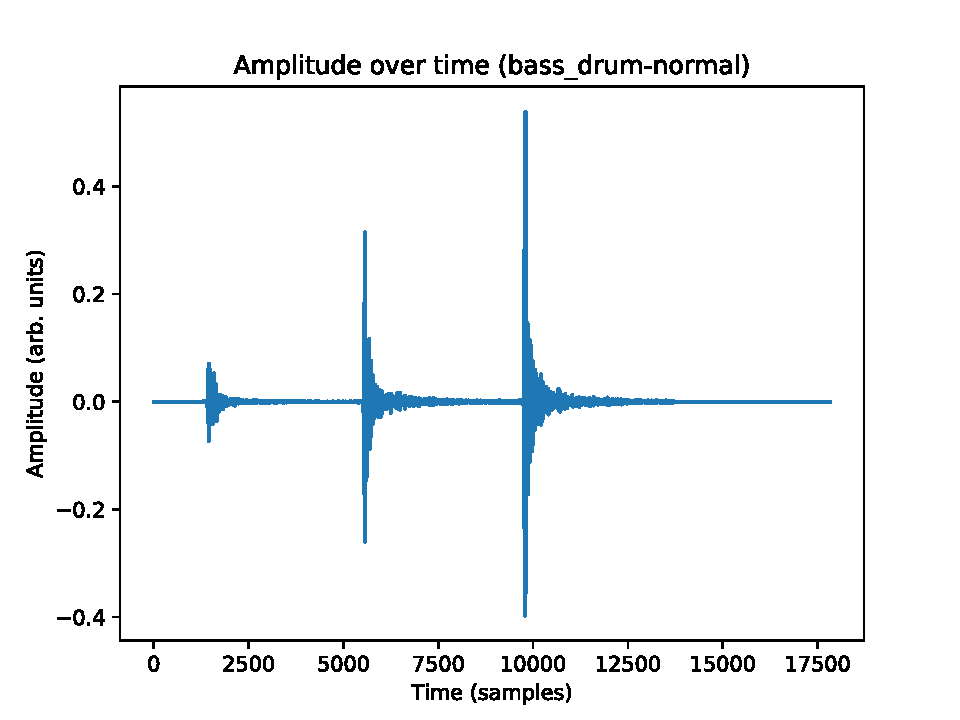
\includegraphics[width=0.4\textwidth]{figures/3_bass_drums_amplitude.pdf}&
            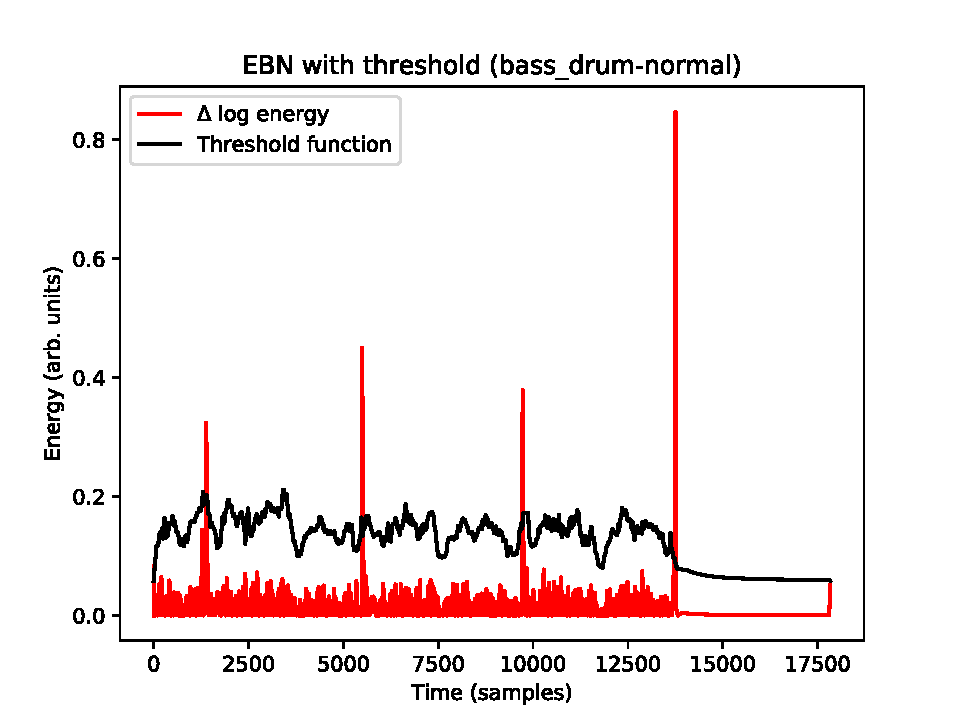
\includegraphics[width=0.4\textwidth]{figures/3_bass_drums_ebn_threshold.pdf}\\
        \end{tabular}
        \caption{\footnotesize{On the left, is the amplitude over time of a recording of 3 bass drum hits. On the right, is the EBN against an adaptive threshold function, where onsets are taken to be the first point above the threshold with an upward gradient. This method is used to detect the start of transients in audio, but will also detect unwanted transients where audio is suddenly muted (during manual processing) and will make peaks at either end due to the window function. The peak-picker identified the peaks at 1382, 5494 and 9722 which are correct, as well as, 13753 which is where the background noise is suddenly muted.}}
        \label{fig:energy_based_novelty}   
    \end{figure}
    
    \subsubsection{Data augmentation}
    \label{sec:data_augmentation_methodology}
    
    By this stage, 1069 audio segments were collected, but neural networks require a lot more data to be effective. So data augmentation (see section \ref{sec:machine_learning_obstacles} part \ref{sec:data_augmentation}) was used to create more data by transforming existing data.\medskip
	
	Data augmentation transformations were used before and after the single-class data was made into multi-class data (see Figure \ref{fig:augmentations}). These were each applied in 10 different amounts per augmentation per crop and in all possible combinations, while making sure that the sound isn't unrecognisable, ensuring that the label is still valid.\medskip
	
	\begin{figure}[H]
        \centering
        \begin{tabular}{c|c}
            Single-class augmentations & Multi-class augmentations \\
            \hline
            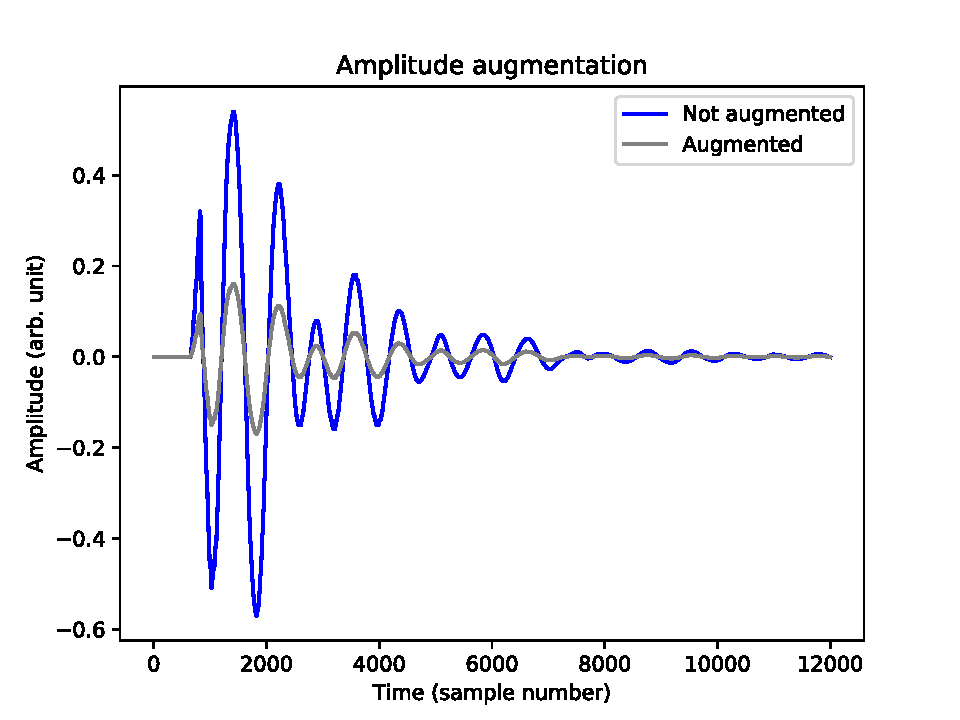
\includegraphics[width=0.35\textwidth]{figures/amplitudeAugmentation.pdf}&
            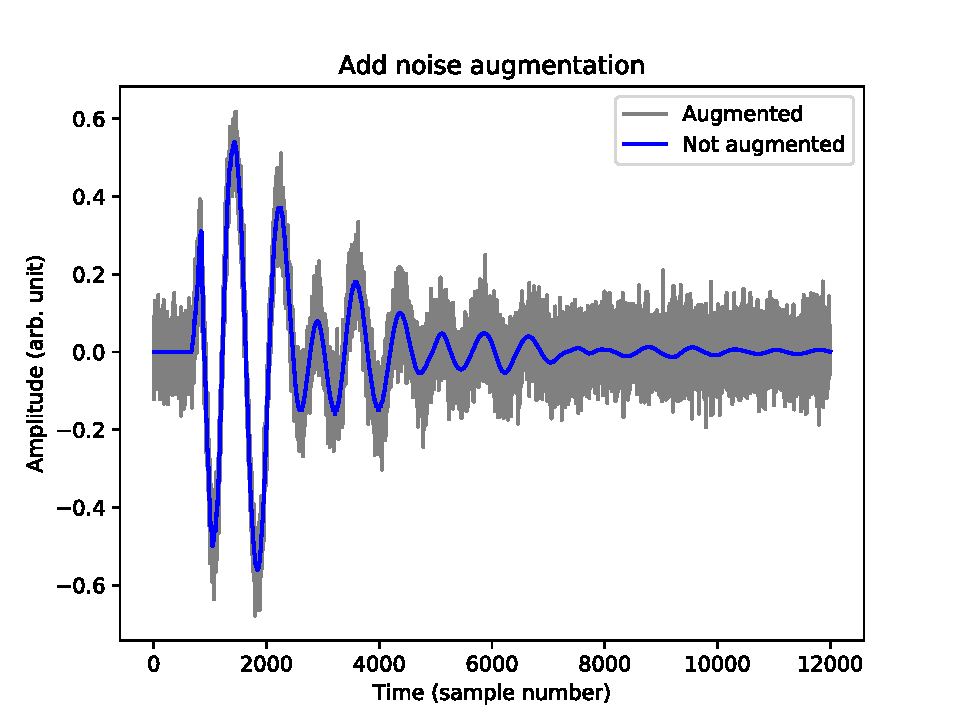
\includegraphics[width=0.35\textwidth]{figures/addNoiseAugmentation.pdf}\\
            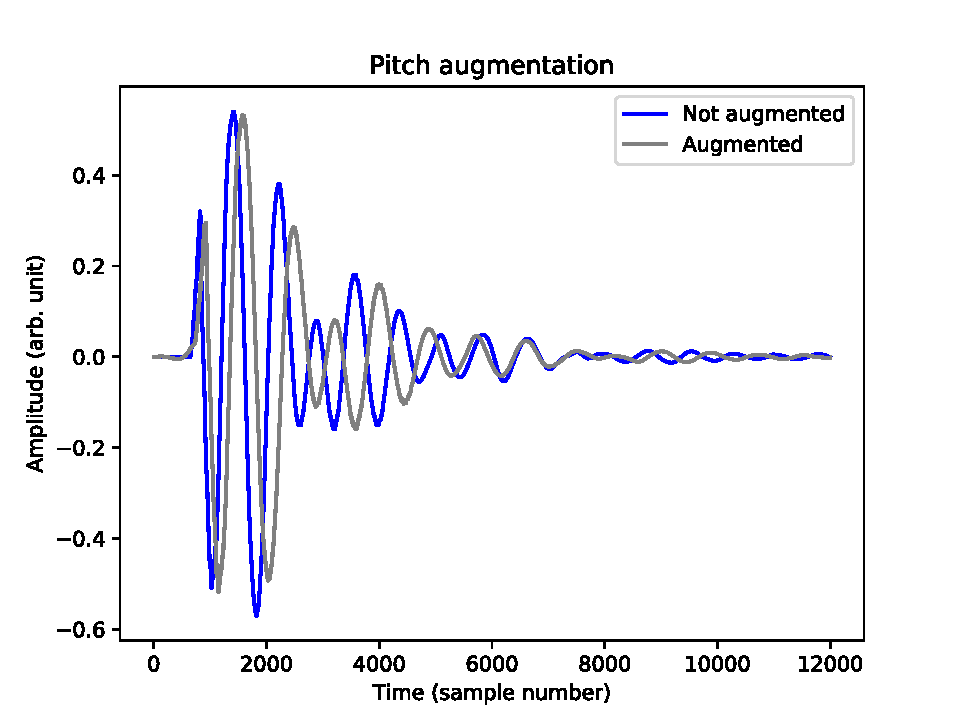
\includegraphics[width=0.35\textwidth]{figures/pitchAugmentation.pdf}&
            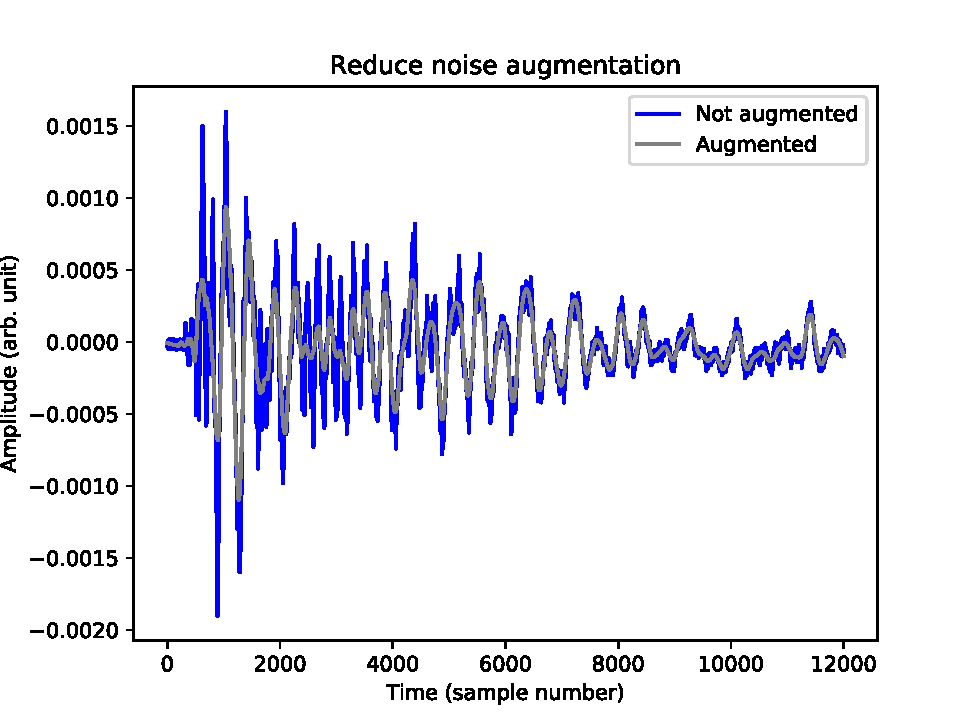
\includegraphics[width=0.35\textwidth]{figures/reduceNoiseAugmentation.pdf}\\
            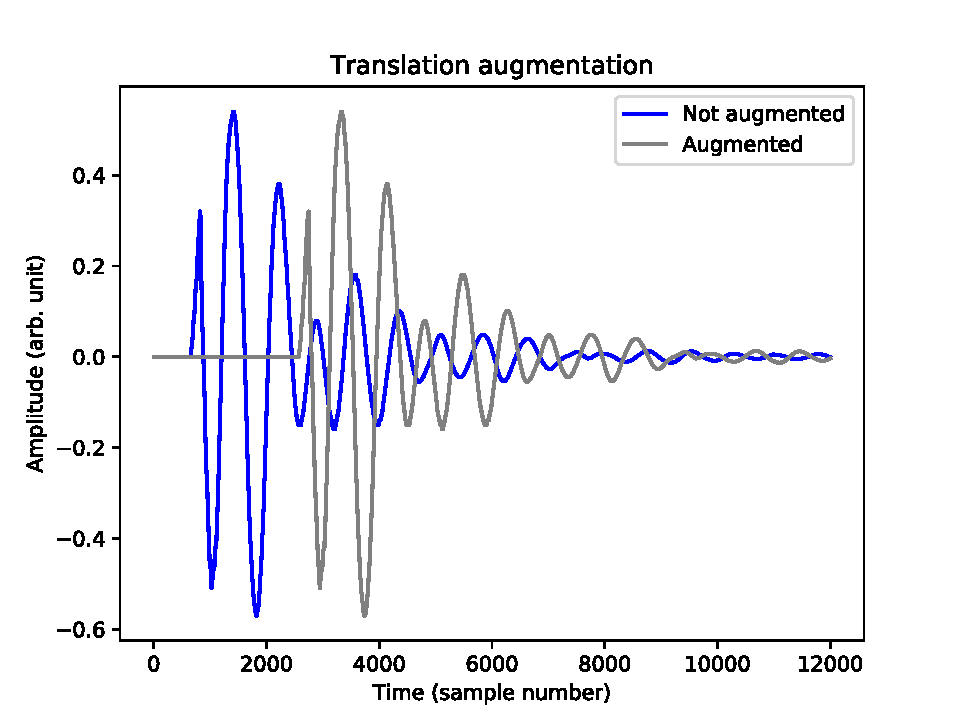
\includegraphics[width=0.35\textwidth]{figures/translationAugmentation.pdf}& \\
        \end{tabular}
    \caption{\footnotesize{Plots of the individual data augmentation transformations on bass drum waveforms. For each plot, the original waveform (in blue) is against the transformed waveform (in grey); with sample number on the x-axis and amplitude on the y-axis.}}
    \label{fig:augmentations}
    \end{figure}
    
    The single-class augmentations aim to diversify the data for how a drum or cymbal could sound. Pitch is one way of altering the sound while preserving its class. Pitch varies naturally depending on the materials used to make the instrument, the shape of the instrument, the tension of the drum skins, etc. Similarly, drums and cymbals can be played softer or louder relative to one another so the amplitude is augmented. Lastly, drums and cymbals can be played in slightly different orders since they won't occur at precisely the same time, so the translation along the time axis of the waveform is augmented. The NumPy package, included with \textcite{SciPy} and the \textcite{Librosa} package was used for transforming the data.\medskip
    
    For each valid combination of classes, augmented single-class waveforms were superimposed by taking the sum of the amplitude values together element-wise, producing multi-class data. Augmented single-class data was reused multiple times for making multi-class data, but was not used in the same combination; which guarantees that each one is unique.\medskip
    
    Here an assumption is made, that superimposing the single-class data in this way creates synthetic multi-class data that is very similar to real multi-class data. However, since two recordings can come from different places with varied sound quality and acoustics this is just an assumption. Even so, it can be observed that waveforms made this way do strongly resemble real waveforms (see Figure \ref{fig:synthetic_vs_real}).\medskip
    
    \begin{figure}[H]
        \centering
        \begin{tabular}{cc}
            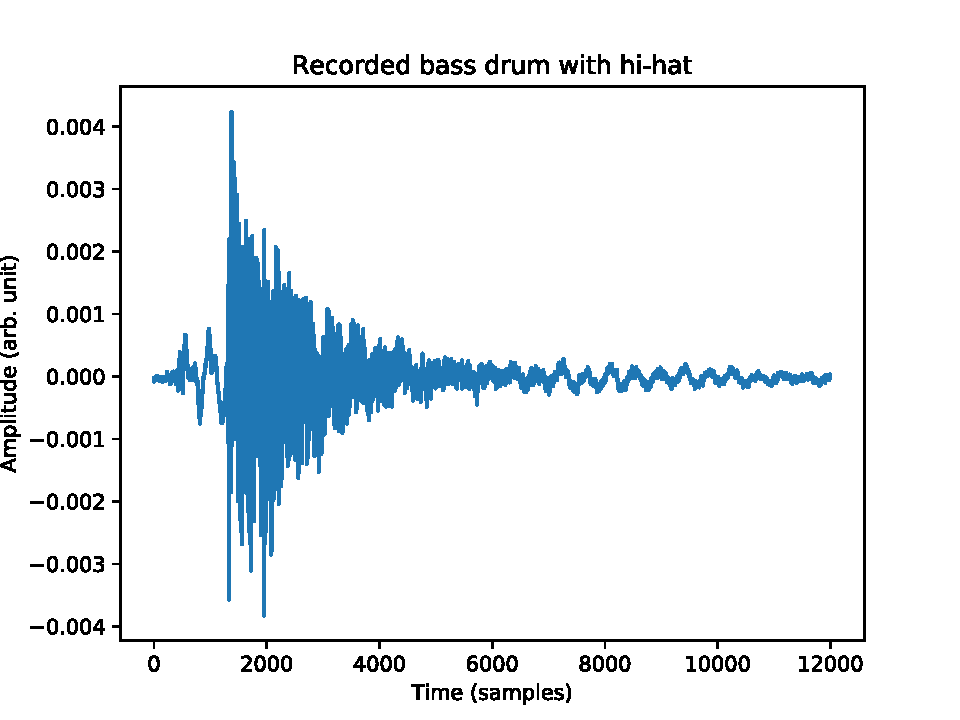
\includegraphics[width=0.35\textwidth]{figures/recorded_bd_hh.pdf}&
            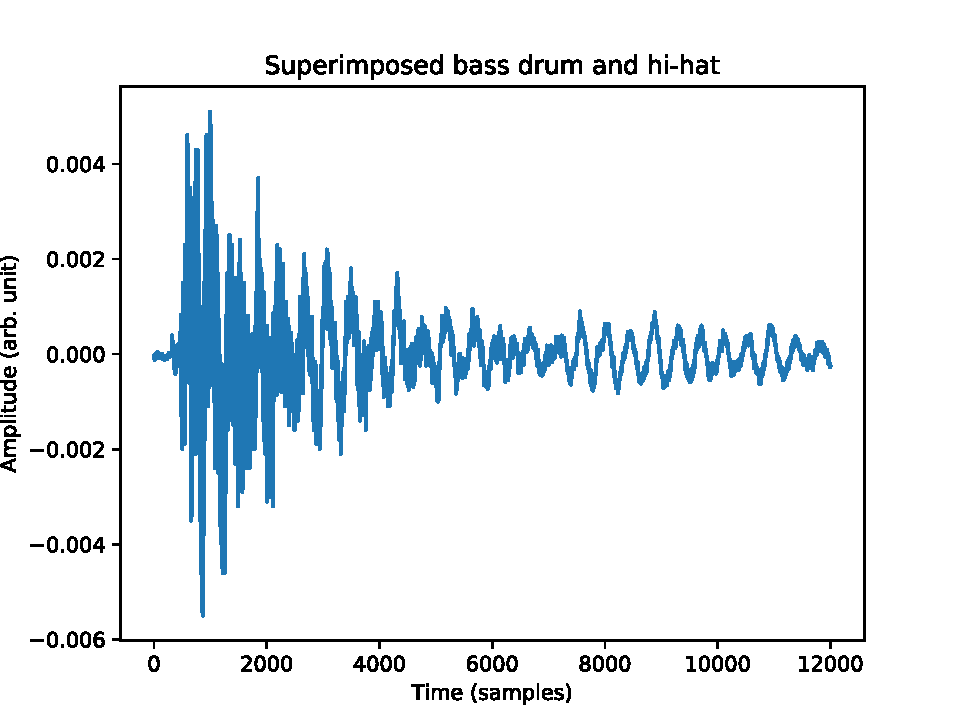
\includegraphics[width=0.35\textwidth]{figures/superimposed_bd_hh.pdf}\\
        \end{tabular}
        \caption{\footnotesize{This compares an actual recording of a bass drum and hi-hat hit together (on the left), with a superimposed bass drum and hi-hat hits which were recorded separately (on the right). As you can see the waveforms look very similar. We can see a difference in translation since the superimposed hits start together and in the actual recording, there is a lag of a fraction of a second between where the drummer plays the bass drum followed by the hi-hat. Also, there is a change in relative amplitude of bass drum and hi-hat between the graphs, as the waveform of the hi-hat is a lot more clear and less distorted by the bass drum with the recorded version than with the superimposed version.}}
        \label{fig:synthetic_vs_real}
    \end{figure}
    
    After the data is made into multi-class data, it makes sense for augmentations involving adding white noise and reducing noise to be applied uniformly. This is because noise won't vary with the instrument, but with the recording device.\medskip
    
    At the end of processing, there were in total 132,243 files that could be used for training taken from various stages of this process (see Figure \ref{fig:data_origin_table}), which is a vast improvement from 1069 at the start.\medskip
    
    \begin{figure}[H]
        \centering
        \begin{tabular}{l|l}
            Processing stage & Audio files\\
            \hline
            Single-class with no augmentation & 1069\\
            Single-class with APT augmentations & 31868\\
            Multi-class with no augmentation & 188\\
            Multi-class just APT augmentations & 8689\\
            Multi-class just noise augmentations & 2140\\
            Multi-class with all augmentations & 116760\\\bottomrule
        \end{tabular}
        \caption{\footnotesize{Number of files collected for the input data from each stage of processing. APT augmentations = amplitude-pitch-translation augmentations. Note: variants of the data were made which skipped certain steps, such as: 'multi-class with no augmentation' and 'multi-class just noise augmentations'.}}
        \label{fig:data_origin_table}
    \end{figure}
    
    \subsubsection{Labelling and encoding}
    \label{sec:labelling_and_encoding}
    To label large quantities of data efficiently, sub-directories were structured in the following way: hit types, kit types and technique types (see Appendix \ref{app:classification}). This was done so that multiple characteristics of a hit could be labelled and this would represent one class. When the data became multi-classed after isolated hits were superimposed (see section \ref{sec:data_augmentation_methodology}) these labels would merge.\medskip
    
    Classes were encoded during training, by a custom generator object which inherits from the Keras generator. This reads the labels from the audio file-path and encodes them as one-hot or multi-hot:\medskip
    
    \textbf{One-hot encoding}\\
    For this case, a matrix of size 87 (number of combinations) is produced, where the $j$\textsuperscript{th} bit is 1 and the rest are 0, with $j$ being the index of the hit combination label (see Appendix \ref{app:kit-combinations}).\medskip
    
    \textbf{Multi-hot encoding}\\
    For this case a matrix of size 10 (number of classes) is produced, where a label is 1 if the drum/cymbal class is present in the combination. Note: for valid combinations, a maximum of 3 1's will be present at any given multi-hot matrix.\medskip
    
    \subsubsection{Spectrograms}
    \label{sec:spectrograms}
    The generator object was also responsible for converting the audio into spectrograms (when necessary) in real-time. Spectrograms would be used for some of the models to compare their performance to other similar models using 1D amplitude. For creating the spectrograms, the spectrogram method of the SciPy package was used; which uses short-time Fourier transforms (see section \ref{sec:fourier_transforms}) to create 2D linear spectrogram output. It was found that to closer represent how humans hear, this could be made logarithmic; this had the effect of increasing the detail of the overtones shown but also increased the amount of noise in the spectrograms (see Figure \ref{fig:spectrograms}).\medskip
    
    \begin{figure}[H]
        \centering
        \begin{tabular}{c|c}
            Linear magnitude & Logarithmic magnitude \\
            \hline
            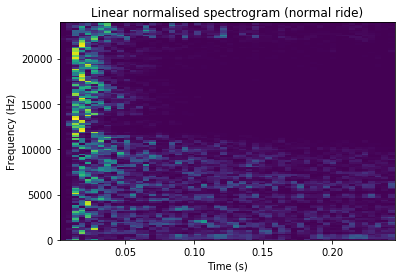
\includegraphics[width=0.45\textwidth]{figures/linear_spectrogram_ride_normal.png}&
            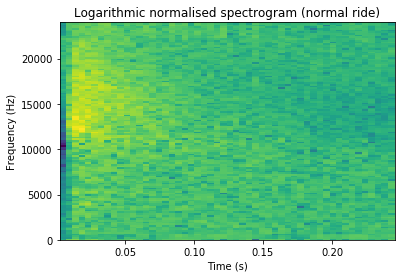
\includegraphics[width=0.45\textwidth]{figures/log_spectrogram_ride_normal.png}\\
            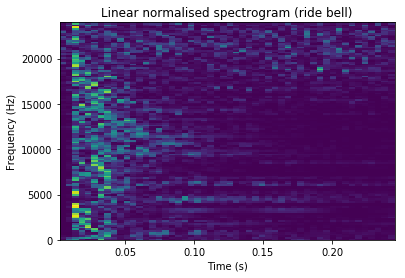
\includegraphics[width=0.45\textwidth]{figures/linear_spectrogram_ride_bell.png}&
            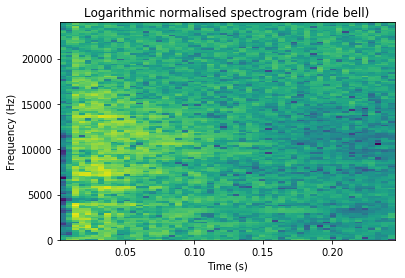
\includegraphics[width=0.45\textwidth]{figures/log_spectrogram_ride_bell.png}
        \end{tabular}
        \caption{\footnotesize{Here are the 129x53 spectra of two ride cymbal hits. All have been normalised and represent the data that is given to the 2D CNN models. Linear magnitude is much less sensitive to small changes than logarithmic magnitude. This means logarithmic magnitude suffers from having a lot of noise, however on the plus side, logarithmic magnitude exaggerates differences between timbres.}}
        \label{fig:spectrograms}
    \end{figure}
    
    \subsubsection{Dividing input data into training, validation and test data sets}
    The rationale behind dividing input data in this way is to have a measure of whether the model is underfitting, overfitting or is generalising (see section \ref{sec:machine_learning_obstacles} part \ref{sec:overfitting}). The more data allocated to training the network compared to validation and testing, the less reliable the accuracy measure is for validation and testing; however, the network needs as much training data as possible to make accurate predictions in the first place. For this reason, the data was split 3:1:1 into training, validation and testing respectively.\medskip
    
    \subsection{Model design}
    There were 3 deep CNN models designed. For simplicity, they are referred to as Model A, Model B and Model C.\medskip
    
    All of the models used the following design principles, which were covered in the literature: start with convolution layers of a stride greater-than 1, to reduce the size of the sample space (see section \ref{sec:strided_conv}); every so often use dropout layers in the structure to randomly sever network connections during training (see section \ref{sec:machine_learning_obstacles} part \ref{sec:overfitting}), which increase in drop-rate\footnote{The probability that a connection is severed by a dropout layer during training.} as dropout layers occur deeper into the network; use 1x1 convolution layers instead of pooling layers to reduce the feature space (see section \ref{sec:nonsequencial-nn-designs}), preserving detail; and at regular intervals use skip connections (see Section \ref{sec:nonsequencial-nn-designs}), so that older features have a greater effect on output.\medskip
    
    As an overview, Models A and B analyse 1-dimensional amplitude float data in the domain of -1.0 and 1.0, while Model C analyses spectrograms of the same data, made using short-time Fourier transforms (see Section \ref{sec:fourier_transforms}) with the SciPy python package. This data, in the form of spectrograms, have a different shape that is 2 dimensional instead of 1 dimensional. Model A has the largest number of layers compared to Models B and C which are similar in design except that C uses 2D convolution layers instead of 1D convolution layers. All models use skip connections, but only Model A uses inception modules (see section \ref{sec:nonsequencial-nn-designs}).\medskip
    
    Models were made so that they could be run by a machine using the `GeForce GTX 650' graphics card, this involved making sure that layer shapes were small enough to fit into less than 2GB of memory. For this reason, multiple 2 stride convolution layers were used at the start of each model, to down-scale the sample space, some models used a maximum of 32 filters and the batch size was 50. The processing speed of model training, was proportional to the number of layers in the model, that the GPU and CPU had to process. This is because each layer needs to wait for the previous layer.\medskip
    
    \subsubsection{Model A}
    \label{sec:design_modelA}
    
    This model takes 1D amplitude data in a $(B, 12000, 1)$ shape to make predictions. The batch size ($B$) used during training was 50. The shape of the output is $(B, O)$ where $O$ is 87 or 10 when the encoding is one-hot or multi-hot respectively. It makes use of causal convolution (CC), dilated CC, dropout, inception modules and skip connections. After CC layers, the Tanh hyperbolic activation function is used and for the final dense layer Softmax or Sigmoid is used as the activation function for one-hot encoding and multi-hot encoding respectively.\medskip

    \begin{figure}[H]
        \centering
        \begin{scriptsize}
            \begin{tabular}{l|l|l|l|l|l|l|l|l|}
                &\multicolumn{5}{c|}{Layers} & Activation & Matrix shape & Amount\\
                \hline
                \hline
                \multirow{5}{2cm}{Initial down-sampling layers} &\multicolumn{5}{|l|}{CC 7/8 (s = 3)} & - & $(B, 12000, 1)$ &\multirow{5}{*}{x1}\\
                \cline{2-8}
                &\multicolumn{5}{|l|}{CC 7/16 (s = 2)} & Tanh & $(B, 4000, 8)$ &\\
                \cline{2-8}
                &\multicolumn{5}{|l|}{CC 5/32 (s = 2)} & Tanh & $(B, 2000, 16)$ &\\
                \cline{2-8}
                &\multicolumn{5}{|l|}{CC 5/32 (s = 2)} & Tanh & $(B, 1000, 32)$ &\\
                \cline{2-8}
                &\multicolumn{5}{|l|}{Dropout layer (rate = 0.1)} & - & $(B, 500, 32)$ &\\
                \bottomrule
                \multirow{8}{2cm}{Inception module} &\multirow{5}{*}{Skip} & \multicolumn{4}{l|}{Dilated CC 3/32 (d = 2)} & Tanh & $(B, 500, 32)$ & \multirow{7}{*}{x3}\\
                \cline{3-8}
                & & \multirow{2}{*}{CC 1/32} & CC 1/1 & CC 1/1 & CC 1/1 & - & $(B, 500, 32)$ &\\
                \cline{4-8}
                & & & CC 3/32 & CC 5/32 & CC 7/32 & Tanh & $(B, 500, 1)$ &\\
                \cline{3-8}
                & & \multicolumn{4}{|l|}{Concat} & Tanh & $(B, 500, 128)$ &\\
                \cline{3-8}
                & & \multicolumn{4}{|l|}{CC 1/1} & Tanh & $(B, 500, 32)$ &\\
                \cline{2-8}
                & \multicolumn{5}{|l|}{Matrix addition} & - & $(B, 500, 32)$ &\\
                \cline{2-8}
                & \multicolumn{5}{|l|}{Dropout layer (rates: 0.15, 0.20, 0.25)} & - & $(B, 500, 32)$ &\\
                \bottomrule
                \multirow{3}{2cm}{Flatten and dense layers} & \multicolumn{5}{|l|}{Flattened layer} & - & $(B, 500, 32)$ & \multirow{3}{*}{x1}\\
                \cline{2-8}
                & \multicolumn{5}{|l|}{Dense layer}& Softmax or Sigmoid & $(B, 16000)$ &\\
                \cline{2-8}
                & \multicolumn{5}{|l|}{Output} & - & $(B, O)$ &\\
                \bottomrule
            \end{tabular}
        \end{scriptsize}
        \caption{\footnotesize{A tabular representation of the structure of Model A, where: CC layers denoted with `$x/y$' means $x$ kernel size by $y$ filters, `s' is the stride, `rate' is the probability of a dropped connection and `d' is the dilation rate. The matrix shape $(a, b, c)$ shows the batch size ($a$), sample space size ($b$) and the feature space size ($c$); after the flattened layer, the sample space and feature space become the same dimension ($b\times c$). Note: for CCs where the stride and dilation rate are not specified, the stride is 1 and the dilation rate is 1 (no dilation). See Appendix \ref{app:modelA_diagram} for the TensorBoard diagram.}}
        \label{fig:modelA_structure}
    \end{figure}
    
    As shown by Figure \ref{fig:modelA_structure}, Model A makes use of 4 convolution layers with a stride greater-than 1 at the beginning, which reduce the sample space from 12000 nodes to 500 while adding 32 filters to the feature space.\medskip
    
    Model A uses the hyperbolic Tanh function as its activation function between CC layers because Tanh was found to perform well with the WaveNet NN model \parencite{Oord2016}, with the weights initialised from random numbers based on the Glorot normal distribution (see section \ref{sec:backprop_and_loss}).\medskip
    
    Model A, has 3 lots of inception modules which split the activation of a 32 filter, dilated causal convolution layer into 4 distinct towers. For 3 of these towers, first, a convolution layer with a kernel size of 1 reduces the feature space to 1. This is then followed by another convolution layer with a larger kernel size (3, 5 or 7). For the other tower, a convolution layer of kernel size 1, with 32 filters is used. After this all of the towers' activations are concatenated along the feature axis which produces a layer with 128 filters and the sample space is kept the same. This is reduced back down to 32 filters by another convolution layer with a kernel size of 1 before being added to the activation from the skip connection. At the end of each module is a dropout layer which has a probability to sever connections during training, this increases from 15\% in the first module to 20\% in the second and is 25\% in the final module.\medskip
    
    After the inception modules, the CNN is flattened and put through a dense layer which has an output that is the same same as the encoded labels. The activation function throughout this model is Tanh apart from the final layer which is Softmax for one-hot encodings and Sigmoid for multi-hot encodings.
    
    \newpage
    \subsubsection{Model B}
    \label{sec:design_modelB}
    
    Like Model A, this model takes 1D amplitude data in a $(B, 12000, 1)$ shape to make predictions. The batch size ($B$) used during training was 50. Again, the shape of the output is $(B, O)$ where $O$ is 87 or 10 when the encoding is one-hot or multi-hot respectively. It makes use of CC, dilated CC, dropout and skip connections. For this model, a leaky ReLU activation function is used between CC layers and for the final dense layer Softmax or Sigmoid is used as the activation function for one-hot encoding and multi-hot encoding respectively.\medskip

    \begin{figure}[H]
        \centering
        \begin{scriptsize}
            \begin{tabular}{l|l|l|l|l|l|l|l|l|}
                &\multicolumn{5}{c|}{Layers} & Activation & Matrix shape & Amount\\
                \hline
                \hline
                \multirow{5}{2cm}{Initial down-sampling layers} &\multicolumn{5}{|l|}{CC 7/8 (s = 3)} & - & $(B, 12000, 1)$ &\multirow{5}{*}{x1}\\
                \cline{2-8}
                &\multicolumn{5}{|l|}{CC 7/16 (s = 2)} & Leaky ReLU (g = 0.3) & $(B, 4000, 8)$ &\\
                \cline{2-8}
                &\multicolumn{5}{|l|}{CC 5/32 (s = 2)} & Leaky ReLU (g = 0.3) & $(B, 2000, 16)$ &\\
                \cline{2-8}
                &\multicolumn{5}{|l|}{CC 3/32 (s = 2)} & Leaky ReLU (g = 0.3) & $(B, 1000, 32)$ &\\
                \cline{2-8}
                &\multicolumn{5}{|l|}{Dropout layer (rate = 0.1)} & - & $(B, 500, 32)$ &\\
                \bottomrule
                \multirow{5}{2cm}{Stacked dilated CC layers} &\multirow{3}{*}{Skip} & \multicolumn{4}{l|}{CC 1/1} & - & $(B, 500, 32)$ & \multirow{5}{*}{x3}\\
                \cline{3-8}
                & & \multicolumn{4}{l|}{Dilated CC 3/8 (d = 2)} & - & $(B, 500, 1)$ &\\
                \cline{3-8}
                & &\multicolumn{4}{l|}{Dilated CC 3/32 (d = 2)} & Leaky ReLU (g = 0.3) & $(B, 500, 8)$ &\\
                \cline{2-8}
                & \multicolumn{5}{|l|}{Matrix addition} & - & $(B, 500, 32)$ &\\
                \cline{2-8}
                & \multicolumn{5}{|l|}{Dropout layer (rates: 0.15, 0.20, 0.25)} & - & $(B, 500, 32)$ &\\
                \bottomrule
                \multirow{3}{2cm}{Flatten and dense layers} & \multicolumn{5}{|l|}{Flattened layer} & - & $(B, 500, 32)$ & \multirow{3}{*}{x1}\\
                \cline{2-8}
                & \multicolumn{5}{|l|}{Dense layer}& Softmax or Sigmoid & $(B, 16000)$ &\\
                \cline{2-8}
                & \multicolumn{5}{|l|}{Output} & - & $(B, O)$ &\\
                \bottomrule
            \end{tabular}
        \end{scriptsize}
        \caption{\footnotesize{A tabular representation of the structure of Model B, where: CC layers denoted with `$x/y$' means $x$ kernel size by $y$ filters, `s' is the stride, `rate' is the probability of a dropped connection, `d' is the dilation rate and `g' is the gradient of the negative part of the Leaky ReLU activation function. The matrix shape $(a, b, c)$ shows the batch size ($a$), sample space size ($b$) and the feature space size ($c$); after the flattened layer, the sample space and feature space become the same dimension ($b\times c$). Note: for CCs where the stride and dilation rate are not specified, the stride is 1 and the dilation rate is 1 (no dilation). See Appendix \ref{app:modelB_diagram} for the TensorBoard diagram.}}
        \label{fig:modelB_structure}
    \end{figure}
    
    As shown by Figure \ref{fig:modelB_structure}, Model B makes use of 4 convolution layers with a stride greater-than 1 at the beginning, which reduce the sample space from 12000 nodes to 500 while adding 32 filters to the feature space.\medskip
    
    Model B uses Leaky ReLU (see section \ref{sec:activation_functions}) as an activation function between layers. The gradient of the negative part of Leaky ReLU was set to 0.3. The weights were initialised from random numbers based on the He normal distribution (see section \ref{sec:backprop_and_loss}).\medskip
    
    Model B has 3 lots of sections which contain stacked dilated CC layers. This section starts with a causal convolution layer with a kernel size of 1 and 1 filter to reduce the feature space. Then this is followed by 2 consecutive dilated CC layers which are dilated at a rate of 2. After this, the activation of the last dilated layer is added to the activation of the skip connection. At the end of the section is a dropout layer which has a probability to sever connections during training, this increases from 15\% in the first section to 20\% in the second and is 25\% in the final section.\medskip
    
    After the stacked dilated CC sections, the CNN is flattened and put through a dense layer which has an output that is the same same as the encoded labels. The activation function throughout this model is Leaky ReLU apart from the final layer which is Softmax for one-hot encodings or Sigmoid for multi-hot encodings.\medskip
    
    \subsubsection{Model C}
    \label{sec:design_modelC}
    
    Model C is very similar to Model B but for 2D data. This model takes 2D spectrogram data in a $(B, 129, 53, 1)$ shape to make predictions. The batch size ($B$) used during training was 50. Again, the shape of the output is $(B, O)$ where $O$ is 87 or 10 when the encoding is one-hot or multi-hot respectively. It makes use of 2D convolution, dilated 2D convolution, dropout and skip connections. For this model, a leaky ReLU activation function is used between convolution layers and for the final dense layer Softmax or Sigmoid is used as the activation function for one-hot encoding and multi-hot encoding respectively.\medskip

    \begin{figure}[H]
        \centering
        \begin{scriptsize}
            \begin{tabular}{l|l|l|l|l|l|l|l|l|}
                &\multicolumn{5}{c|}{Layers} & Activation & Matrix shape & Amount\\
                \hline
                \hline
                \multirow{3}{2cm}{Initial down-sampling layers} &\multicolumn{5}{|l|}{2D conv 5/16 (s = 2)} & - & $(B, 129, 53, 1)$ &\multirow{3}{*}{x1}\\
                \cline{2-8}
                &\multicolumn{5}{|l|}{2D conv 3/32 (s = 2)} & Leaky ReLU (g = 0.3) & $(B, 65, 27, 16)$ &\\
                \cline{2-8}
                &\multicolumn{5}{|l|}{Dropout layer (rate = 0.1)} & - & $(B, 33, 14, 32)$ &\\
                \bottomrule
                \multirow{5}{2cm}{Stacked dilated 2D conv layers} &\multirow{3}{*}{Skip} & \multicolumn{4}{l|}{2D conv 1/1} & - & $(B, 33, 14, 32)$ & \multirow{5}{*}{x3}\\
                \cline{3-8}
                & & \multicolumn{4}{l|}{Dilated 2D conv 3/8 (d = 2)} & - & $(B, 33, 14, 1)$ &\\
                \cline{3-8}
                & &\multicolumn{4}{l|}{Dilated 2D conv 3/32 (d = 2)} & Leaky ReLU (g = 0.3) & $(B, 33, 14, 8)$ &\\
                \cline{2-8}
                & \multicolumn{5}{|l|}{Matrix addition} & - & $(B, 33, 14, 32)$ &\\
                \cline{2-8}
                & \multicolumn{5}{|l|}{Dropout layer (rates: 0.15, 0.20, 0.25)} & - & $(B, 33, 14, 32)$ &\\
                \bottomrule
                \multirow{3}{2cm}{Flatten and dense layers} & \multicolumn{5}{|l|}{Flattened layer} & - & $(B, 33, 14, 32)$ & \multirow{3}{*}{x1}\\
                \cline{2-8}
                & \multicolumn{5}{|l|}{Dense layer} & Softmax or Sigmoid & $(B, 14784)$ &\\
                \cline{2-8}
                & \multicolumn{5}{|l|}{Output} & - & $(B, O)$ &\\
                \bottomrule
            \end{tabular}
        \end{scriptsize}
        \caption{\footnotesize{A tabular representation of the structure of Model C. Where: 2D convolution layers denoted with `$x/y$' means $x$ kernel size by $y$ filters, `s' is the stride, `rate' is the probability of a dropped connection, `d' is the dilation rate and `g' is the gradient of the negative part of the Leaky ReLU activation function. The matrix shape $(a, b, c, d)$ shows the batch size ($a$), 2D sample space size ($b, c$) and the feature space size ($d$); after the flattened layer, the sample space and feature space become the same dimension ($b \times c \times d$). Note: for 2D convolutions where the stride and dilation rate are not specified, the stride is 1 and the dilation rate is 1 (no dilation). The section with the stacked dilated convolution layers is repeated 3 times to increase the depth of the NN model. See Appendix \ref{app:modelC_diagram} for the TensorBoard diagram.}}
        \label{fig:modelC_structure}
    \end{figure}
    
    As shown by Figure \ref{fig:modelC_structure}, Model C is very similar in structure to Model B. One difference is that it uses 2 convolution layers with a stride greater-than 1 at the beginning instead of 4, which reduce the sample space from 129x53 to 33x14 while adding 32 filters to the feature space. This is because this 2D representation (input size: $129\times 53 = 6837$) of the data already isn't as high in resolution as the 1D equivalent (input size: 12000), so requires less down-sampling.\medskip
    
    Like Model B, Model C uses Leaky ReLU (see section \ref{sec:activation_functions}) as an activation function between layers. The gradient of the negative part of Leaky ReLU was set to 0.3. The weights were initialised from random numbers based on the He normal distribution (see section \ref{sec:backprop_and_loss}).\medskip
    
    Similarly, Model C has 3 lots of sections which contain stacked dilated 2D convolution layers. This section starts with a 2D convolution layer with a kernel size of 1 and 1 filter to reduce the feature space. Then this is followed by 2 consecutive dilated CC layers which are dilated at a rate of 2. After this, the activation of the last dilated layer is added to the activation of the skip connection. At the end of the section is a dropout layer which has a probability to sever connections during training, this increases from 15\% in the first section to 20\% in the second and is 25\% in the final section.\medskip
    
    After the stacked dilated CC sections, the CNN is flattened and put through a dense layer which has an output that is the same same as the encoded labels. The activation function throughout this model is Leaky ReLU apart from the final layer which is Softmax for one-hot encodings or Sigmoid for multi-hot encodings.\medskip
    
    \subsection{Model training}
    All models were trained using back-propagation by minimising their respective loss functions.\medskip
    
    The loss functions and output label encoding was varied to capture every combination of these factors to ensure that they were tested fairly (see Figure \ref{fig:test_table}). This was done to see which combination performed the best (see section \ref{sec:questions}).\medskip
    
    \begin{figure}[H]
        \centering
        \begin{tabular}{l|l|l|}
            & \multicolumn{2}{c|}{Encoding type} \\
            \hline
            \multirow{2}{*}{Losses}  & One-hot \& BCE loss & Multi-hot \& BCE loss\\
            \cline{2-3}
            & One-hot \& KLD loss & Multi-hot \& KLD loss\\
            \hline
        \end{tabular}
        \caption{The 4 encoding-loss configurations which were run over each model.}
        \label{fig:test_table}
    \end{figure}
    
    On certain training runs only the optimisation algorithm was changed to see whether there was a significant difference in minimisation of the loss function, the algorithms tested were: Stochastic Gradient Descent, Adagrad and Adam. Also for Model C linear spectrogram input was compared to logarithmic spectrogram input to see which gave the best accuracy. GPU processing was enabled which significantly increased processing speed, however, this meant reducing the size of the models and using smaller batches of input data so that the GPU didn't run out of memory.\medskip
    
    \subsection{Model analysis}
    For analysis of how well models performed the \textcite{Keras} API was used to calculate accuracy metrics for the models. Also to quantitatively measure common mistakes of the models, confusion matrices were produced.\medskip 
    
    \subsubsection{Accuracy metrics}
    During model analysis, an `all or nothing' (AON) class accuracy was a consistent metric, useful to compare the models. Accuracy in this context was the amount of entirely correct predictions (when the labels were rounded to 0 or 1) out of all predictions made.\medskip
    
	For the `prediction' and `actual' MxN matrices ($L^{pred}$ and $L^{actual}$) where M is the amount of data in a batch and N is the amount of floating point labels representing the classes of that data. The following formulae is how this paper defined this accuracy.\medskip
    
    \newpage
    \begin{gather*}
    	Acc_{AON} = \frac{N_{correct}}{N_{total}}\\\\
    	N_{correct} = \Sigma_{i=0}^{N_{total}}\left[\enspace\Pi_{j=0}^{n}\left(\enspace nint(L_{ij}^{pred})\enspace\overline{\oplus}\enspace L_{ij}^{actual}\right)\enspace\right]
	\end{gather*}
	
	\begin{footnotesize}
	    where: $N_{total}$ is the amount of audio data per batch, $N_{correct}$ is the amount of correctly predicted data per batch, $n$ is the number of labels for a given piece of data, $nint$ represents a rounding function, $L_{ij}^{pred}$ is the prediction for the $i$\textsuperscript{th} piece of audio's, $j$\textsuperscript{th} label, $L_{ij}^{actual}$ is the actual $i$\textsuperscript{th} piece of audio's  $j$\textsuperscript{th} label and $\overline{\oplus}$ represents the XNOR binary operation. Note: $int(L_{ij}^{pred})$ and $L_{ij}^{actual}$ are either 0 or 1, since $L_{ij}^{actual}$ is either 0 or 1 by definition and $L_{ij}^{pred} \in [0, 1]$, which is the range of the Softmax and Sigmoid functions on the final layer.
	\end{footnotesize}\bigskip
	
	This was used to compare the overall accuracy of one-hot encoded models and multi-hot encoded models since label accuracy is measured differently for these problems. For instance, categorical accuracy was used to measure accuracy for one-hot problems and binary accuracy was used to measure the accuracy of multi-hot problems. The following formulae, represent the categorical and binary accuracy metrics based on the Keras metrics source-code \parencite{Keras}.\medskip
	
	\begin{gather*}
	    \intertext{For categorical accuracy:}
	    Acc_{c} = \frac{\Sigma_{i=0}^{N_{total}} \left( matchedLabel_i \right) }{N_{total}}
	    \intertext{where}
	    matchedLabel_i = \begin{cases}
            1,& \text{if} \enspace j = k \enspace \text{where $j$ and $k$ are the indexes for labels}\\
                &L_{ij}^{pred} \enspace\text{and}\enspace L_{ik}^{actual}\enspace\text{which are the greatest labels}\\
                &\text{in their label matrices respectively (for the $i$\textsuperscript{th} data).}\\
            0,& \text{otherwise, if} \enspace j \neq k
        \end{cases}
	    \intertext{For binary accuracy:}
	    Acc_{b} = \frac{\Sigma_{i=0}^{N_{total}} \left( correctLabel_{i} \right) }{N_{total}}\\
	    \intertext{where}
	    correctLabel_i = \frac{\Sigma_{j=0}^{n}\left( \enspace nint(L_{ij}^{pred}) \enspace \overline{\oplus} \enspace L_{ij}^{actual}\enspace \right)}{n}
	    \intertext{\textit{Note: binary accuracy is similar to the AON accuracy except an average of correct labels is taken rather than the product}}
	    \intertext{To show how they differ, given the one-hot scenario with 2 pieces of data and 4 labels:}
	    pred = \begin{bmatrix}
	    0.7 & 0.2 & 0.05 & 0.05\\
	    0.3 & 0.05 & 0.4 & 0.25
	    \end{bmatrix}, \quad actual = \begin{bmatrix}
	    1 & 0 & 0 & 0\\
	    0 & 1 & 0 & 0
	    \end{bmatrix}\\
	    matchedLabel = \begin{bmatrix} 1 \\ 0\end{bmatrix} \quad \therefore \quad Acc_{c} = 0.5\\
	    correctLabel = \begin{bmatrix} 4 \\ 3\end{bmatrix} \quad \therefore \quad Acc_{b} = 0.875\\
	    N_{correct} = \begin{bmatrix} 1 \\ 0\end{bmatrix} \quad \therefore \quad Acc_{AON} = 0.5
	    \intertext{And given the multi-hot scenario with 2 pieces of data and 4 labels:}
	    pred = \begin{bmatrix}
	    0.2 & 0.8 & 0.9 & 0.05\\
	    0.1 & 0.4 & 0.5 & 0.0
	    \end{bmatrix}, \quad actual = \begin{bmatrix}
	    1 & 1 & 0 & 0\\
	    0 & 0 & 1 & 0
	    \end{bmatrix}\\
	    matchedLabel = \begin{bmatrix} ? \\ 1\end{bmatrix}
	    \intertext{since both $L_{00}^{actual}$ and $L_{10}^{actual}$ are equal and are the greatest labels in their row, $Acc_{c}$ is undefined.}
	    correctLabel = \begin{bmatrix} 2 \\ 4\end{bmatrix} \quad \therefore \quad Acc_{b} = 0.75\\
	    N_{correct} = \begin{bmatrix} 0 \\ 1\end{bmatrix} \quad \therefore \quad Acc_{AON} = 0.5
	\end{gather*} \medskip
	
	\subsubsection{Confusion matrices}
	A confusion matrix is a square matrix of the one-hot encoded predictions against the one-hot encoded actual values \parencite{Powers2007}. For the multi-hot encoded problems, these were converted into one-hot encodings; however as the multi-hot models would occasionally predict infeasible kit combinations (that couldn't be one-hot encoded), these didn't appear in the confusion matrix and the number of these `unclassified' predictions was noted.\medskip
	
	\subsubsection{Summary}
	Categorical accuracy was used as the label accuracy for one-hot problems as it is closer to class accuracy than binary accuracy for these problems but binary accuracy shall be used for multi-hot problems since categorical accuracy only works when in each `actual' matrix of labels there is one label that is greater than the others. The AON accuracy works the same irrespective of whether one-hot or multi-hot encoding is used because it measures the accuracy of predicting entirely correct classes instead of the labels.\medskip
	
    Each metric was measured with the loss during training per epoch for training data and validation data. Final values these metrics for the test data was calculated after 10 epochs of training and validation data.\medskip
    
    For a given model we can observe underfitting when the training loss is significantly greater than the validation loss ($Loss_t > Loss_v$ indicates underfitting). Similarly, we can observe overfitting when the training loss is significantly less than the validation loss ($Loss_t < Loss_v$ indicates overfitting). Optimally, these losses would be similar, showing that the model is generalising \parencite{Stallard}.\medskip
    
    Finally, confusion matrices were made using test data, for each configuration of each model, to observe distributions of where the model was correct or incorrect which is important in noticing what the common mistakes were and could provide insight into potential causes.\medskip
    
    \newpage
	\section{Analysis}
	
	\subsection{Training}
	\label{sec:training_analysis}
	
    The different optimisation algorithms were tested prior to testing all of the models and configurations. It was found that Adam was both more efficient at converging towards a minimum value of the loss function per epoch (see Appendix \ref{app:optimisation_loss_during_training}) and didn't affect computing time adversely in comparison to the other optimisation algorithms (see Appendix \ref{app:optimisation_processing_times}).\medskip
    
    The training times of each epoch for every model with the Adam optimiser was also recorded as well as the total time taken to complete 10 epochs. The totals on average were: Model A $\approx 266$ minutes, Model B $\approx 202$ minutes and Model C $\approx 220$ minutes (see Appendix \ref{app:model_processing_times}). This suggests that the difference between the processing speed of the models is negligible since Model A's average was brought up by a single training session which took 426 minutes to complete. When ignoring this outlier, the average of Model A becomes $\approx 213$ minutes.\medskip
    
    For each model, the multi-hot encoded KLD loss configuration got stuck between epochs 1 and 2 during training at a slightly negative loss value and didn't learn.\medskip 
	
	\subsubsection{Model A}
	\label{sec:training_analysis_modelA}
	
	As we can see from the loss and accuracy graphs for Model A in Appendix \ref{app:modelA_training}, both of the one-hot encoded configurations were trained successfully and so was the multi-hot encoded configuration with BCE loss, however, the multi-hot encoded configuration with KLD loss didn't train.\medskip
	
	When comparing the one-hot encoded configurations, BCE and KLD performed very similarly. With both losses, the training loss and validation loss converge by the 10\textsuperscript{th} epoch. Also, the accuracy curves of both are very similar, however, KLD was slightly more accurate than BCE throughout. KLD was quicker than BCE at minimising the loss for the first 5 epochs because the loss gradients were steeper, however with KLD the magnitude of the gradient is always steadily decreasing, but with BCE after the 4\textsuperscript{th} epoch the loss decreases at a steady rate and it minimises at a steeper gradient than KLD towards the end; catching it up in accuracy.\medskip
	
	With multi-hot encoded BCE loss, the training and validation loss values don't converge, remaining a similar distance apart throughout the 10 epochs of training. Strangely, when KLD is used as a metric for BCE loss, the validation loss curve zig-zags, which coincides with a similar zig-zag on the AON validation accuracy curve.\medskip
	
	\subsubsection{Model B}
	\label{sec:training_analysis_modelB}
	
	For Model B (see Appendix \ref{app:modelB_training}), again both of the one-hot encoded configurations were trained successfully, while only the multi-hot encoded configuration with BCE loss trained and KLD loss didn't train.\medskip
	
	When comparing the one-hot encoded configurations, BCE and KLD again performed very similarly. With both losses, the training loss and validation loss converge by the 8\textsuperscript{th}-9\textsuperscript{th} epoch. Looking at the KLD loss for each by the 10\textsuperscript{th} epoch the training and validation loss looks like it could be diverging with validation being greater than training loss. Again, the accuracy curves of both are very similar, however, KLD was slightly more accurate than BCE throughout. Unlike Model A, the loss gradients start to plateaux for both configurations so it is likely that Model B won't get much more accurate past 10 epochs.\medskip
	
	With multi-hot encoded BCE loss, again the training and validation loss values don't converge, remaining a similar distance apart throughout the 10 epochs of training. The values of the loss curve for multi-hot encoding are significantly greater than those of both the one-hot encoded configurations.\medskip
	
	\subsubsection{Model C}
	\label{sec:training_analysis_modelC}
	
	For Model C (see Appendix \ref{app:modelC_training}), when it was trained using linear magnitude spectrogram data the models didn't work. Either classifying all of the data to one class or leaving all of the data unclassified, so was very inaccurate.\medskip
	
	When logarithmic magnitude spectrogram data was used only the configurations with BCE loss worked. However, as before with Models A and B, the one-hot encoded configuration minimised the loss to much lower values than the multi-hot configuration and the training and validation loss values were very close together with one-hot and further apart with multi-hot. With one-hot encoding the training and validation loss values meet by about the 7\textsuperscript{th} epoch, then they diverge, but the validation loss still decreases. We can also see this with the accuracy graphs for the one-hot encoded BCE loss configuration as well.\medskip
	
	With logarithmic magnitude, both of the KLD loss configurations got stuck by the 2\textsuperscript{nd} epoch and didn't learn.\medskip
	
	\subsection{Evaluation}
	\label{sec:evaluation_analysis}
    The evaluation of the models was done after each model and its configuration was trained for 10 epochs. The evaluation was done with a different `testing' data set to the data sets used for training and validation. Metrics, amount of unclassified data and confusion matrices were produced during the model evaluations.\medskip
    
    \subsubsection{General observations}
    \label{sec:evaluation_general}
    
    The confusion matrices show either a strong positive correlation for results to fall close to the identity matrix, where class predictions by the models are very accurate to the true class values or a vertical bar which shows that models guessed the same class for each true class and didn't learn. On less accurate models, the confusion matrices show a significant tendency to underestimate the number of classes in the data, as a fern-like pattern, made of vertical and diagonal lines, can be observed along the left side of the confusion matrix.\medskip
    
    Whenever KLD loss was used with multi-hot encoding, the loss value would always get stuck at a value of -1.2910 x $10^{-5}$. The resulting output would always have all of the labels set to 1.0 (`on'), which isn't a valid combination of classes. For this reason, there are no confusion matrices for these configurations since a guess has to be a valid combination to appear in the matrix. To account for this, it was recorded for each configuration how many times it made an `unclassified' prediction. A prediction was unclassified when either: no labels were greater than or equal to 50\% activation or when an invalid set of labels were over 50\% activation.\medskip
    
	\subsubsection{Model A}
	\label{sec:evaluation_analysis_modelA}
	
	\paragraph*{Results}
	
	\begin{figure}[H]
	    \centering
	    \begin{tabular}{l|c|c|c|c|c|c|}
	        & \multicolumn{2}{c|}{Loss functions} & \multicolumn{3}{c|}{Accuracy metrics} & \multirow{2}{*}{Unclassified}\\
	        \cline{2-6}
	        & BCE & KLD & $Acc_{c}$ & $Acc_{b}$ & $Acc_{AON}$ & \\
	        \hline
	        One-hot \& BCE & 0.0163 & 0.9902 & 0.7750 & - & 0.6862 & 0.2569\\
	        \hline
	        One-hot \& KLD & 0.0161 & 0.9706 & 0.7765 & - & \textbf{0.6930} & 0.2411\\
	        \hline
	        Multi-hot \& BCE & 0.1699 & 0.9686 & - & 0.9366 & 0.5253 & 0.1977\\
	        \hline
	        Multi-hot \& KLD & 12.7702 & 0.0000 & - & 0.1990 & 0.0000 & 1.0000\\
	        \bottomrule
	        Average & 3.2431 & 0.7323 & 0.7758 & 0.5678 & 0.4761 & 0.4239\\
	       \bottomrule
	    \end{tabular}
	    \caption{The results of Model A for the various configurations as a decimal percentage of the test data set.}
	    \label{fig:modelA}
	\end{figure}
	
	Model A gave very similar accuracy results for both of the loss functions when one-hot encoding was used, but KLD was slightly more accurate (0.68\%) than BCE. When multi-hot encoding was used, only BCE loss was successful at learning; with KLD having 0\% (AON) class accuracy. Also, BCE with multi-hot encoding was significantly lower in accuracy (-16.8\%) than BCE with one-hot encoding. Using one-hot encoding with KLD as the loss function gave the best AON accuracy for Model A.\medskip
	
	\paragraph*{Prediction distribution}
	
	By looking at the confusion matrices that Model A produced, it is clear that the model has a tendency to underestimate the number of classes in the data. This is particularly clear looking at Model A with multi-hot encoding and BCE loss (see Appendix \ref{app:modelA_confusion_matrix}). For instance with data containing the `normal hi-hat' class with another class: the distribution of predictions were mainly split between including and excluding the normal hi-hat class, with a small amount excluding the accompanying class and predicting a solo `normal hi-hat'; this can be seen more generally to some degree for most of the data with more than one class.\medskip
	
	Generally a less common mistake was overestimating the number of classes, but this occurred mainly with the solo tom drum classes and the solo `bass drum' class. For the multi-hot encoded BCE loss configuration overestimation also happened where the model would add a `high tom', `snare' or `crash' where there wasn't one. This tended to happen for the `high tom' and `snare' when the other was played and happened for the `crash' when another cymbal was played.\medskip
	
	Mistaking one class for another class was quite rare with one-hot encoding, although the place this happened the most was with the different hi-hat and ride cymbal techniques; particularly with mistaking a `normal ride' hit for a `ride bell' hit at 11\% for one-hot encoding with KLD loss. This happened to a lesser extent than first expected with the different tom drums (2-5\%). With multi-hot encoding, there were many false positive predictions with the classes containing a `crash', which can be seen by the vertical lines on columns featuring a crash.\medskip
	
	Overall, for the classified data from the configurations of Model A, one-hot encoding and BCE loss gave the most consistent looking confusion matrix with one-hot encoding and KLD loss showing a slight tendency to underestimate the amount of classes and predicting incorrect techniques. Multi-hot encoding and BCE loss showed the most mistakes in its predictions however, made the more classified predictions than both of the one-hot configurations. Multi-hot encoding and BCE loss made large amounts of underestimation mistakes, had a tendency to overestimate as well and predicted incorrect classes with similar timbre too.\medskip
	
	\subsubsection{Model B}
	\label{sec:evaluation_analysis_modelB}
	
	\paragraph*{Results}
	
	\begin{figure}[H]
	    \centering
	    \begin{tabular}{l|c|c|c|c|c|c|}
	        & \multicolumn{2}{c|}{Loss functions} & \multicolumn{3}{c|}{Accuracy metrics} & \multirow{2}{*}{Unclassified}\\
	        \cline{2-6}
	        & BCE & KLD & $Acc_{c}$ & $Acc_{b}$ & $Acc_{AON}$ &\\
	        \hline
	        One-hot \& BCE & 0.0108 & 0.6342 & 0.8508 & - & 0.8153 & 0.1274\\
	        \hline
	        One-hot \& KLD & 0.0098 & 0.5697 & 0.8691 & - & \textbf{0.8380} & 0.1238\\
	        \hline
	        Multi-hot \& BCE & 0.1692 & 1.1614 & - & 0.9353 & 0.5067 & 0.2189\\
	        \hline
	        Multi-hot \& KLD & 12.7702 & 0.0000 & - & 0.1990 & 0.0000 & 1.0000\\
	        \bottomrule
	        Average & 3.2400 & 0.5913 & 0.8600 & 0.5672 & 0.5400 & 0.3675\\
	       \bottomrule
	    \end{tabular}
	    \caption{The results of Model B for the various configurations as a decimal percentage of the test data set.}
	    \label{fig:modelB}
	\end{figure}
	
	Model B, like Model A, gave very similar accuracy results for both of the loss functions, when one-hot encoding was used. Again KLD was slightly more accurate (2.27\%) than BCE. When multi-hot encoding was used, only BCE loss was successful at learning; with KLD having 0\% (AON) class accuracy. Also, BCE with multi-hot encoding was significantly lower in accuracy (-30.8\%) than BCE with one-hot encoding.\medskip
	
	\paragraph*{Prediction distribution}
	
	From the confusion matrices obtained from Model B (see Appendix \ref{app:modelB_confusion_matrix}), the same behaviour can be observed from Model A but to a lesser extent. One-hot encoded configurations were correct for the majority of the time. The classes that these configurations struggled with identifying the most were the tom drums and the different techniques of ride cymbal (`normal ride' and `ride bell'). Model B did a lot less overestimation of the amount of classes in some data, however the multi-hot encoding with BCE loss configuration still heavily underestimated the amount of classes and did this more so than Model A. For instance it actually misidentified `high tom' and `mid tom' as solo `mid tom' at a rate of 63\%. The multi-hot encoding with BCE loss configuration was more accurate in predicting solo classes than one-hot encoding with BCE loss, but it can be seen that the multi-hot configuration had much larger amounts of false positives for these classes; especially with solo `bass drum' false positives.\medskip
	
	Overall, for the classified data from the configurations of Model B, one-hot encoding and BCE loss gave the most consistent confusion matrix with one-hot encoding and KLD loss showing a very slight tendency to underestimate the amount of classes and predicting incorrect techniques although this is only significant with classes containing a `crash'. Multi-hot encoding and BCE loss showed the most mistakes in its predictions. Multi-hot encoding and BCE loss made large amounts of underestimation mistakes, had a tendency to overestimate as well and predicted incorrect classes with similar timbre too.\medskip
	
	\subsubsection{Model C}
	\label{sec:evaluation_analysis_modelC}
	
	\paragraph*{Results}
	
	\begin{figure}[H]
	    \centering
	    \begin{footnotesize}
    	    \begin{tabular}{l l|c|c|c|c|c|c|}
    	        & & \multicolumn{2}{c|}{Loss functions} & \multicolumn{3}{c|}{Accuracy metrics} & \multirow{2}{*}{Unclassified}\\
    	        \cline{3-7}
    	        & & BCE & KLD & $Acc_{c}$ & $Acc_{b}$ & $Acc_{AON}$ &\\
    	        \hline
    	       \multirow{4}{*}{Linear spectrogram}
    	        & One-hot \& BCE & 0.0602 & 4.2490 & 0.0334 & - & 0.0000 & 1.0000\\
    	        \cline{3-7}
    	        & One-hot \& KLD & 0.3660 & 16.0070 & 0.0069 & - & 0.0069 & 0.0000\\
    	        \cline{3-7}
    	        & Multi-hot \& BCE & 5.6115 & 20.1146 & - & 0.6494 & 0.0093 & 0.0000\\
    	        \cline{3-7}
    	        & Multi-hot \& KLD & 12.7702 & 0.0000 & - & 0.1990 & 0.0000 & 1.0000\\
    	        \bottomrule
    	        & Average & 4.7020 & 10.0926 & 0.0201 & 0.4242 & 0.0041 & 0.5000\\
    	        \bottomrule
    	       \multirow{4}{*}{Log spectrogram}
    	        & One-hot \& BCE & 0.0175 & 1.0263 & 0.7154 & - & \textbf{0.6264} & 0.2906\\
    	        \cline{3-7}
    	        & One-hot \& KLD & 0.3125 & 15.9224 & 0.0094 & - & 0.0064 & 0.0000\\
    	        \cline{3-7}
    	        & Multi-hot \& BCE & 0.1909 & 1.1920 & - & 0.9277 & 0.4691 & 0.1067\\
    	        \cline{3-7}
    	        & Multi-hot \& KLD & 12.7702 & 0.0000 & - & 0.1990 & 0.0000 & 1.0000\\
    	        \bottomrule
    	        & Average & 3.3228 & 4.5352 & 0.4047 & 0.5634 & 0.2755 & 0.3493\\
    	       \bottomrule
    	    \end{tabular}
    	\end{footnotesize}
	    \caption{The results of Model C for the various configurations as a decimal percentage of the test data set.}
	    \label{fig:modelC}
	\end{figure}
	
	With Model C, linear magnitude spectrograms performed poorly with none of the configurations reaching 1\% (AON) class accuracy. Logarithmic magnitude spectrograms with KLD didn't learn, irrespective of the encoding used, but when using BCE loss they did learn. Again one-hot encoding did significantly better than multi-hot encoding with a difference of 15.7\%.\medskip
	
	\paragraph*{Prediction distribution}
	
	With linear magnitude spectrograms the confusion matrices show why these were so inaccurate (see Appendix \ref{app:modelC_confusion_matrix}), because they selected the same classes for all of the data. For one-hot encoding with KLD loss all of the predictions were for `bass drum' with `open hi-hat' and with `high tom', while for multi-hot encoding with BCE loss all of the predictions were for `bass drum' with `normal hi-hat' and `normal ride'. Both one-hot encoding with BCE loss and multi-hot encoding with KLD loss left 100\% of test data as unclassified, producing no confusion matrices.\medskip
	
	With logarithmic magnitude spectrograms the confusion matrices show that for BCE loss configurations the models tend to underestimate as well as slightly underestimate the number of classes as before with Models A and B. An interesting new feature of Model C's confusion matrices for BCE loss are that diagonal lines appear either side of the middle diagonal, suggesting that the model had some trouble in particular with deciding the presence of the `bass drum' class in the data; sometimes including it where it wasn't there or excluding it when it was.\medskip
	
	Overall, the most consistent configuration of Model C was one-hot encoding with BCE loss on input data of logarithmic magnitude, however this had particular difficulty differentiating between different drum classes (for example, mid-tom was predicted as low-tom incorrectly 19\% of the time) and was also prone to underestimating the number of classes; in particular with the bass drum. Multi-hot encoding with BCE loss on input data of logarithmic magnitude was the other model which learnt, but was very inaccurate especially with identifying multi-classed data as it heavily underestimated the amount of classes in the data; this caused very low levels of accuracy for hits with 3 classes. Configurations with input of linear magnitude didn't learn at all either having 100\% of data unclassified or predicting the same class.\medskip 
	
	\newpage
	\section{Conclusion}
	
	\subsection{Comparison of models}
	The best model was Model B because it learned at a faster rate than the others and reached a higher level of accuracy over 10 epochs. In particular, the one-hot encoded variant performed the best, reaching the highest accuracy (see section \ref{sec:evaluation_analysis_modelB}). Model B appears to have generalised by the 8\textsuperscript{th} epoch for KLD loss and the 10\textsuperscript{th} epoch for BCE loss since the training and validation loss curves meet at this point (see Appendix \ref{app:modelB_training}). Training this model much further than 10 epochs, could risk the model overfitting.\medskip
	
	\subsection{Comparison of input types}
	
	For the models that were tested. Model C didn't learn from linear spectrogram data, however, Model C did learn with logarithmic spectrogram data, the best configuration was 62.64\% accurate at predicting the correct drum kit classes. Models using amplitude data over time performed better than spectrogram data getting 69.30\% class accuracy for Model A and 83.80\% class accuracy for Model B. More models need to be tested in order to make a fair comparison as to whether 1D amplitude data is better than 2D spectrogram data for training drum kit timbre CNN models.\medskip
	
	Given more time I would have made another model for 2D spectrogram data, as it could be the model architecture that was reducing the accuracy instead of the format of the input data. However, this is hard to test because architectures need to change to accommodate for different formats of input data.\medskip
	
	\subsection{Comparison of encoding types}
	
	Over the models and losses tested, one-hot encoding consistently outperformed multi-hot encoding by significant margins of accuracy. This was expected, since only 87 combinations of drum kit hits were valid combinations and with multi-hot encoding had the capability to encode 1024 ($2^{10}$) combinations (937 of these were infeasible), which to the neural network started with equal probability. This undoubtedly made training take longer. An improvement would have been to use a smaller amount of bits of information in the output, but 87 doesn't partition into 2's to make an integer, so the closest we could get would be 7 bits and still have 41 infeasible combinations. Surprisingly, multi-hot encoding with BCE loss for models A and C left less data unclassified than the one-hot configurations despite the large amount of infeasible encodings, but this wasn't the case with Model B.\medskip
	
	\subsection{Comparison of loss functions}
	
	With one-hot encoding, KLD had slightly better accuracy compared to BCE, across all of the models. However, with multi-hot encoding, KLD gets stuck and doesn't learn at all whilst BCE loss configurations do learn. It is unclear what causes KLD to get stuck at a negative value, since as well as the encoding changing, the final activation layer changes which could impact the loss function. With each model, multi-hot with a KLD loss always set all of the labels to 1.0 (`on'), so it consistently had a class accuracy of 0.0\%.\medskip
	
	\subsection{Final model}
	
	The final model (v6) that was improved upon from Model B with one-hot encoding is shown in Figure \ref{fig:final_model}.
	
	\begin{figure}[H]
        \centering
        \begin{scriptsize}
            \begin{tabular}{l|l|l|l|l|l|l|l|l|}
                &\multicolumn{5}{c|}{Layers} & Activation & Matrix shape & Amount\\
                \hline
                \hline
                \multirow{5}{2cm}{Initial down-sampling layers} &\multicolumn{5}{|l|}{CC 7/8 (s = 3)} & - & $(B, 12000, 1)$ &\multirow{5}{*}{x1}\\
                \cline{2-8}
                &\multicolumn{5}{|l|}{CC 7/16 (s = 2)} & Leaky ReLU (g = 0.05) & $(B, 4000, 8)$ &\\
                \cline{2-8}
                &\multicolumn{5}{|l|}{CC 5/32 (s = 2)} & Leaky ReLU (g = 0.05) & $(B, 2000, 16)$ &\\
                \cline{2-8}
                &\multicolumn{5}{|l|}{CC 3/64 (s = 2)} & Leaky ReLU (g = 0.05) & $(B, 1000, 32)$ &\\
                \cline{2-8}
                &\multicolumn{5}{|l|}{Dropout layer (rate = 0.1)} & - & $(B, 500, 64)$ &\\
                \bottomrule
                \multirow{5}{2cm}{Stacked dilated CC layers} &\multirow{3}{*}{Skip} & \multicolumn{4}{l|}{CC 1/1} & - & $(B, 500, 64)$ & \multirow{5}{*}{x4}\\
                \cline{3-8}
                & & \multicolumn{4}{l|}{Dilated CC 3/16 (d = 2)} & - & $(B, 500, 1)$ &\\
                \cline{3-8}
                & &\multicolumn{4}{l|}{Dilated CC 3/64 (d = 2)} & Leaky ReLU (g = 0.05) & $(B, 500, 16)$ &\\
                \cline{2-8}
                & \multicolumn{5}{|l|}{Matrix addition} & - & $(B, 500, 64)$ &\\
                \cline{2-8}
                & \multicolumn{5}{|l|}{Dropout layer (rates: 0.15, 0.20, 0.25)} & - & $(B, 500, 64)$ &\\
                \bottomrule
                \multirow{3}{2cm}{Flatten and dense layers} & \multicolumn{5}{|l|}{Flattened layer} & - & $(B, 500, 64)$ & \multirow{3}{*}{x1}\\
                \cline{2-8}
                & \multicolumn{5}{|l|}{Dense layer}& Softmax or Sigmoid & $(B, 32000)$ &\\
                \cline{2-8}
                & \multicolumn{5}{|l|}{Output} & - & $(B, 87)$ &\\
                \bottomrule
            \end{tabular}
        \end{scriptsize}
        \caption{\footnotesize{A tabular representation of the structure of the final model, where: CC layers denoted with `$x/y$' means $x$ kernel size by $y$ filters, `s' is the stride, `rate' is the probability of a dropped connection, `d' is the dilation rate and `g' is the gradient of the negative part of the Leaky ReLU activation function. The matrix shape $(a, b, c)$ shows the batch size ($a$), sample space size ($b$) and the feature space size ($c$); after the flattened layer, the sample space and feature space become the same dimension ($b\times c$). Note: for CCs where the stride and dilation rate are not specified, the stride is 1 and the dilation rate is 1 (no dilation).}}
        \label{fig:final_model}
    \end{figure}
	
	From the prior comparisons drawn, a final model was made by experimenting with Model B (with one-hot encoding) on a larger input data set (see Figure \ref{fig:final_model_comparison}). This model was initially trained with KLD loss since this performed best out of the configurations of Model B, but this loss didn't scale well when Model B was made larger, so BCE loss was used instead as it performed similarly to KLD loss (see section \ref{sec:training_analysis_modelB}). The final model was slightly deeper having 4 repeated sections of stacked dilated CC layers instead of 3, it used twice the amount of filter space (64 instead of 32) and the Leaky ReLU gradient has reduced to 0.05 from 0.3. Using a batch size of 100, version 6 of the final model got to 92.4\% accuracy with the larger data set after 10 epochs. When the original Model B was trained and tested on the larger data set with a batch size of 100, it scored 85.8\%; so the final model was a 6.6\% improvement upon Model B under the same conditions.\medskip
	
	\begin{figure}[H]
	    \centering
	    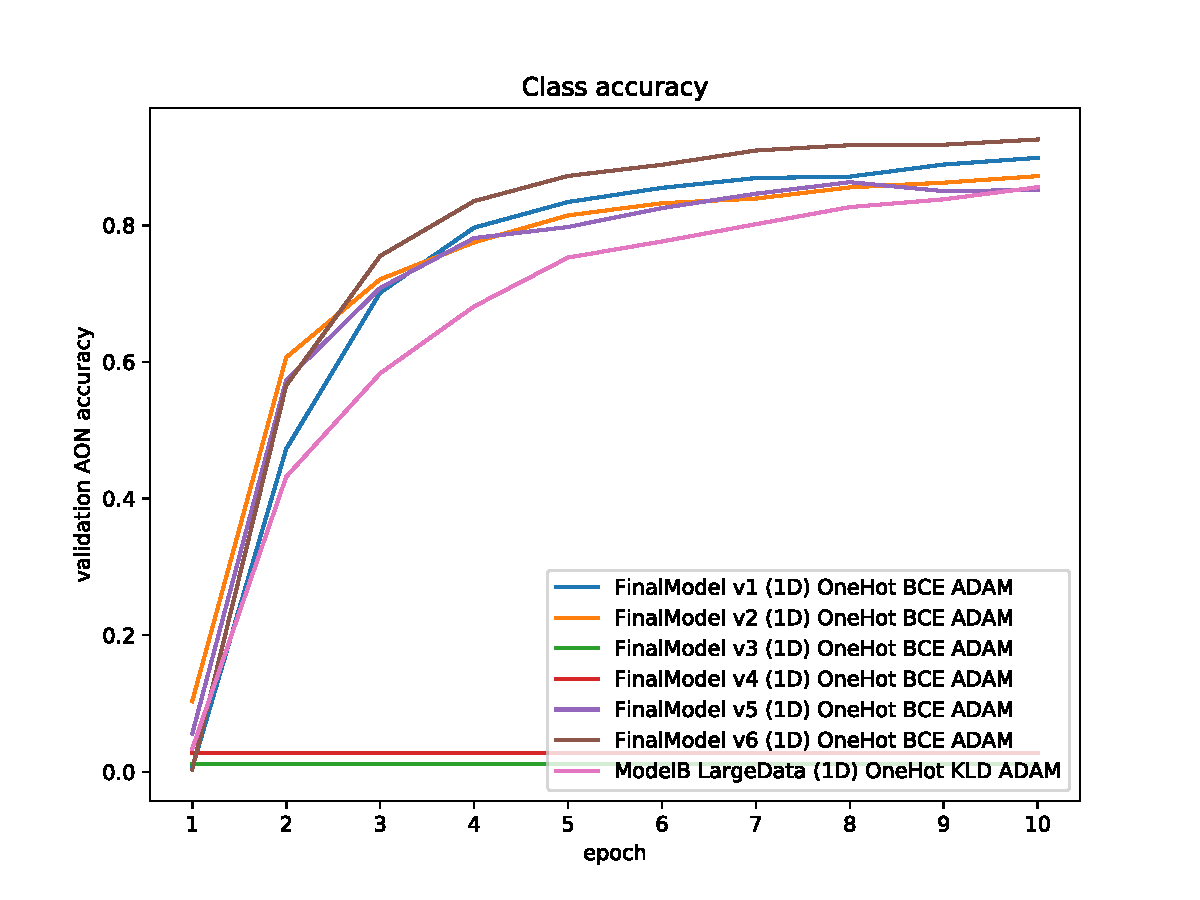
\includegraphics[width=0.75\textwidth]{figures/training_plots/FinalModelAccuracyComparison.pdf}
	    \caption{A comparison of the final models in class accuracy over 10 epochs.}
	    \label{fig:final_model_comparison}
	\end{figure}
	
	\subsection{Summary}
	
	Following the methodology, 3 out of the 4 objectives (see section \ref{sec:aim_and_obj}) were met: 3 neural network models were designed and tested using synthetic multi-classed data from processed, isolated hits; drum kit timbre was shown to be a trainable feature across all of the classes; and a model was trained to a high degree of accuracy with the synthetic data.\medskip
	
	The best performing model was Model B, the one-hot with KLD loss configuration reaching 83.8\% (AON) class accuracy when evaluated using the original testing data set. Using a larger batch size and a larger data set, Model B was re-trained and got to 85.8\% accuracy. Then, variations of Model B which tweaked depth, feature space and Leaky ReLU gradient were trained and tested, improving the accuracy to 92.4\%.\medskip
	
	This was close to the accuracy of the other drum kit classification model from the literature review (see section \ref{sec:previous_work}) which got 99\% accuracy, but this model classified 10 classes containing audio of similar timbres compared to the model in the literature, which classified 3 classes which had distinct timbres.\medskip
	
	Unfortunately, there was not enough time to apply this final model to real drum beats, which was the last objective. So it is not known how accurate these models are with real data.\medskip 
	
	\subsection{Future work}
    
    With more time, a 4\textsuperscript{th} model could have been made using 2D spectrogram data with a structure using inception modules; like in Model A. This was because only one model was made for 2D spectrogram data while 2 models were made for 1D amplitude data and this model design might have performed better than Model C, since the original NN which used the inception module design (GoogLeNet), was designed for 2D data \parencite{Oord2016}.\medskip
    
    In addition to varying the output encoding and the loss function, the width and depth of the models could have been varied to examine their effect on training and overall accuracy. However, these were kept constant until the final model so that there weren't too many factors; as these combinations of factors increases the amount of configurations per model and each model takes a lot of time to train per configuration.\medskip
    
    Since, there wasn't enough time to test this neural network model on real drum beats (it was only trained and tested on synthetic multi-classed hits), it isn't known how well it would perform on real data. This would be an interesting area to look into because even if the performance is slightly lower, the trained models can be adjusted to a higher accuracy, with less `real' data than is necessary for training models from scratch by using transfer learning \parencite{Asadi2007}.\medskip
    

	%Bibliography
	\newpage
	\nocite{*}
	\section{Bibliography}
	%Heading=subibnumbered with title adds a subsection to the tableofcontents
	%keyword restricts the sub reference of a specific   
	\medskip
	\printbibliography[notkeyword={figure}, title={References}]
	\printbibliography[type={misc}, keyword={figure}, title={Figures}]
	\newpage
	%Appendices
	\section{Appendices}
	% Appendices
\begin{appendices}
    \section{Input data}
        \subsection{Drum and cymbal classification}
        \label{app:classification}
        \texttt{Referred to in section \ref{sec:labelling_and_encoding}}\smallskip
        
        In \textit{settings.json} the type of hits, kit components and techniques used are described by the \textit{label} associative array. The combinations of these types which are valid classes are described by the  \textit{label-hierarchy} associative array. Here is the section of this file where they appear:
        
        \begin{lstlisting}
        "label": {
            "hit_label": ["beater", "stick"],
            "kit_label": [
              "bass_drum",
              "crash",
              "hi_hat",
              "high_tom",
              "mid_tom",
              "low_tom",
              "ride",
              "snare",
              "splash"
            ],
            "tech_label": ["bell", "normal", "open"]
        },
          
        "label-hierarchy": {
            "beater": { "bass_drum": ["normal"] },
            "stick": {
              "crash": ["normal"],
              "hi_hat": ["normal", "open"],
              "high_tom": ["normal"],
              "mid_tom": ["normal"],
              "low_tom": ["normal"],
              "ride": ["normal", "bell"],
              "snare": ["normal"]
            }
        }
        \end{lstlisting}
        
        Later the splash cymbal wasn't used because there wasn't enough raw data for it. Hence it doesn't appear in \textit{label-hierarchy} even though its still in \textit{label}.
        
        \newpage
        \subsection{Drum kit combinations}
        \label{app:kit-combinations}
        \texttt{Referred to in section \ref{sec:labelling_and_encoding}}\smallskip
        
        There are 87 different combinations of drum and cymbal that can be hit at once, since all drums and cymbals are hand operated apart from the bass drum and opening/closing hi-hat (not counting the hi-hat closing shut as a hit). The following list is how encodings were ordered:
        \begin{figure}[H]
            \centering
            \begin{tiny}
                \begin{tabular}{r|l|l|l|}
                    Index & \multicolumn{3}{c|}{Drum kit classes}\\
                    \hline
                    1 & bass-drum normal & & \\
                    \hline
                    2 & crash normal & & \\
                    \hline
                    3 & hi-hat normal & & \\
                    \hline
                    4 & hi-hat open & & \\
                    \hline
                    5 & high-tom normal & & \\
                    \hline
                    6 & low-tom normal & & \\
                    \hline
                    7 & mid-tom normal & & \\
                    \hline
                    8 & ride bell & & \\
                    \hline
                    9 & ride normal & & \\
                    \hline
                    10 & snare normal & & \\
                    \hline
                    11 & bass-drum normal & crash normal & \\
                    \hline
                    12 & bass-drum normal & hi-hat normal & \\
                    \hline
                    13 & bass-drum normal & hi-hat open & \\
                    \hline
                    14 & bass-drum normal & high-tom normal & \\
                    \hline
                    15 & bass-drum normal & low-tom normal & \\
                    \hline
                    16 & bass-drum normal & mid-tom normal & \\
                    \hline
                    17 & bass-drum normal & ride bell & \\
                    \hline
                    18 & bass-drum normal & ride normal & \\
                    \hline
                    19 & bass-drum normal & snare normal & \\
                    \hline
                    20 & crash normal & hi-hat normal & \\
                    \hline
                    21 & crash normal & hi-hat open & \\
                    \hline
                    22 & crash normal & high-tom normal & \\
                    \hline
                    23 & crash normal & low-tom normal & \\
                    \hline
                    24 & crash normal & mid-tom normal & \\
                    \hline
                    25 & crash normal & ride bell & \\
                    \hline
                    26 & crash normal & ride normal & \\
                    \hline
                    27 & crash normal & snare normal & \\
                    \hline
                    28 & hi-hat normal & high-tom normal & \\
                    \hline
                    29 & hi-hat normal & low-tom normal & \\
                    \hline
                    30 & hi-hat normal & mid-tom normal & \\
                    \hline
                    31 & hi-hat normal & ride bell & \\
                    \hline
                    32 & hi-hat normal & ride normal & \\
                    \hline
                    33 & hi-hat normal & snare normal & \\
                    \hline
                    34 & hi-hat open & high-tom normal & \\
                    \hline
                    35 & hi-hat open & low-tom normal & \\
                    \hline
                    36 & hi-hat open & mid-tom normal & \\
                    \hline
                    37 & hi-hat open & ride bell & \\
                    \hline
                    38 & hi-hat open & ride normal & \\
                    \hline
                    39 & hi-hat open & snare normal & \\
                    \hline
                    40 & high-tom normal & low-tom normal & \\
                    \hline
                    41 & high-tom normal & mid-tom normal & \\
                    \hline
                    42 & high-tom normal & ride bell & \\
                    \hline
                    43 & high-tom normal & ride normal & \\
                    \hline
                    44 & high-tom normal & snare normal & \\
                    \hline
                \end{tabular}
                \qquad
                \begin{tabular}{r|l|l|l|}
                    Index & \multicolumn{3}{c|}{Drum kit classes}\\
                    \hline
                    45 & low-tom normal & mid-tom normal & \\
                    \hline
                    46 & low-tom normal & ride bell & \\
                    \hline
                    47 & low-tom normal & ride normal & \\
                    \hline
                    48 & low-tom normal & snare normal & \\
                    \hline
                    49 & mid-tom normal & ride bell & \\
                    \hline
                    50 & mid-tom normal & ride normal & \\
                    \hline
                    51 & mid-tom normal & snare normal & \\
                    \hline
                    52 & ride bell & snare normal & \\
                    \hline
                    53 & ride normal & snare normal & \\
                    \hline
                    54 & bass-drum normal & crash normal & hi-hat normal \\
                    \hline
                    55 & bass-drum normal & crash normal & hi-hat open \\
                    \hline
                    56 & bass-drum normal & crash normal & high-tom normal \\
                    \hline
                    57 & bass-drum normal & crash normal & low-tom normal \\
                    \hline
                    58 & bass-drum normal & crash normal & mid-tom normal \\
                    \hline
                    59 & bass-drum normal & crash normal & ride bell \\
                    \hline
                    60 & bass-drum normal & crash normal & ride normal \\
                    \hline
                    61 & bass-drum normal & crash normal & snare normal \\
                    \hline
                    62 & bass-drum normal & hi-hat normal & high-tom normal \\
                    \hline
                    63 & bass-drum normal & hi-hat normal & low-tom normal \\
                    \hline
                    64 & bass-drum normal & hi-hat normal & mid-tom normal \\
                    \hline
                    65 & bass-drum normal & hi-hat normal & ride bell \\
                    \hline
                    66 & bass-drum normal & hi-hat normal & ride normal \\
                    \hline
                    67 & bass-drum normal & hi-hat normal & snare normal \\
                    \hline
                    68 & bass-drum normal & hi-hat open & high-tom normal \\
                    \hline
                    69 & bass-drum normal & hi-hat open & low-tom normal \\
                    \hline
                    70 & bass-drum normal & hi-hat open & mid-tom normal \\
                    \hline
                    71 & bass-drum normal & hi-hat open & ride bell \\
                    \hline
                    72 & bass-drum normal & hi-hat open & ride normal \\
                    \hline
                    73 & bass-drum normal & hi-hat open & snare normal \\
                    \hline
                    74 & bass-drum normal & high-tom normal & low-tom normal \\
                    \hline
                    75 & bass-drum normal & high-tom normal & mid-tom normal \\
                    \hline
                    76 & bass-drum normal & high-tom normal & ride bell \\
                    \hline
                    77 & bass-drum normal & high-tom normal & ride normal \\
                    \hline
                    78 & bass-drum normal & high-tom normal & snare normal \\
                    \hline
                    79 & bass-drum normal & low-tom normal & mid-tom normal \\
                    \hline
                    80 & bass-drum normal & low-tom normal & ride bell \\
                    \hline
                    81 & bass-drum normal & low-tom normal & ride normal \\
                    \hline
                    82 & bass-drum normal & low-tom normal & snare normal \\
                    \hline
                    83 & bass-drum normal & mid-tom normal & ride bell \\
                    \hline
                    84 & bass-drum normal & mid-tom normal & ride normal \\
                    \hline
                    85 & bass-drum normal & mid-tom normal & snare normal \\
                    \hline
                    86 & bass-drum normal & ride bell & snare normal \\
                    \hline
                    87 & bass-drum normal & ride normal & snare normal \\
                    \hline
                \end{tabular}
            \end{tiny}
            \caption*{Valid drum kit combinations}
        \end{figure}
    
    \newpage
    \section{Model structure}
    \label{app:model_structure}
        \subsection{Model A}
        \label{app:modelA_diagram}
        \texttt{Referred to in section \ref{sec:design_modelA}}
        \begin{figure}[H]
            \centering
            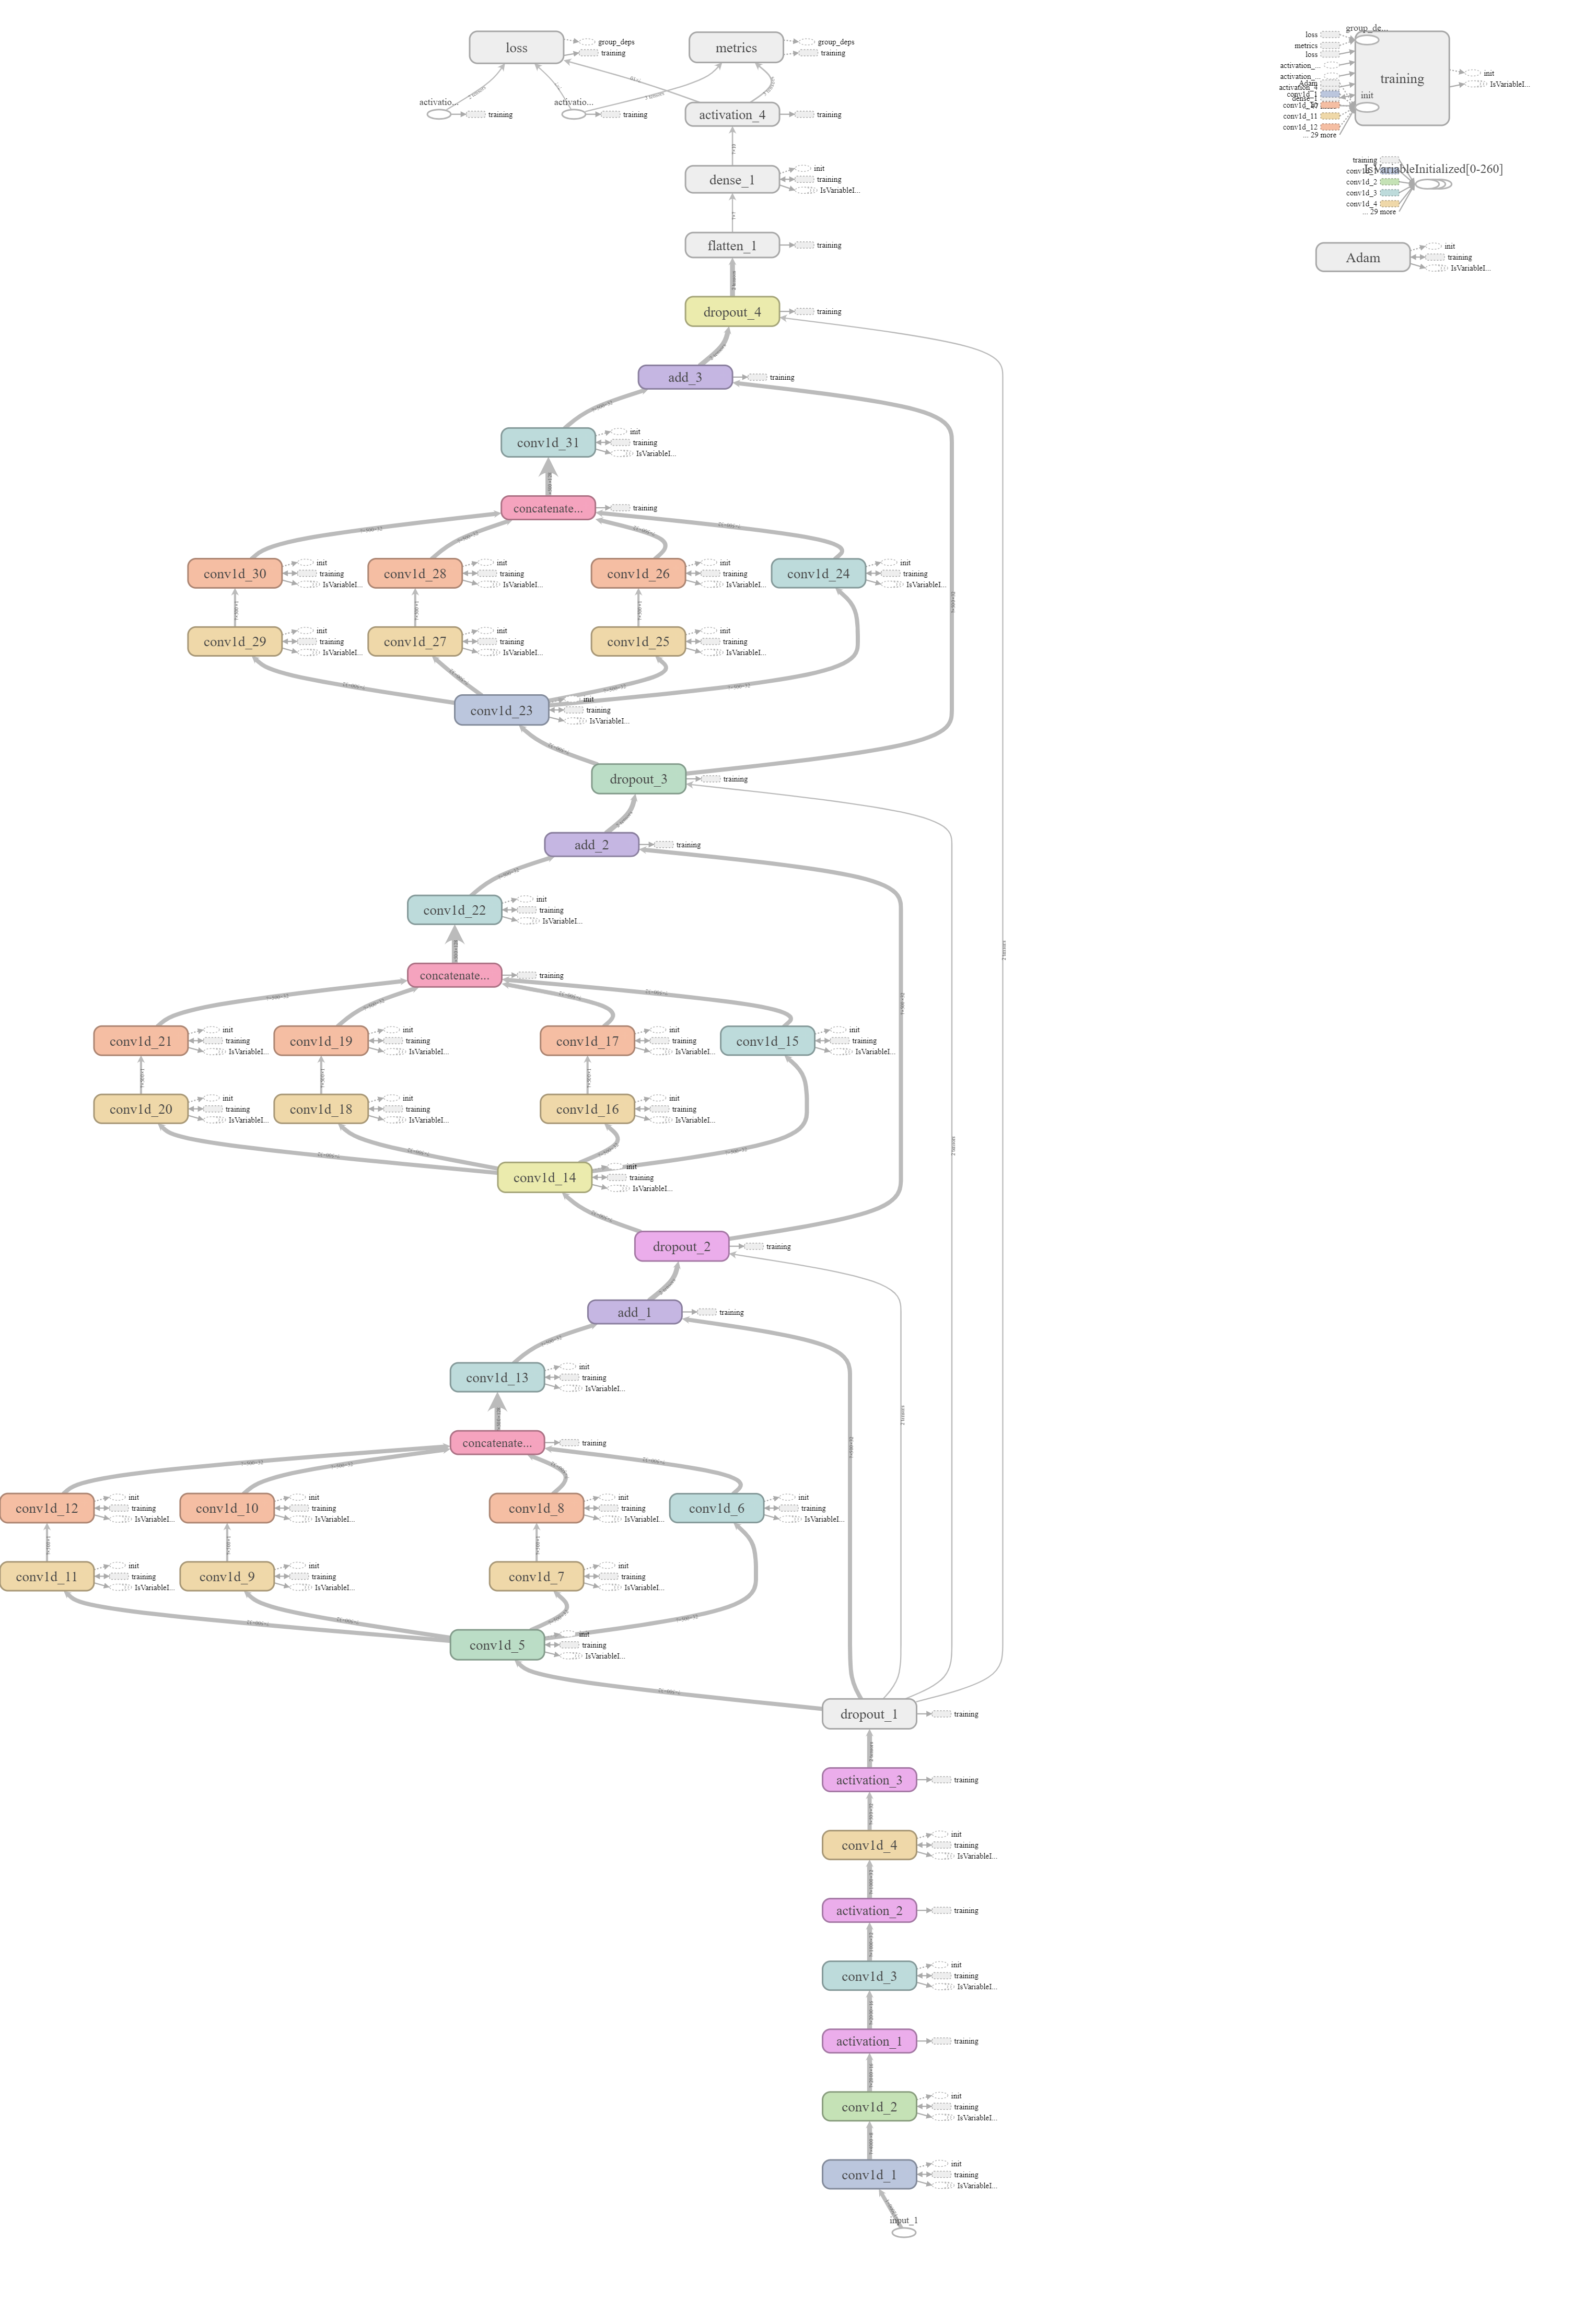
\includegraphics[height=0.85\textheight]{figures/modelA_diagram.png}
            \caption*{TensorBoard diagram of Model A.}
        \end{figure}
        
        \subsection{Model B}
        \label{app:modelB_diagram}
        \texttt{Referred to in section \ref{sec:design_modelB}}
        \begin{figure}[H]
            \centering
            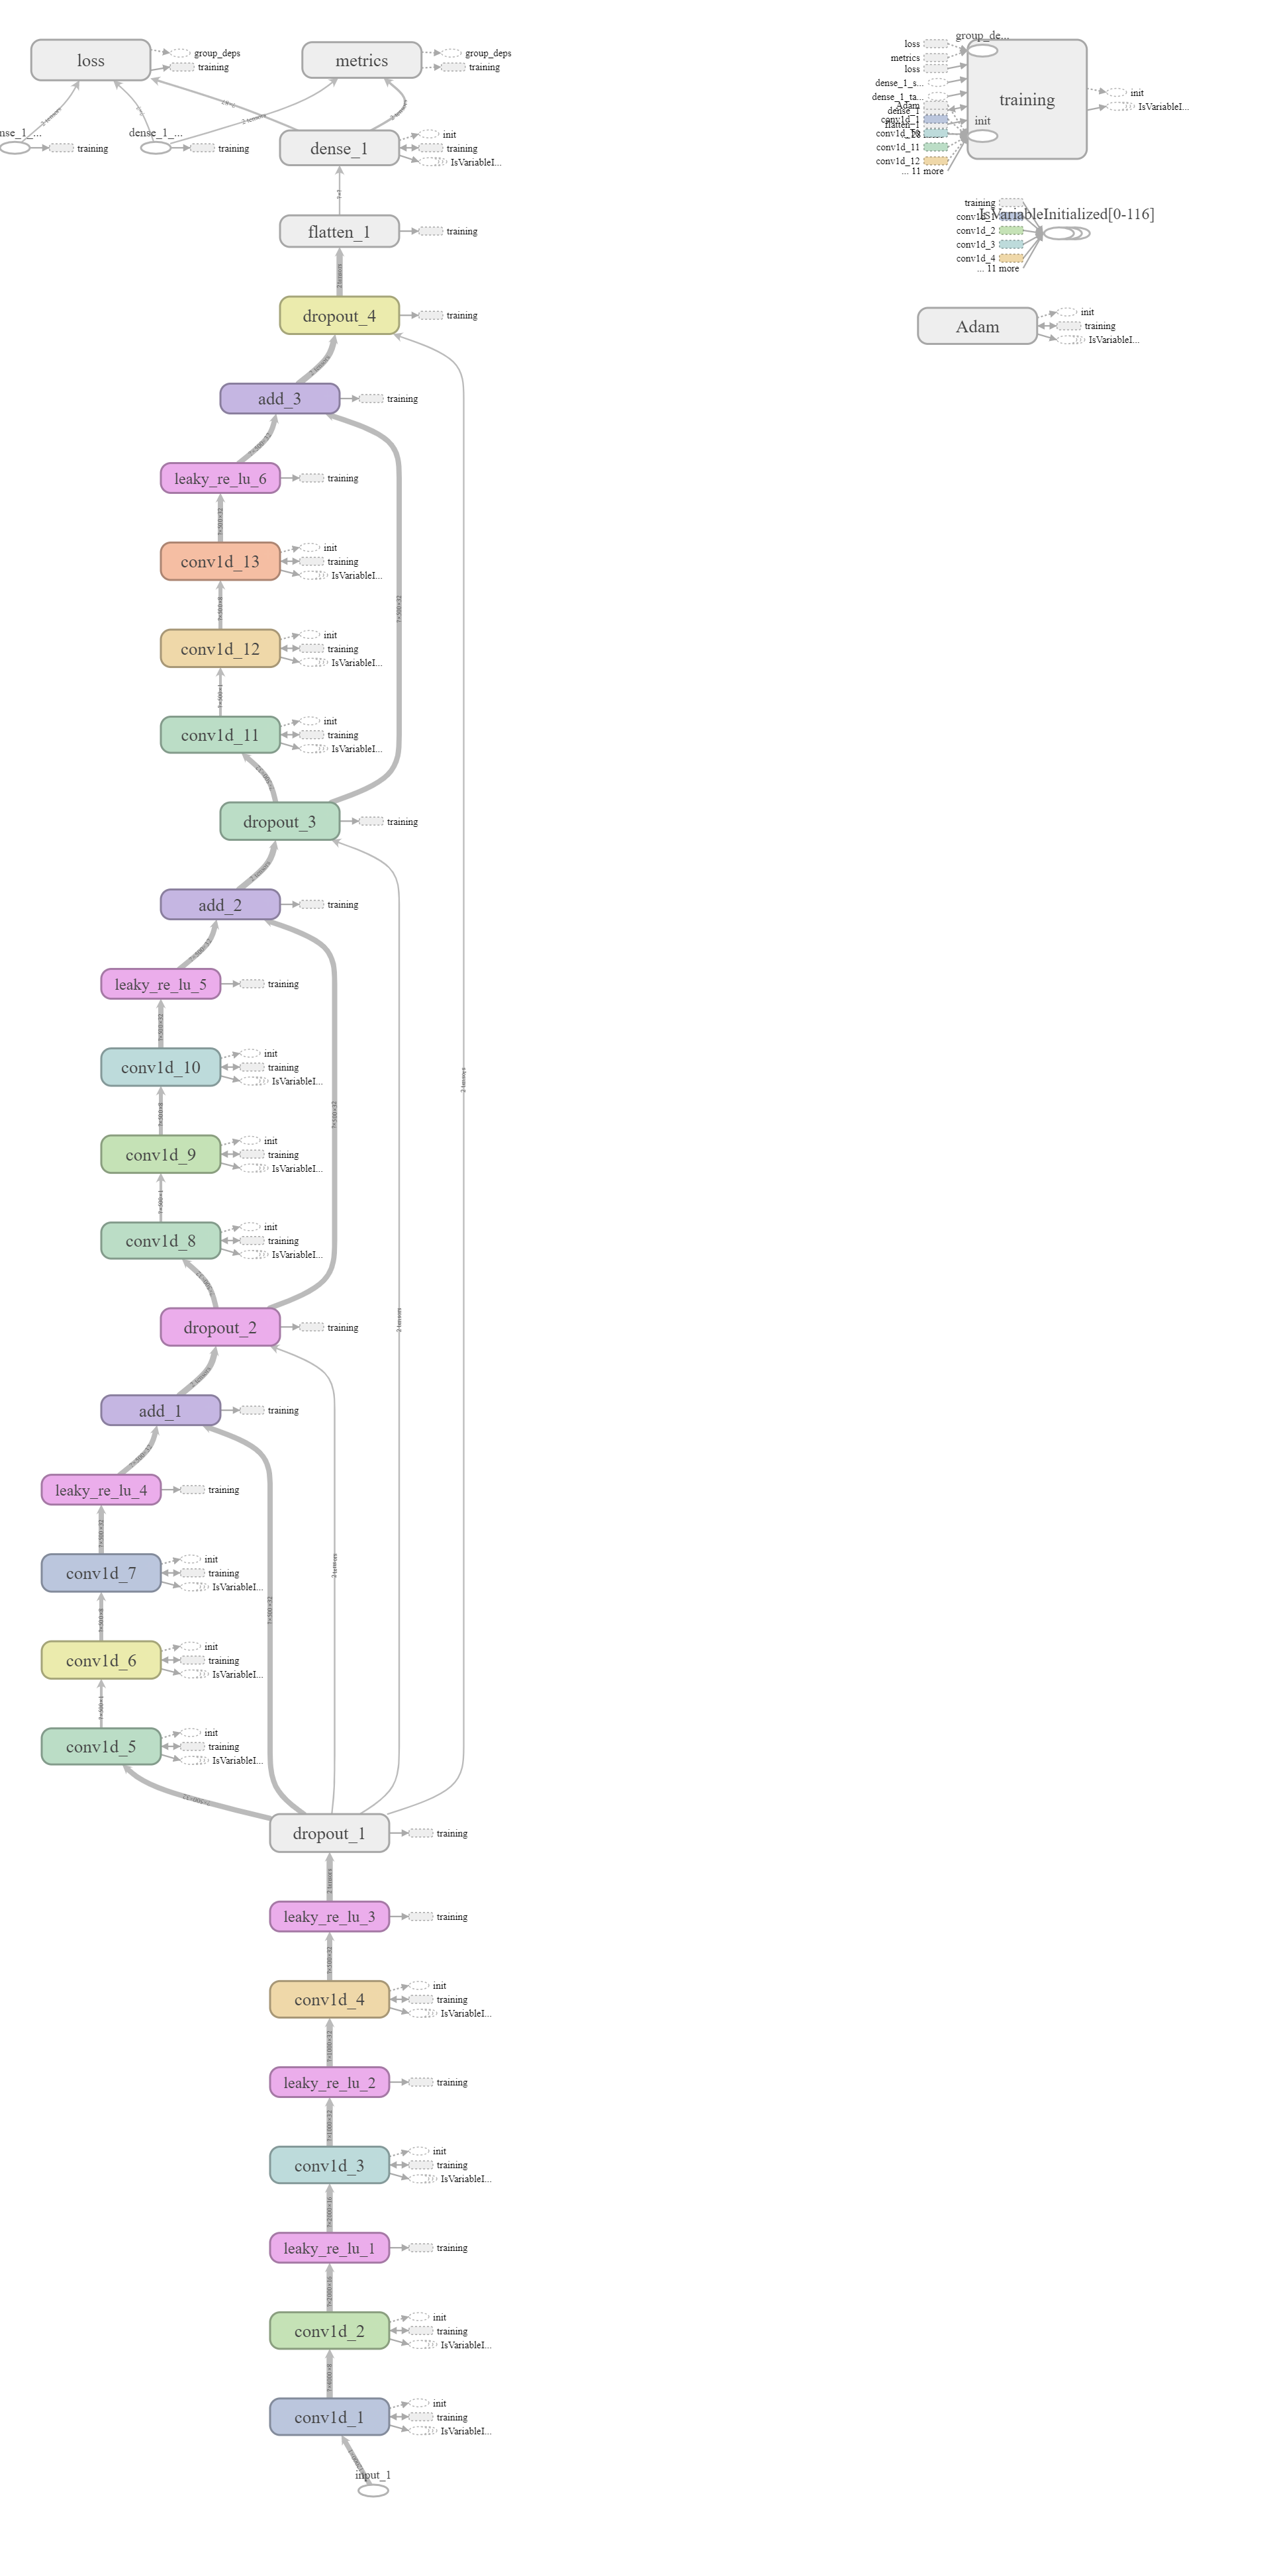
\includegraphics[height=0.85\textheight]{figures/modelB_diagram.png}
            \caption*{TensorBoard diagram of Model B.}
        \end{figure}
        
        \subsection{Model C}
        \label{app:modelC_diagram}
        \texttt{Referred to in section \ref{sec:design_modelC}}
        \begin{figure}[H]
            \centering
            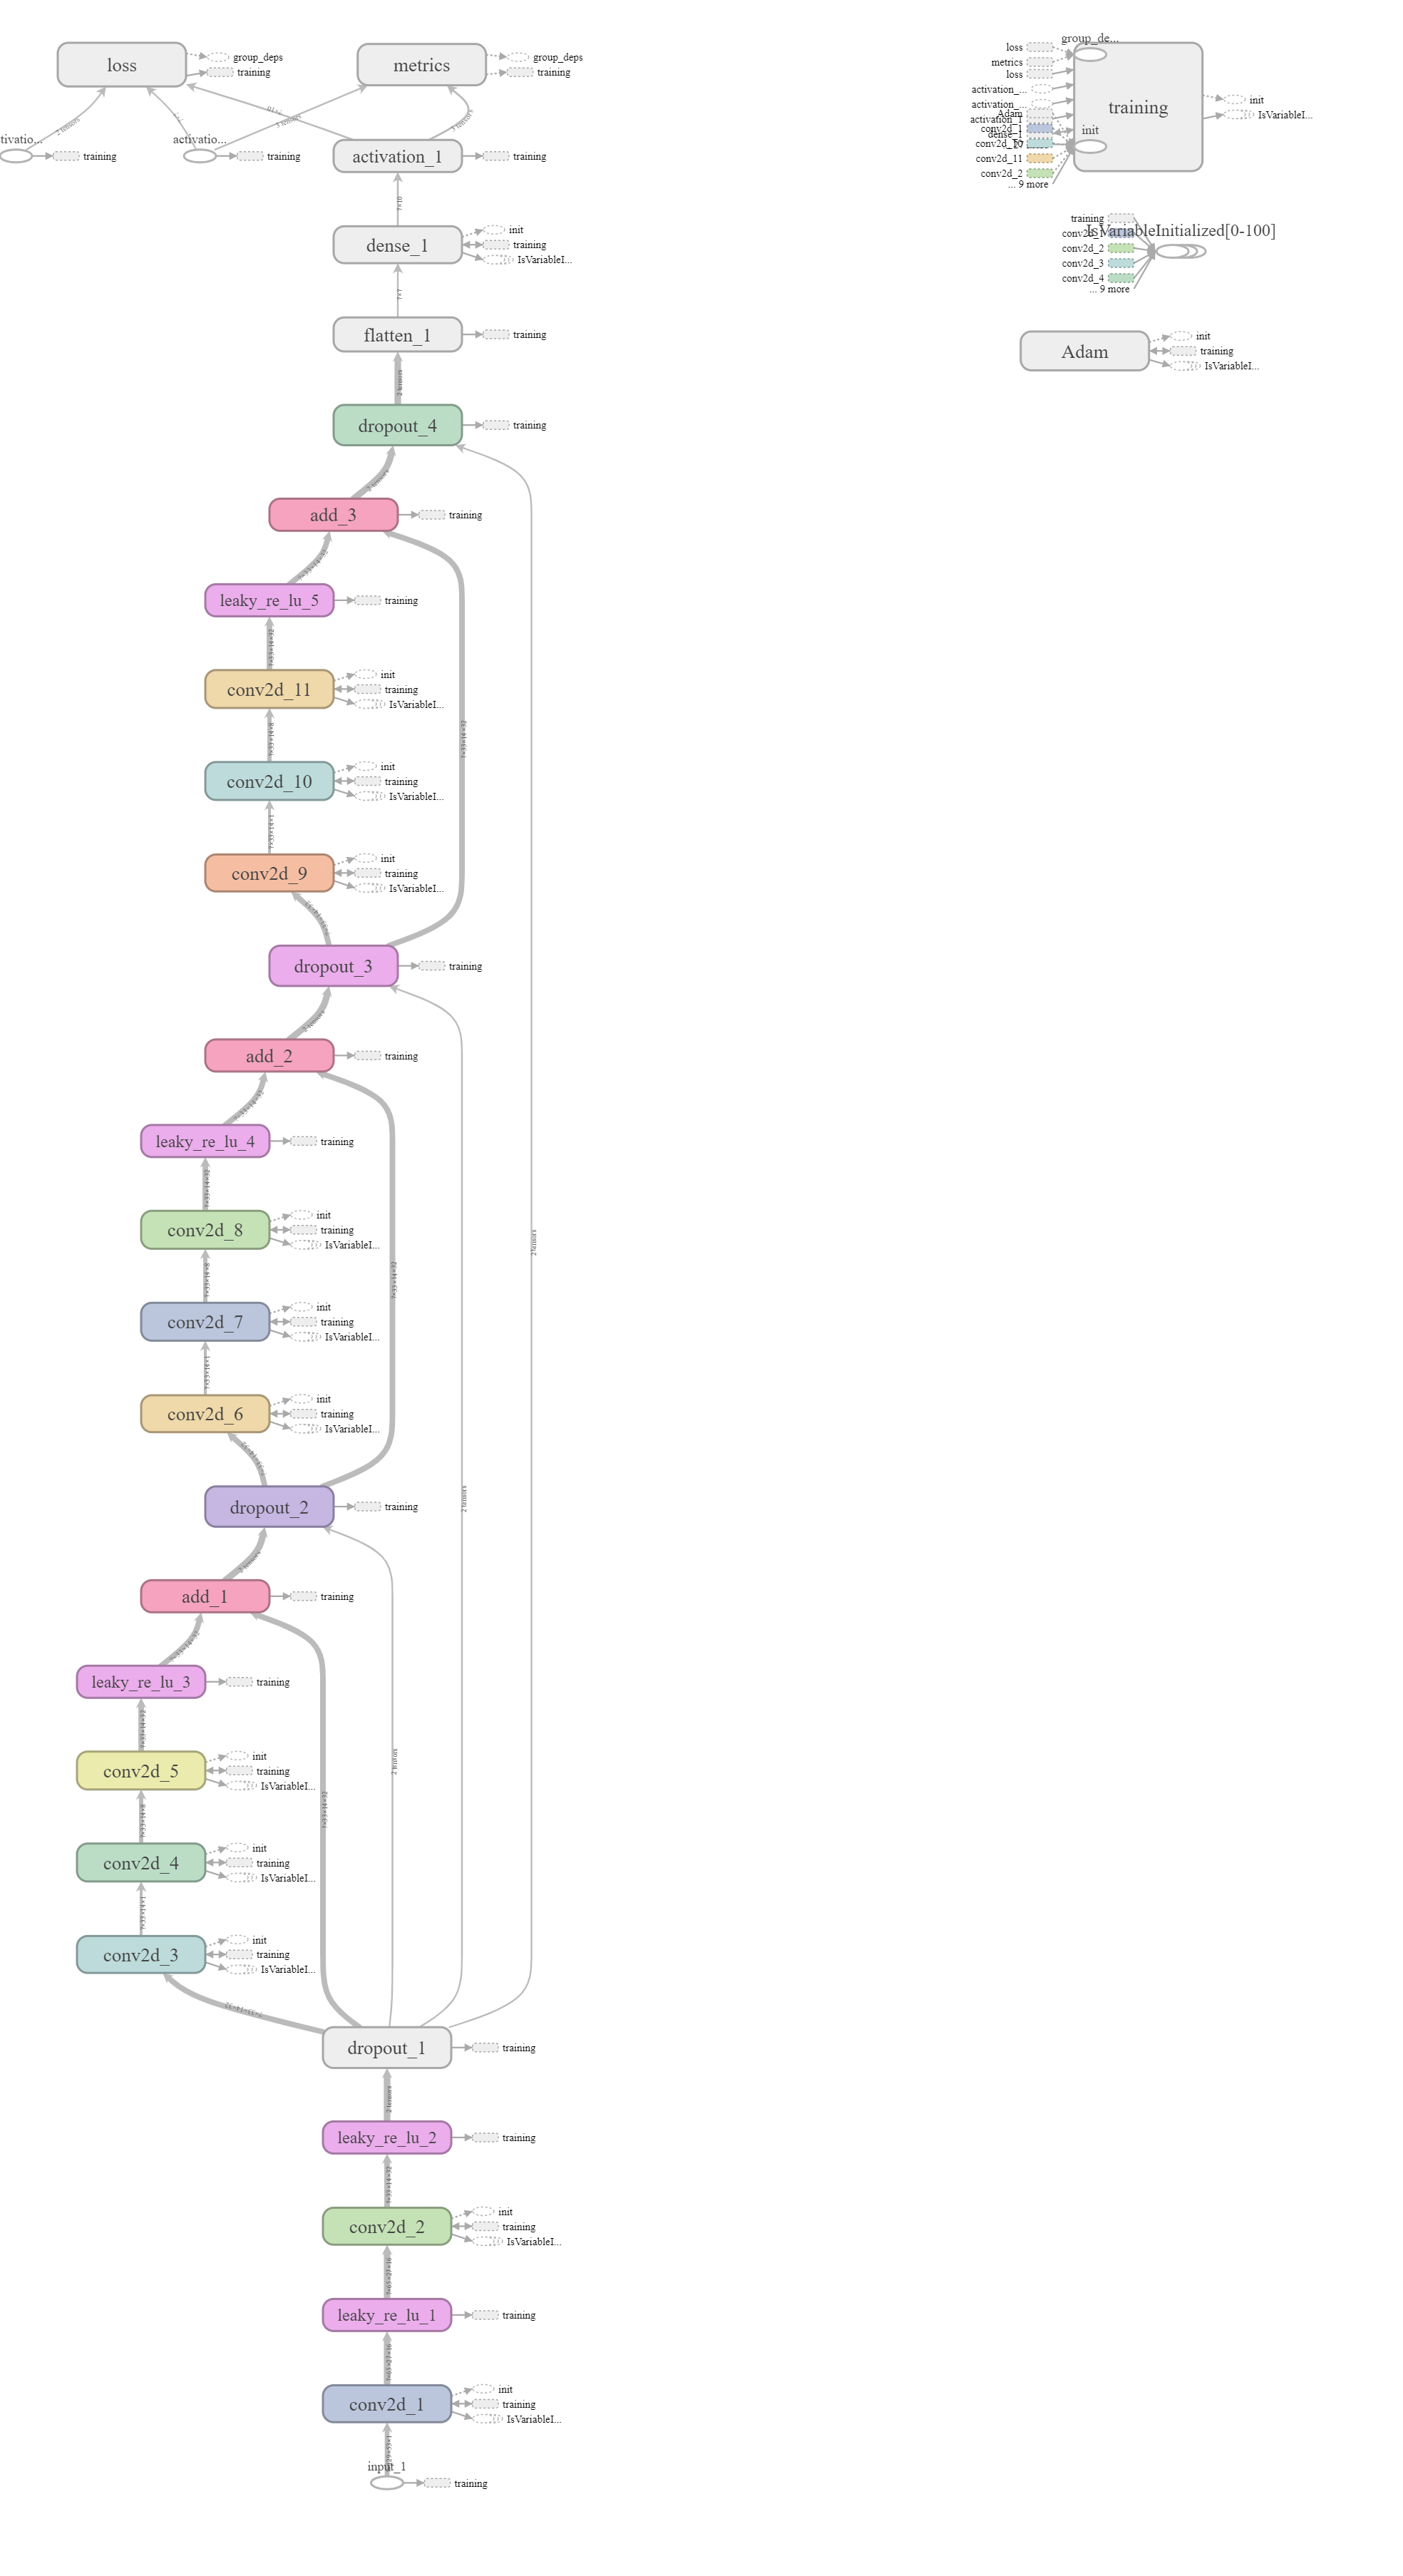
\includegraphics[height=0.85\textheight]{figures/modelC_diagram.png}
            \caption*{TensorBoard diagram of Model C.}
        \end{figure}
    
    \newpage
    \section{Training progress}
        \subsection{Optimisation algorithm comparison}
        \subsubsection{Loss during training}
        \label{app:optimisation_loss_during_training}
        \texttt{Referred to in section \ref{sec:training_analysis}}
        
        \begin{figure}[H]
            \centering
            \begin{tabular}{l|c|}
                Optimiser & Loss and validation loss during training\\
                \hline
                SGD & 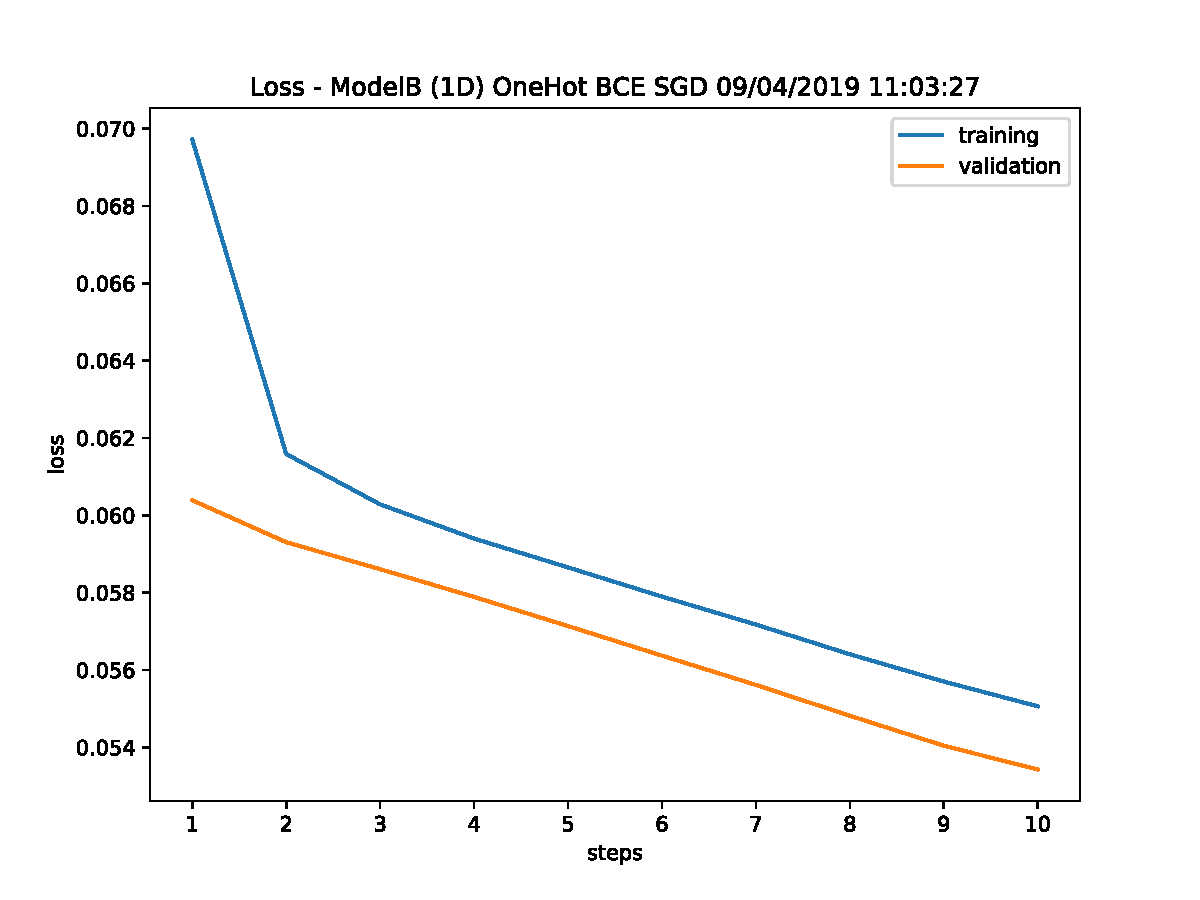
\includegraphics[width=0.7\textwidth,height=0.22\textheight,keepaspectratio]{figures/training_plots/ModelB-(1D)-OneHot-BCE-SGD_09-04-2019_11-03-27_loss.pdf}\\
                \hline
                ADAGRAD & 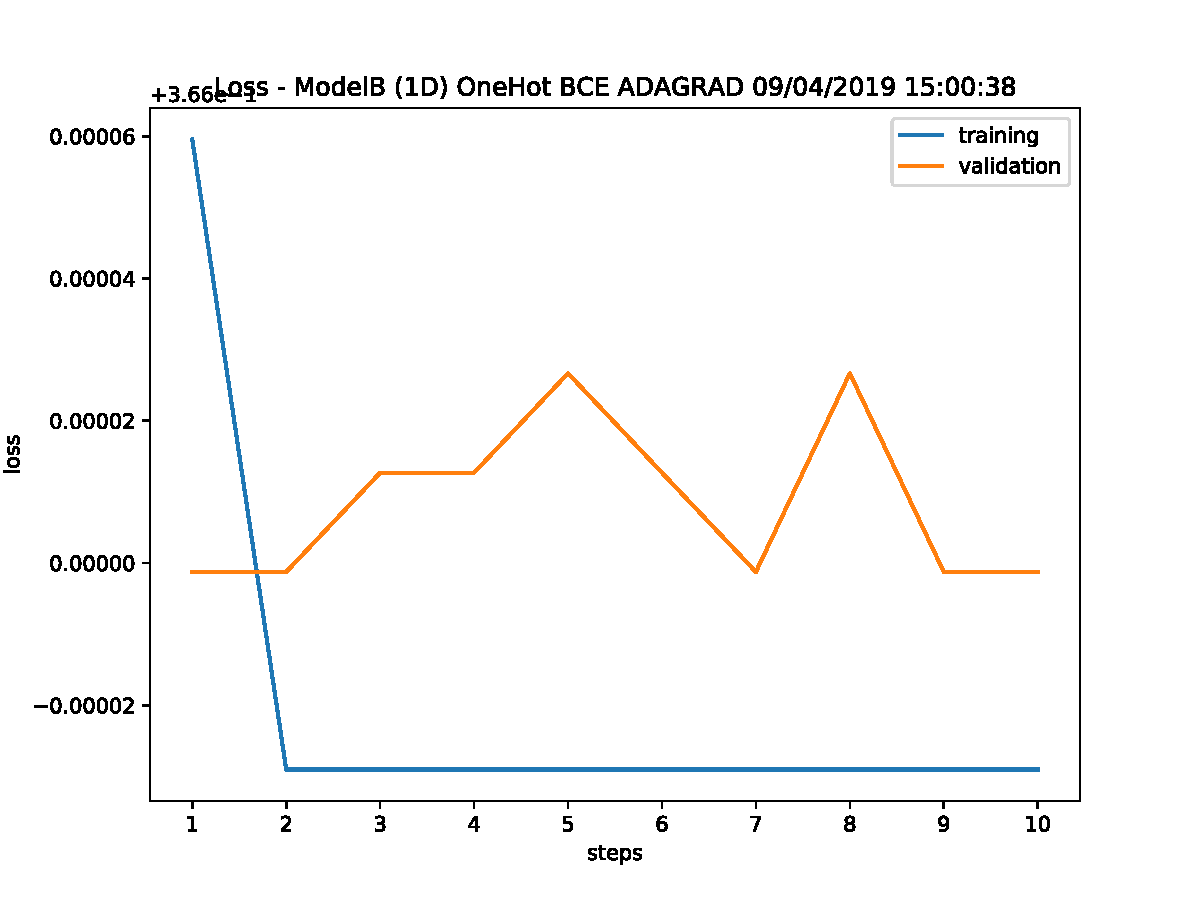
\includegraphics[width=0.7\textwidth,height=0.22\textheight,keepaspectratio]{figures/training_plots/ModelB-(1D)-OneHot-BCE-ADAGRAD_09-04-2019_15-00-38_loss.pdf}\\
                \hline
                ADAM & 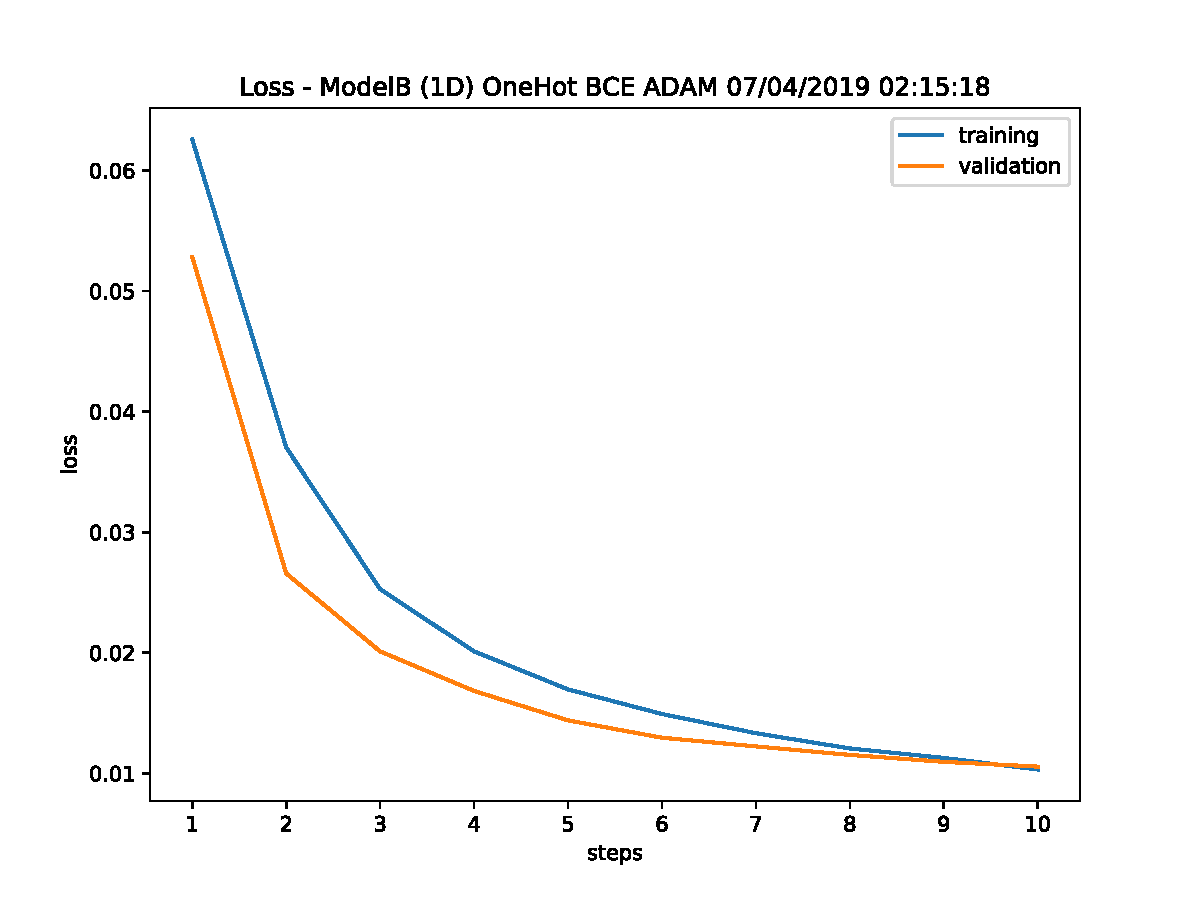
\includegraphics[width=0.7\textwidth,height=0.22\textheight,keepaspectratio]{figures/training_plots/ModelB-(1D)-OneHot-BCE-ADAM_07-04-2019_02-15-18_loss.pdf} 
            \end{tabular}
            \caption*{The loss values during training for Model B with one-hot encoding and BCE loss when using different optimiser algorithms. \textit{Note: the vertical scale of the middle figure (for ADAGRAD) is +0.366.}}
        \end{figure}
        
        \subsubsection{Training processing times}
        \label{app:optimisation_processing_times}
        \texttt{Referred to in section \ref{sec:training_analysis}}
        
        \begin{figure}[H]
            \centering
            \begin{tabular}{l|c|c|c|c|c|c|c|c|c|c|c|}
                \multirow{2}{*}{Optimiser} & \multicolumn{10}{c|}{Epoch} & \multirow{2}{*}{Total}\\
                    \cline{2-11}
                    & 1 & 2 & 3 & 4 & 5 & 6 & 7 & 8 & 9 & 10 &\\
                    \hline
                ADAGRAD & 24.0 & 23.0 & 23.1 & 25.1 & 21.4 & 24.3 & 26.9 & 22.3 & 22.2 & 24.8 & 237.0\\
                ADAM & 24.3 & 19.0 & 19.0 & 19.0 & 19.1 & 19.0 & 18.9 & 19.1 & 19.0 & 18.9 & 195.3\\
                SGD & 23.6 & 22.3 & 22.7 & 28.4 & 21.8 & 24.2 & 19.3 & 18.9 & 19.0 & 18.9 & 219.0
            \end{tabular}
            \caption*{The duration of each epoch as well as total time taken for 10 epochs in minutes. For different optimisation algorithms on Model B with one-hot encoding and BCE loss.}
        \end{figure}
        
        \subsection{All model processing times with ADAM optimiser}
        \label{app:model_processing_times}
        \texttt{Referred to in section \ref{sec:training_analysis}}
        
        \begin{figure}[H]
            \centering
            \begin{footnotesize}
                \begin{tabular}{l|c|c|c|c|c|c|c|c|c|c|c|}
                    \multirow{2}{*}{Model and configuration} & \multicolumn{10}{c|}{Epoch} & \multirow{2}{*}{Total}\\
                    \cline{2-11}
                    & 1 & 2 & 3 & 4 & 5 & 6 & 7 & 8 & 9 & 10 &\\
                    \hline
                    ModelA (1D) MultiHot BCE & 24.8 & 19.6 & 19.1 & 19.3 & 19.2 & 19.2 & 19.3 & 19.4 & 19.1 & 19.2 & 198.1\\
                    ModelA (1D) MultiHot KLD & 25.7 & 20.2 & 19.5 & 19.4 & 19.3 & 21.8 & 22.7 & 25.9 & 19.2 & 19.2 & 212.8\\
                    ModelA (1D) OneHot BCE & 35.6 & 44.4 & 42.7 & 46.6 & 43.1 & 43.3 & 42.2 & 42.5 & 42.2 & 43.5 & 426.0\\
                    ModelA (1D) OneHot KLD & 24.0 & 24.5 & 26.5 & 34.6 & 20.2 & 19.4 & 19.5 & 19.3 & 19.5 & 19.5 & 227.0\\
                    ModelB (1D) MultiHot BCE & 24.3 & 27.3 & 22.2 & 19.0 & 18.7 & 18.7 & 19.0 & 19.1 & 18.8 & 18.9 & 205.9\\
                    ModelB (1D) MultiHot KLD & 25.8 & 22.6 & 20.2 & 20.7 & 20.2 & 20.2 & 20.4 & 20.2 & 20.1 & 20.2 & 210.6\\
                    ModelB (1D) OneHot BCE & 24.3 & 19.0 & 19.0 & 19.0 & 19.1 & 19.0 & 18.9 & 19.1 & 19.0 & 18.9 & 195.3\\
                    ModelB (1D) OneHot KLD & 24.7 & 19.2 & 18.8 & 19.0 & 19.0 & 18.9 & 19.0 & 19.1 & 19.3 & 19.3 & 196.4\\
                    ModelC (lin 2D) MultiHot BCE & 24.3 & 18.8 & 19.0 & 19.0 & 19.0 & 19.1 & 19.0 & 19.0 & 19.3 & 23.9 & 200.3\\
                    ModelC (lin 2D) MultiHot KLD & 24.8 & 24.1 & 29.4 & 32.5 & 22.7 & 19.2 & 19.1 & 19.0 & 19.0 & 19.2 & 229.0\\
                    ModelC (lin 2D) OneHot BCE & 24.2 & 19.0 & 19.0 & 19.0 & 19.0 & 18.9 & 18.9 & 19.3 & 19.0 & 18.9 & 195.1\\
                    ModelC (lin 2D) OneHot KLD & 23.4 & 18.8 & 19.0 & 19.1 & 23.6 & 24.7 & 24.9 & 25.5 & 22.6 & 25.4 & 227.0\\
                    ModelC (log 2D) MultiHot BCE & 24.6 & 19.0 & 19.1 & 19.3 & 19.2 & 18.9 & 19.0 & 19.1 & 19.0 & 19.0 & 196.2\\
                    ModelC (log 2D) MultiHot KLD & 24.3 & 18.9 & 18.9 & 31.3 & 21.4 & 19.0 & 26.8 & 19.5 & 19.2 & 19.2 & 218.4\\
                    ModelC (log 2D) OneHot BCE & 23.0 & 23.3 & 25.6 & 23.9 & 19.4 & 20.0 & 19.5 & 20.0 & 19.3 & 20.2 & 214.2\\
                    ModelC (log 2D) OneHot KLD & 24.5 & 26.4 & 28.2 & 33.8 & 22.8 & 27.8 & 30.0 & 20.7 & 38.0 & 26.7 & 278.7
                \end{tabular}
            \end{footnotesize}
            \caption*{The duration of each epoch as well as total time taken for 10 epochs in minutes. For different models using ADAM optimisation.}
        \end{figure}
        
        \newpage
        \subsection{Model A training metrics}
        \label{app:modelA_training}
        \texttt{Referred to in section \ref{sec:training_analysis_modelA}}
        
        \begin{figure}[H]
            \centering
            \begin{tabular}{cc}
                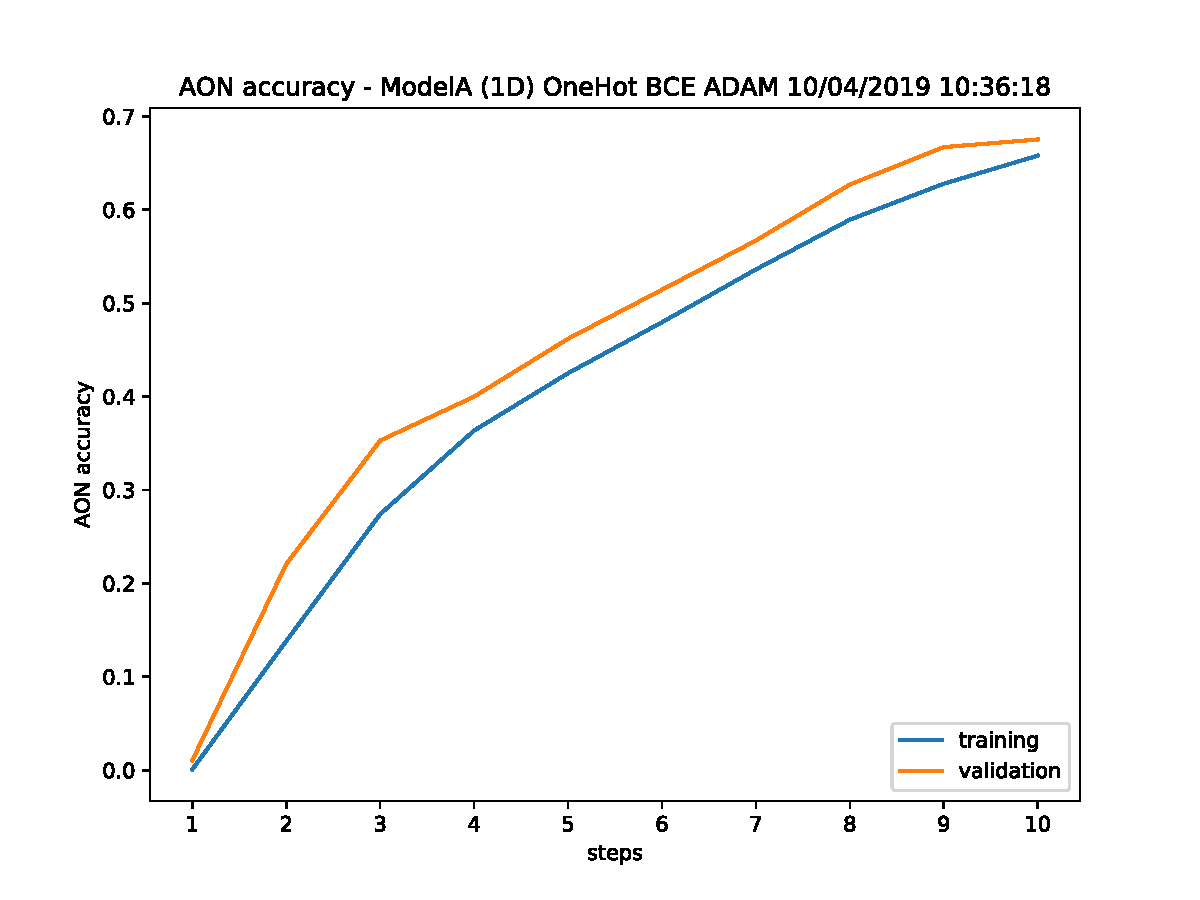
\includegraphics[width=0.45\textwidth]{figures/training_plots/ModelA-(1D)-OneHot-BCE-ADAM_10-04-2019_10-36-18_AON-accuracy.pdf} & 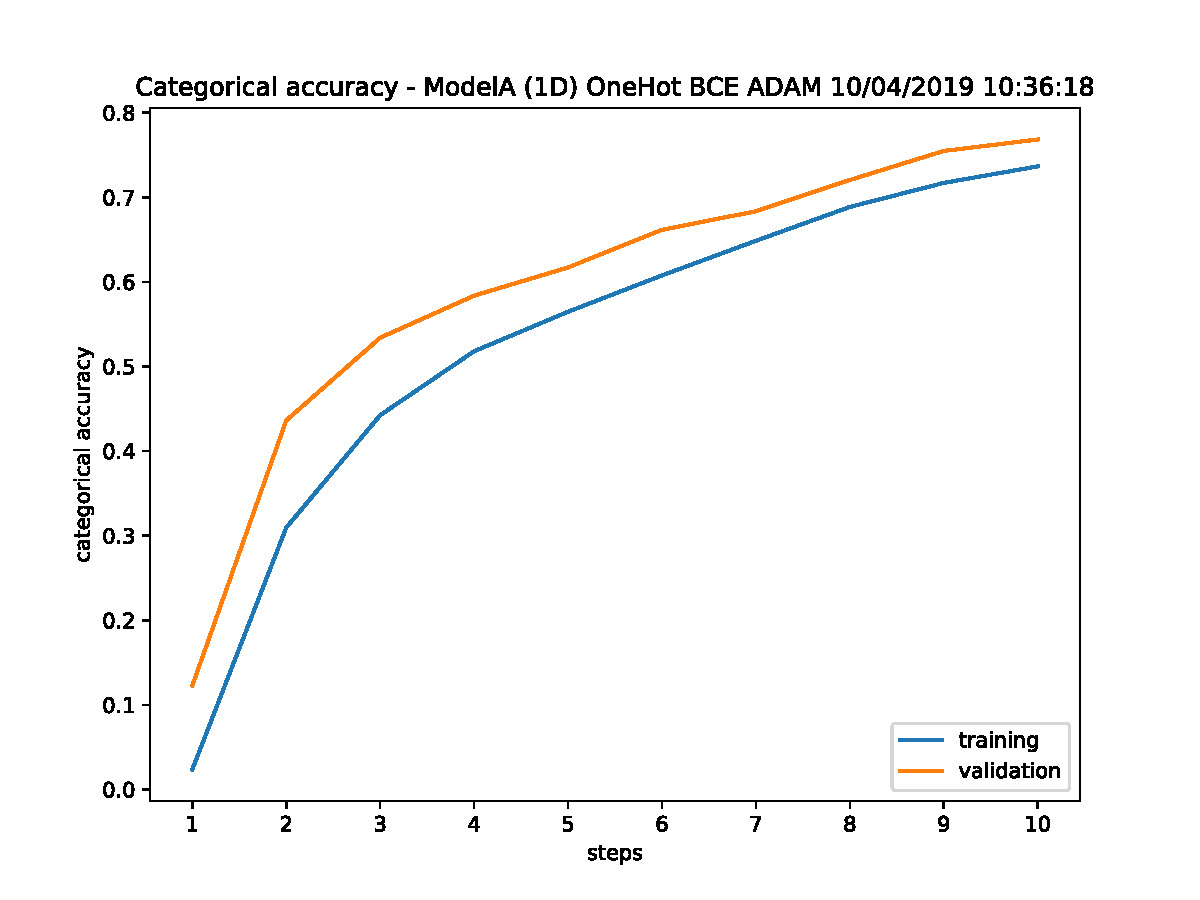
\includegraphics[width=0.45\textwidth]{figures/training_plots/ModelA-(1D)-OneHot-BCE-ADAM_10-04-2019_10-36-18_categorical-accuracy.pdf} \\
                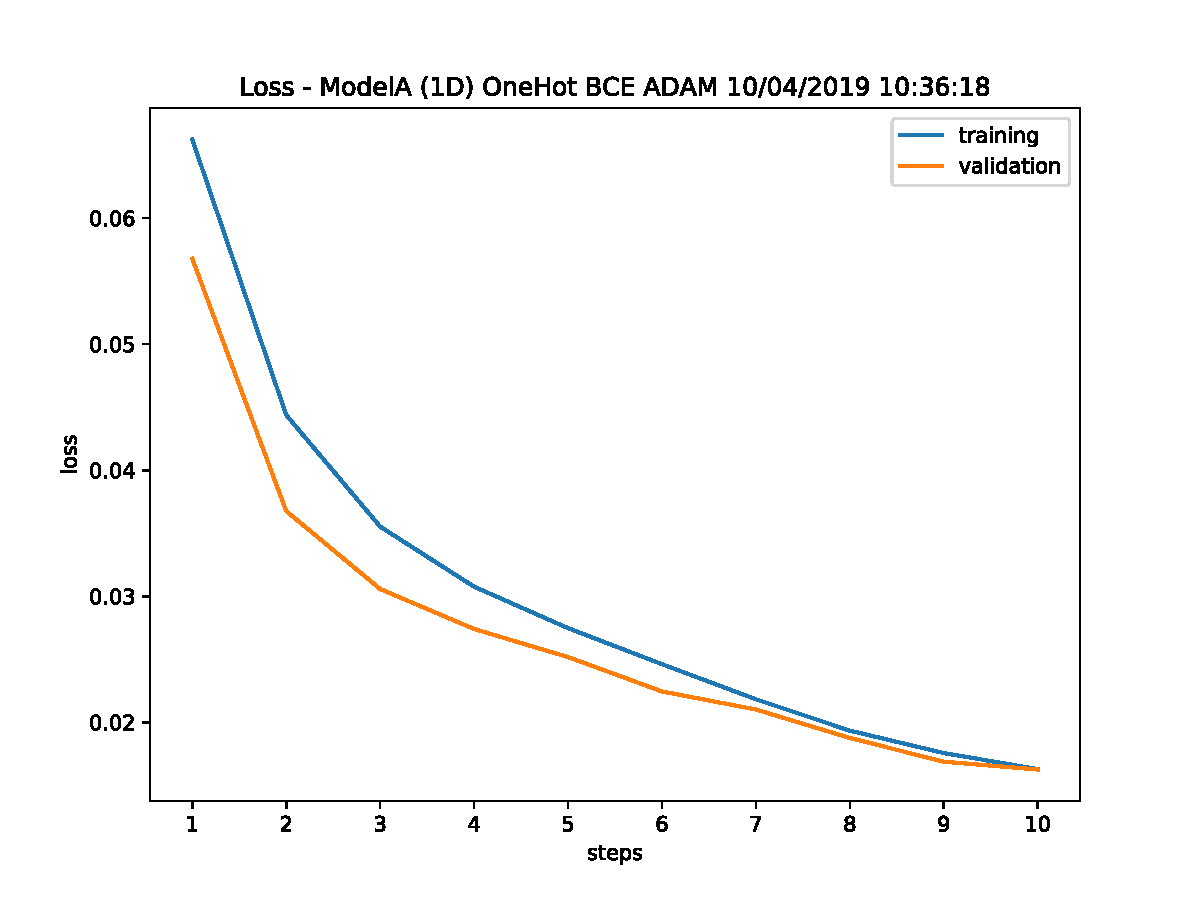
\includegraphics[width=0.45\textwidth]{figures/training_plots/ModelA-(1D)-OneHot-BCE-ADAM_10-04-2019_10-36-18_loss.pdf} & 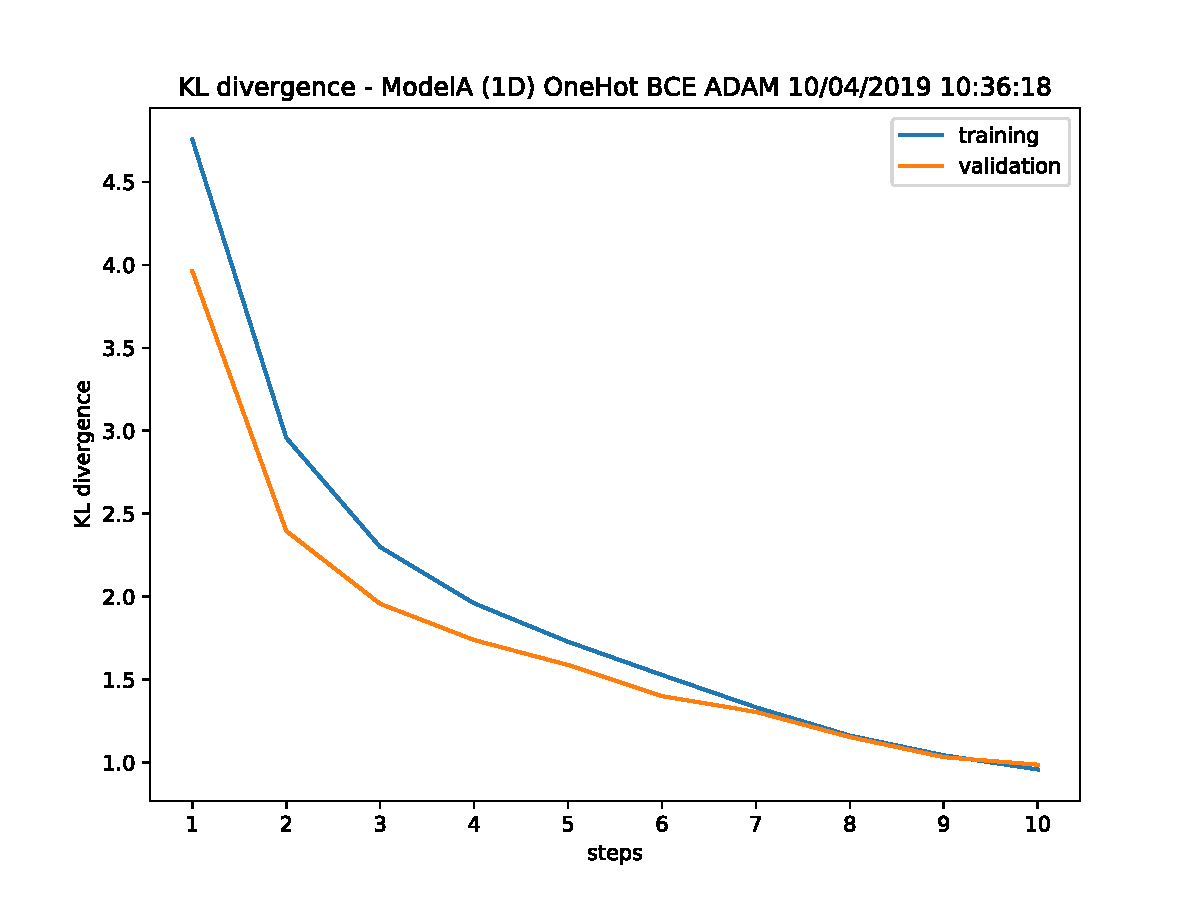
\includegraphics[width=0.45\textwidth]{figures/training_plots/ModelA-(1D)-OneHot-BCE-ADAM_10-04-2019_10-36-18_KL-divergence.pdf}
            \end{tabular}
            \caption*{One-hot encoding, BCE loss}
        \end{figure}
        
        \begin{figure}[H]
            \centering
            \begin{tabular}{cc}
                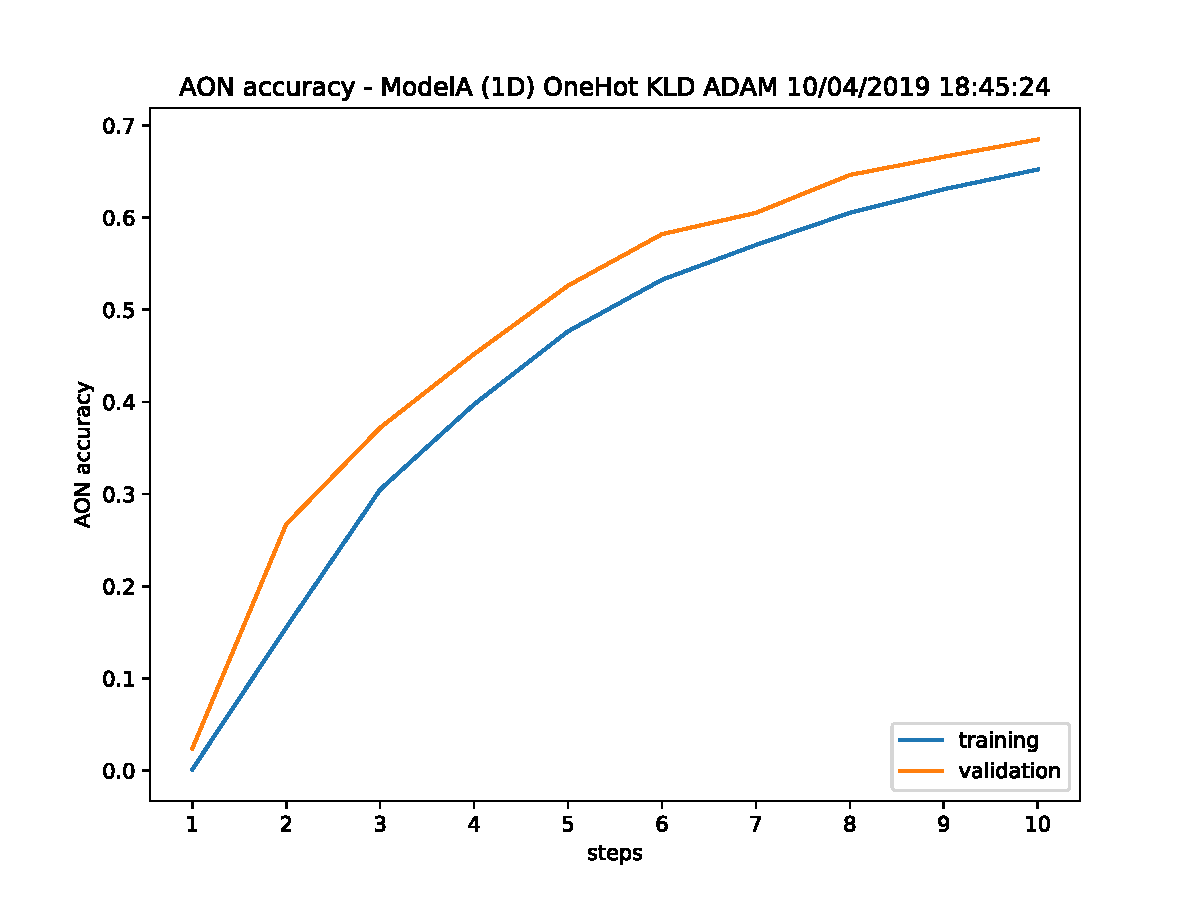
\includegraphics[width=0.45\textwidth]{figures/training_plots/ModelA-(1D)-OneHot-KLD-ADAM_10-04-2019_18-45-24_AON-accuracy.pdf} & 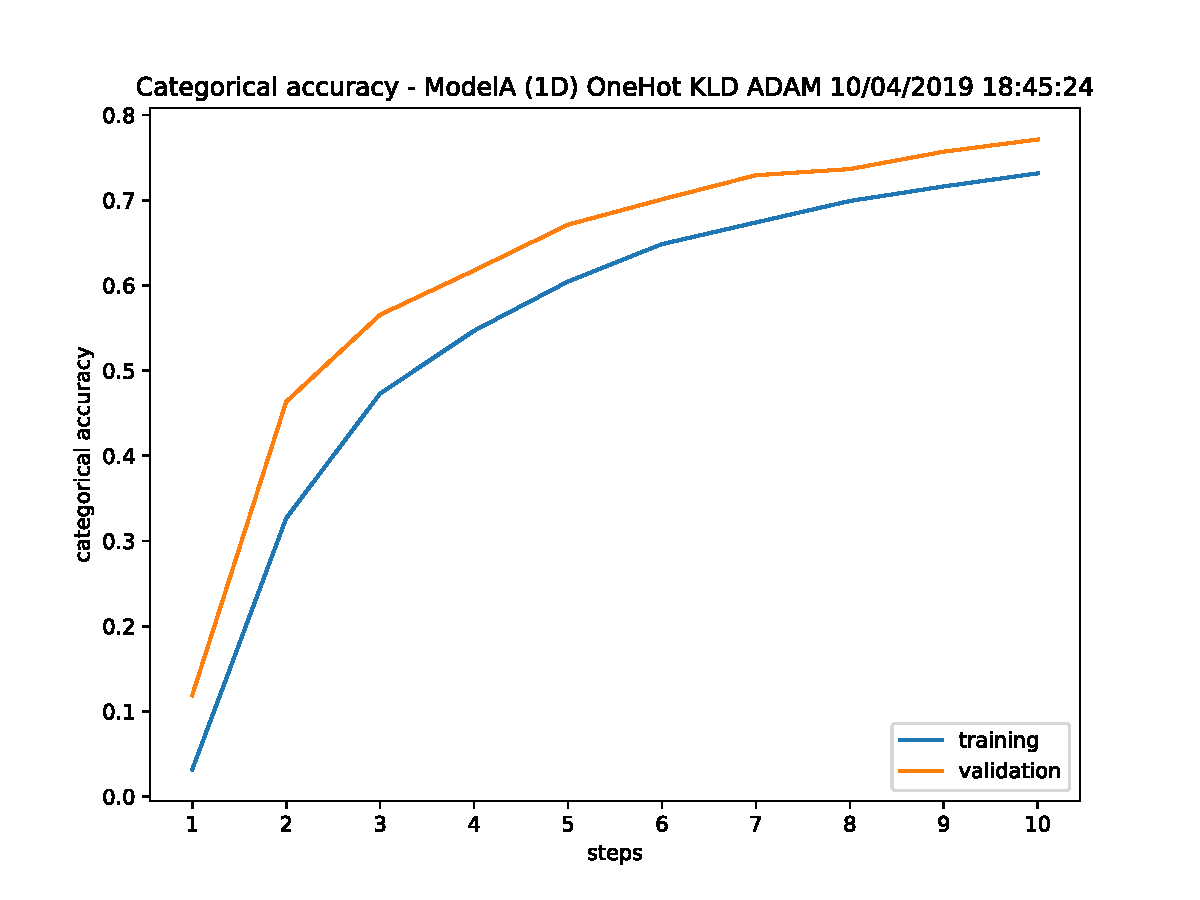
\includegraphics[width=0.45\textwidth]{figures/training_plots/ModelA-(1D)-OneHot-KLD-ADAM_10-04-2019_18-45-24_categorical-accuracy.pdf} \\
                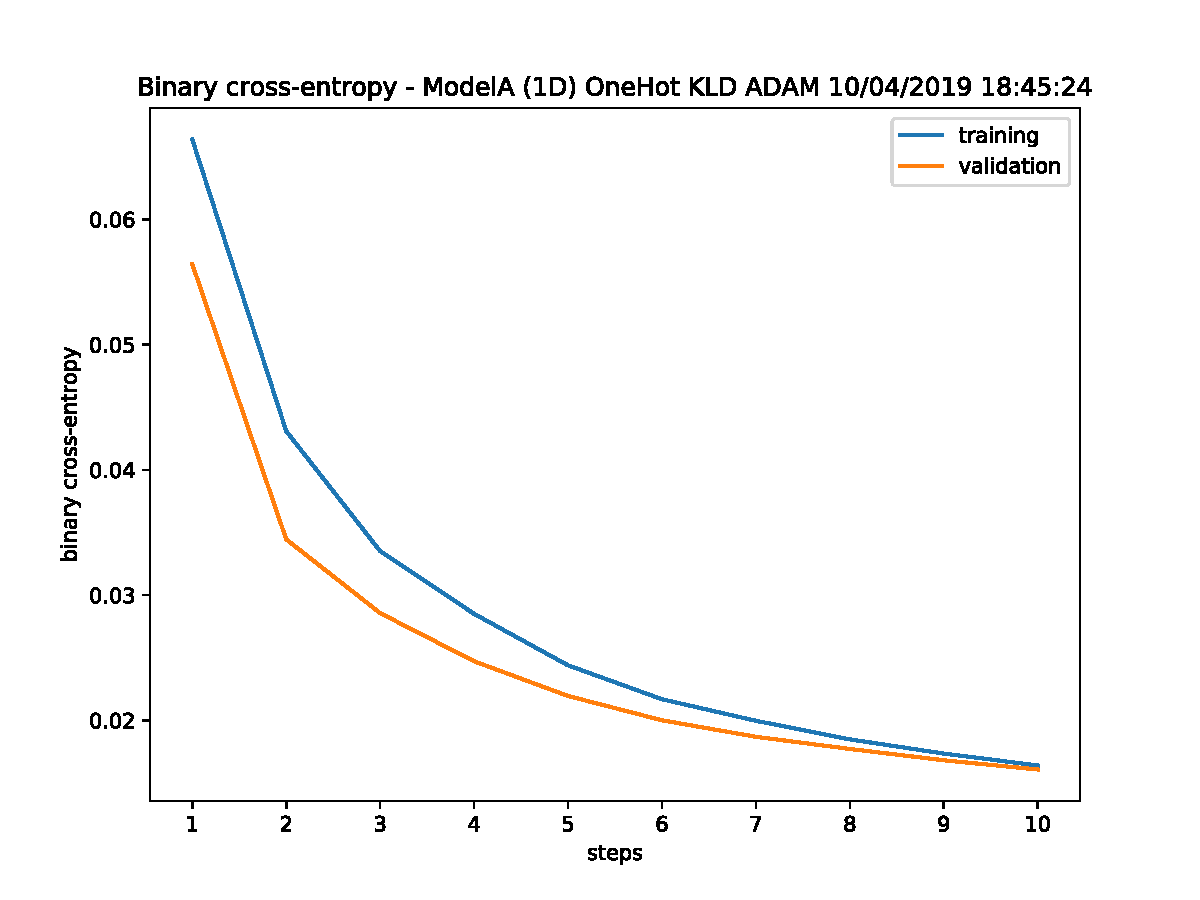
\includegraphics[width=0.45\textwidth]{figures/training_plots/ModelA-(1D)-OneHot-KLD-ADAM_10-04-2019_18-45-24_binary-cross-entropy.pdf} & 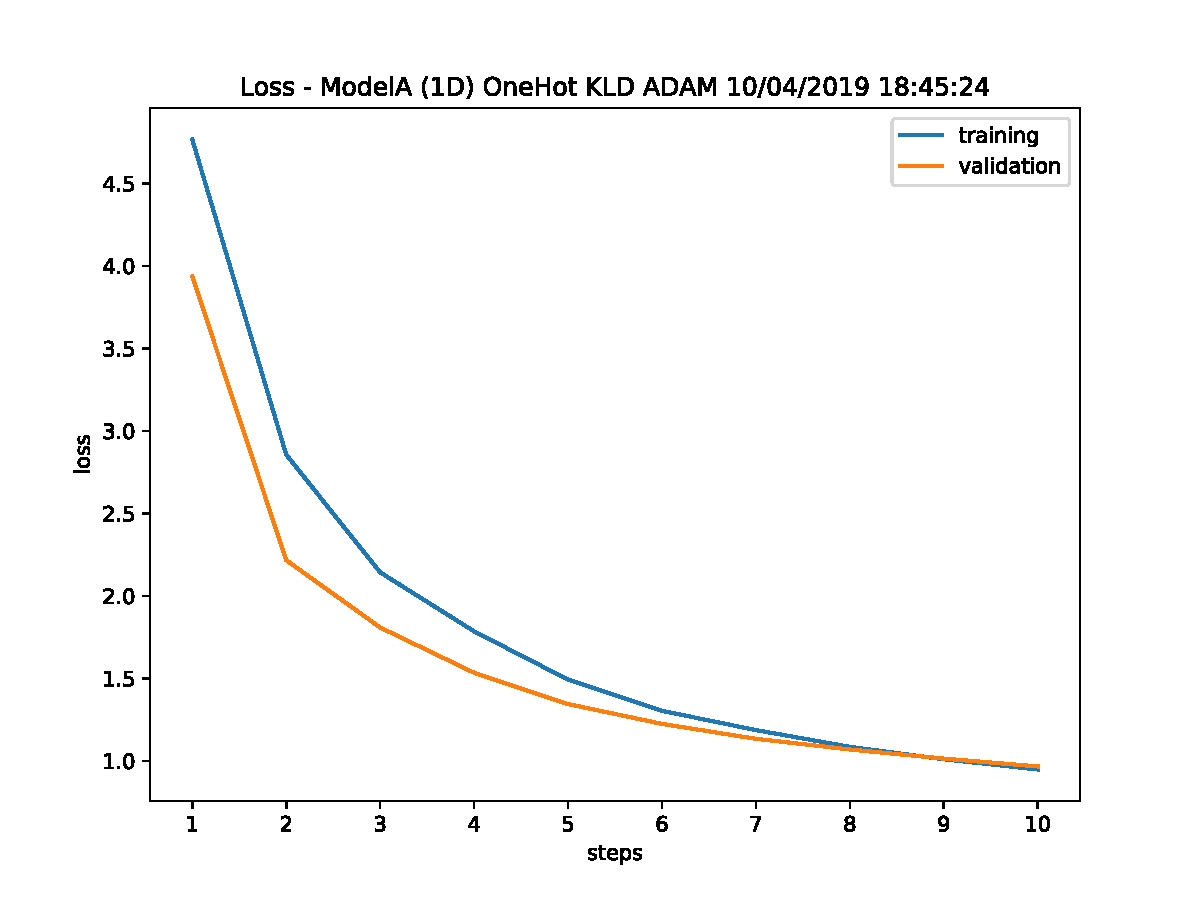
\includegraphics[width=0.45\textwidth]{figures/training_plots/ModelA-(1D)-OneHot-KLD-ADAM_10-04-2019_18-45-24_loss.pdf}
            \end{tabular}
            \caption*{One-hot encoding, KLD loss}
        \end{figure}
        
        \begin{figure}[H]
            \centering
            \begin{tabular}{cc}
                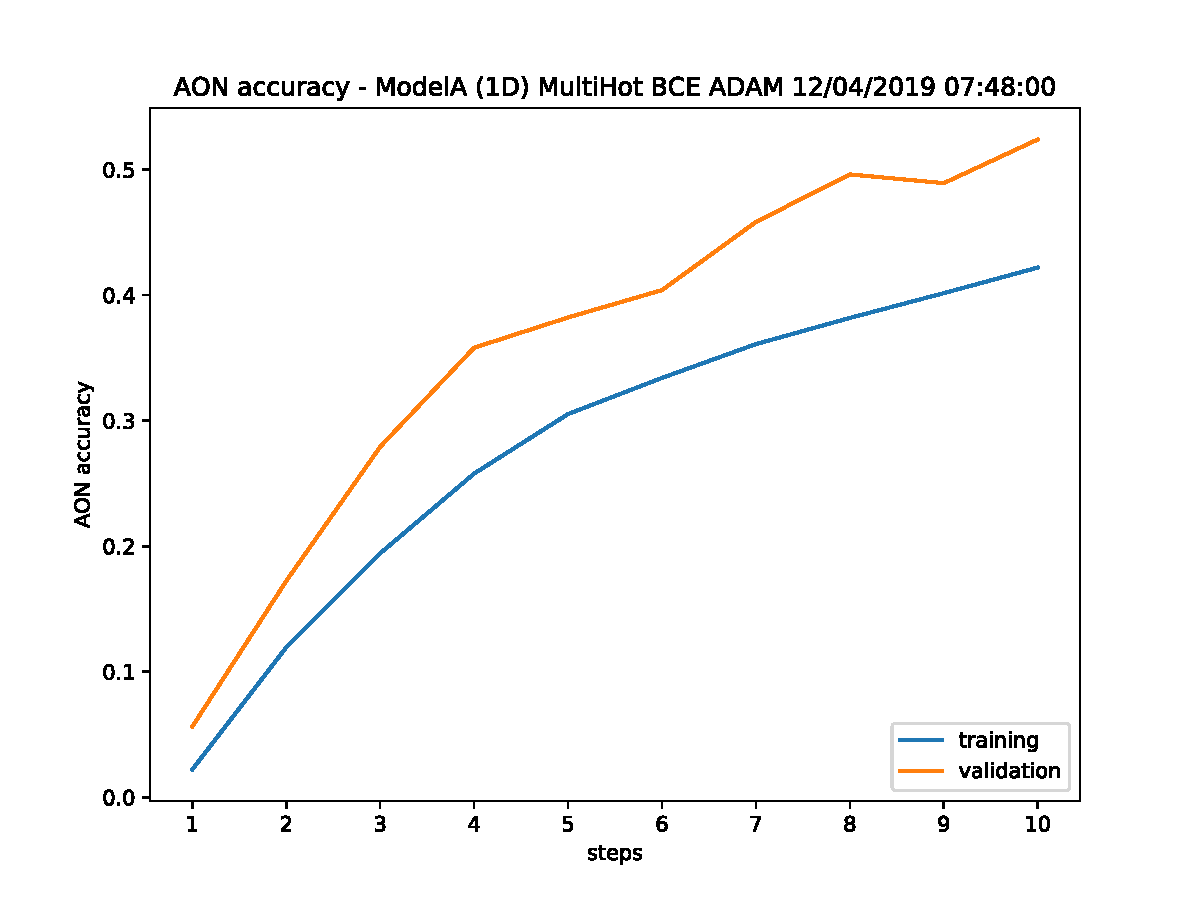
\includegraphics[width=0.48\textwidth]{figures/training_plots/ModelA-(1D)-MultiHot-BCE-ADAM_12-04-2019_07-48-00_AON-accuracy.pdf} & 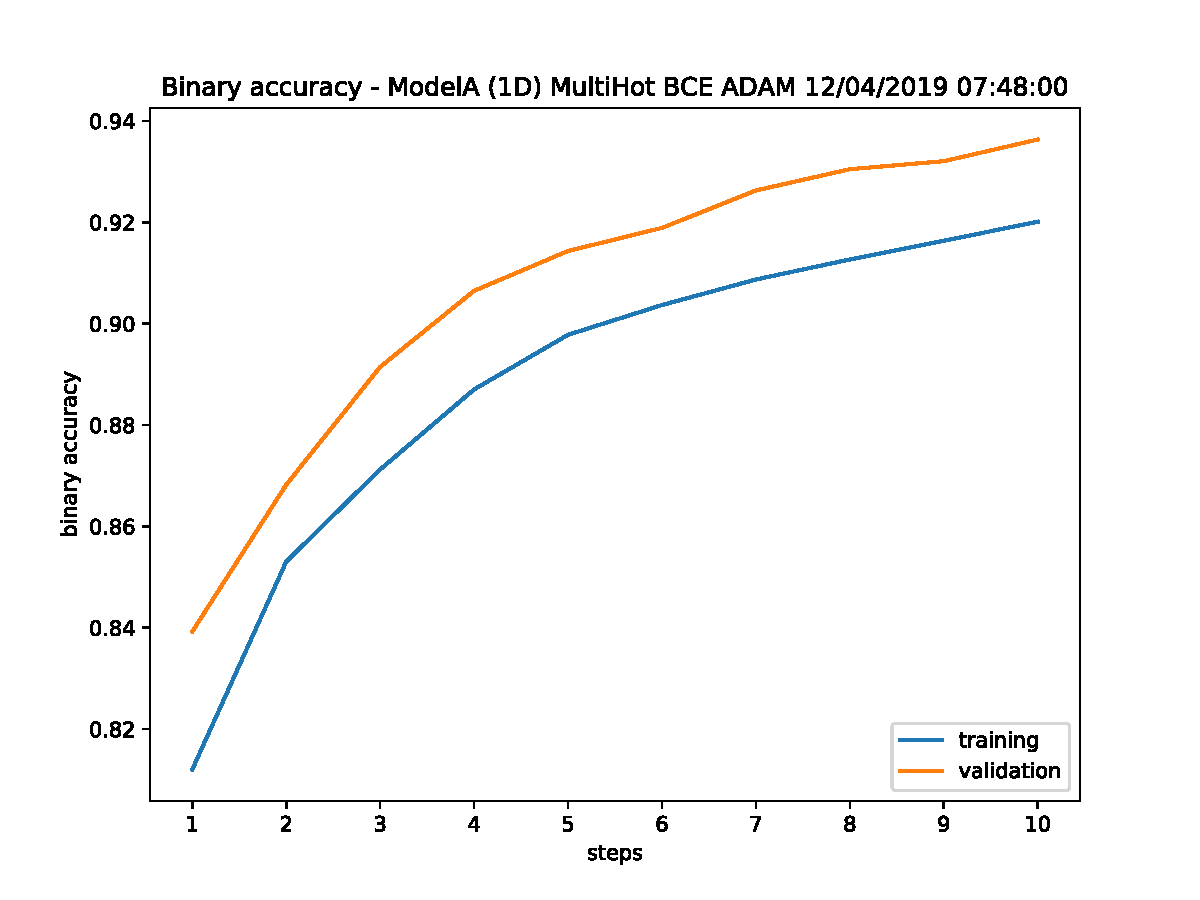
\includegraphics[width=0.48\textwidth]{figures/training_plots/ModelA-(1D)-MultiHot-BCE-ADAM_12-04-2019_07-48-00_binary-accuracy.pdf} \\
                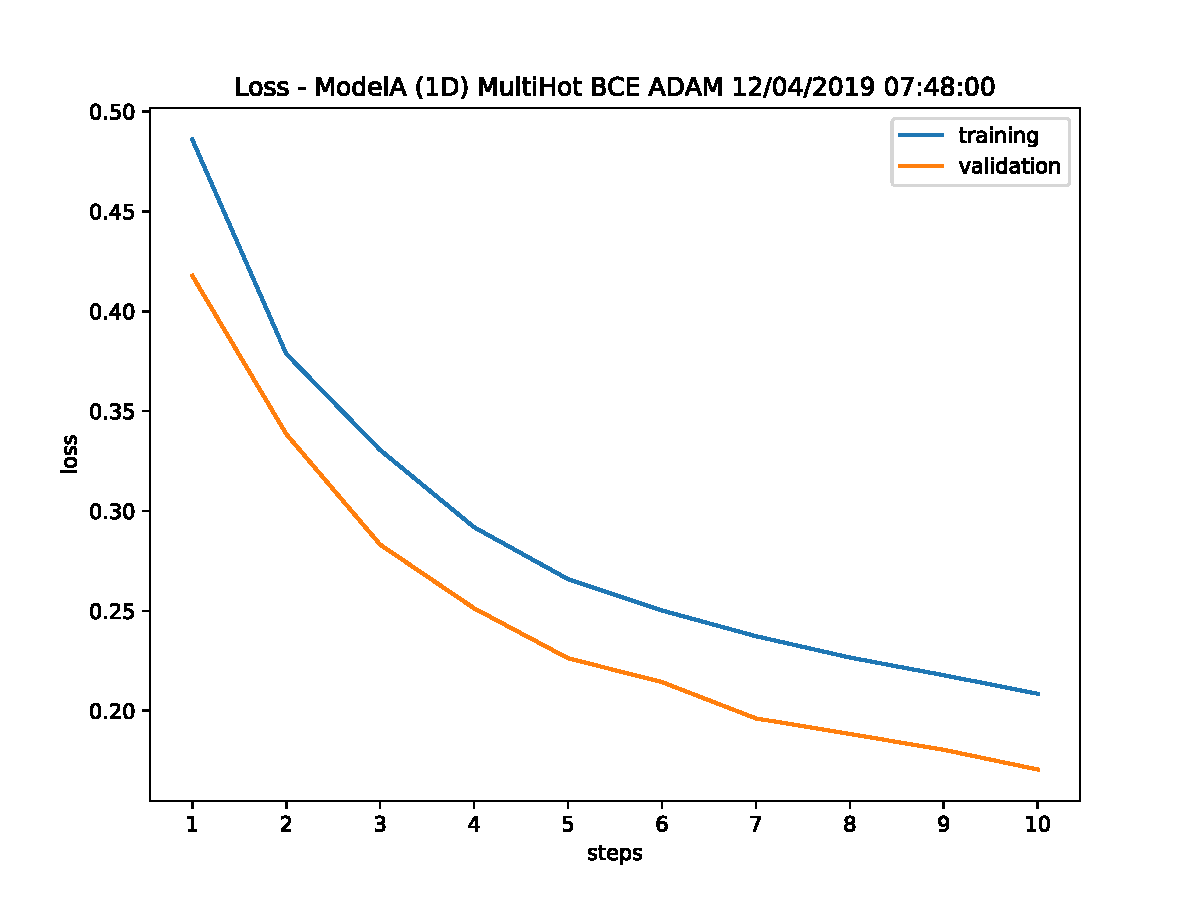
\includegraphics[width=0.48\textwidth]{figures/training_plots/ModelA-(1D)-MultiHot-BCE-ADAM_12-04-2019_07-48-00_loss.pdf} & 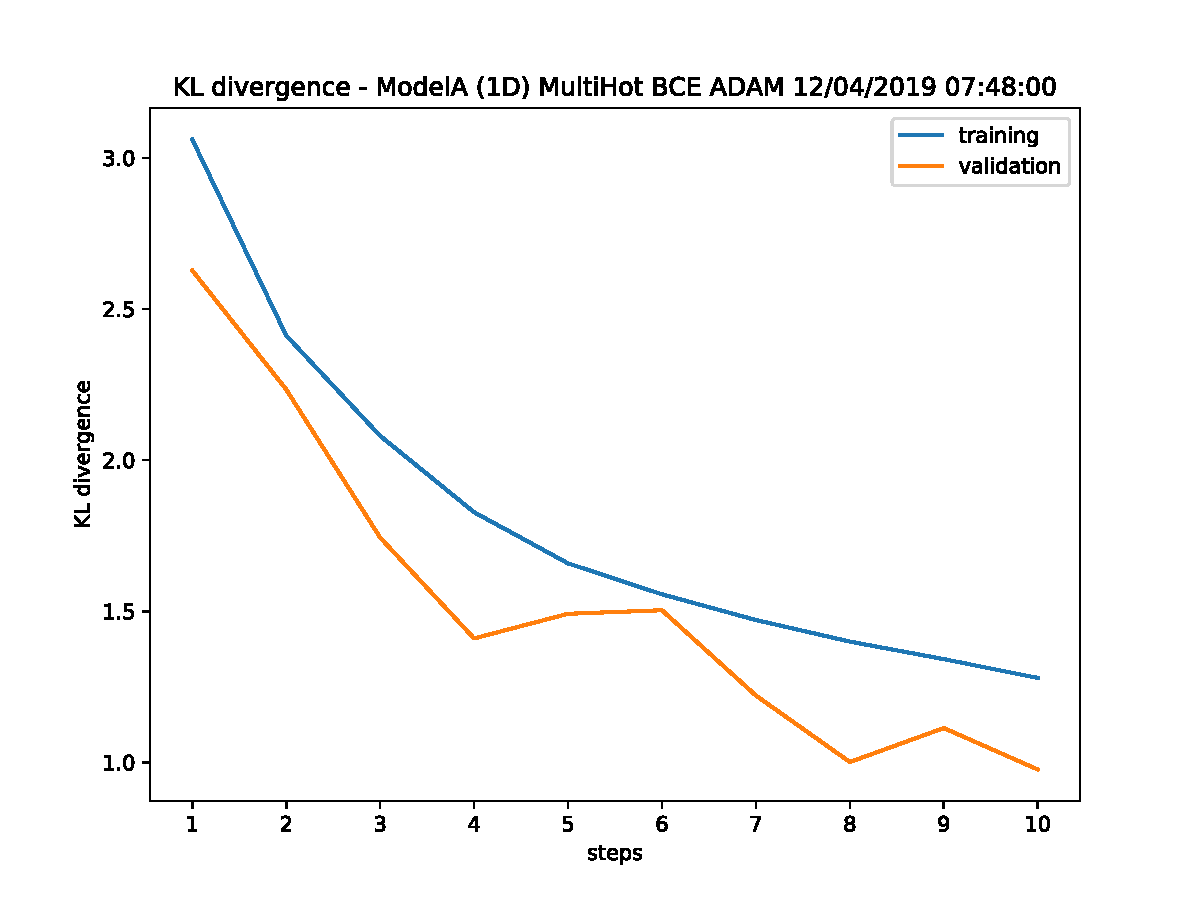
\includegraphics[width=0.48\textwidth]{figures/training_plots/ModelA-(1D)-MultiHot-BCE-ADAM_12-04-2019_07-48-00_KL-divergence.pdf}
            \end{tabular}
            \caption*{Multi-hot encoding, BCE loss}
        \end{figure}
        
        \begin{figure}[H]
            \centering
            \begin{tabular}{cc}
                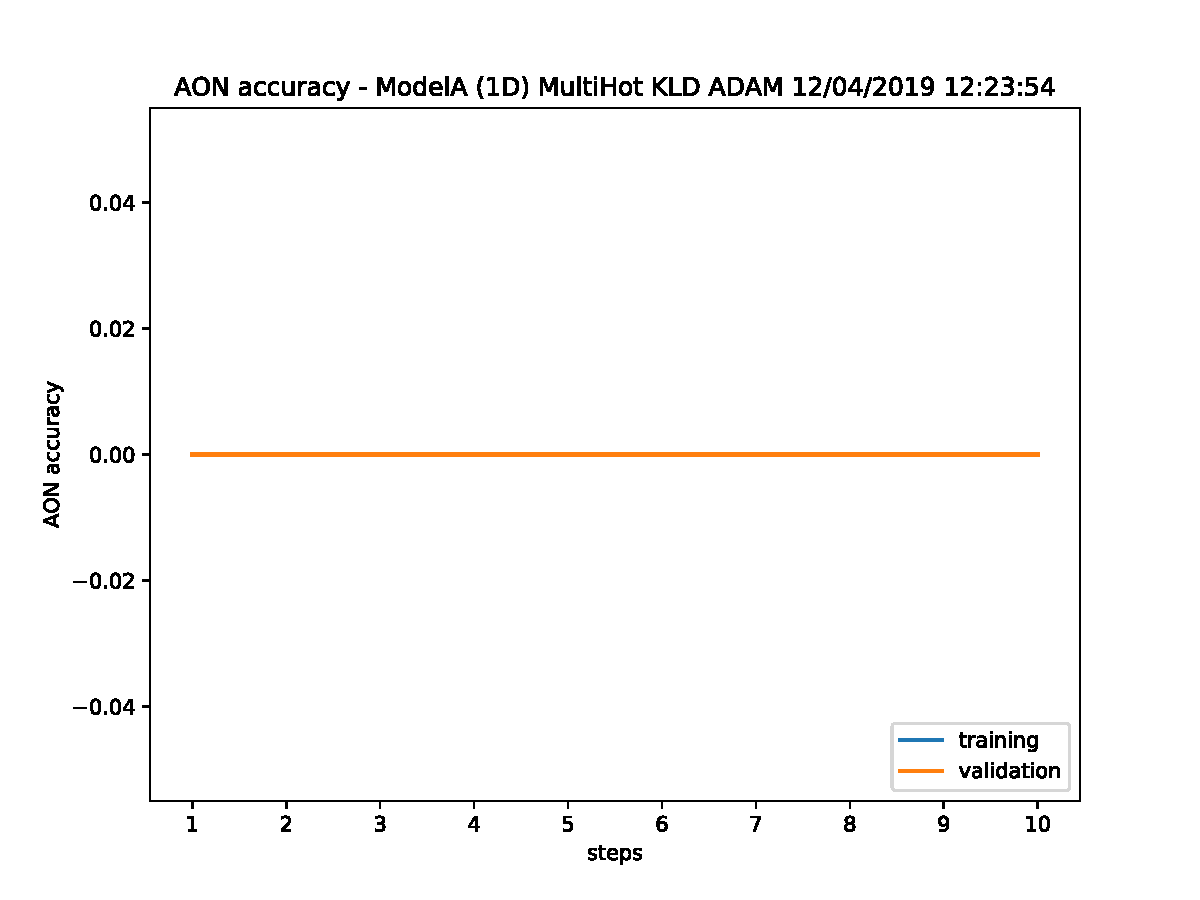
\includegraphics[width=0.48\textwidth]{figures/training_plots/ModelA-(1D)-MultiHot-KLD-ADAM_12-04-2019_12-23-54_AON-accuracy.pdf} & 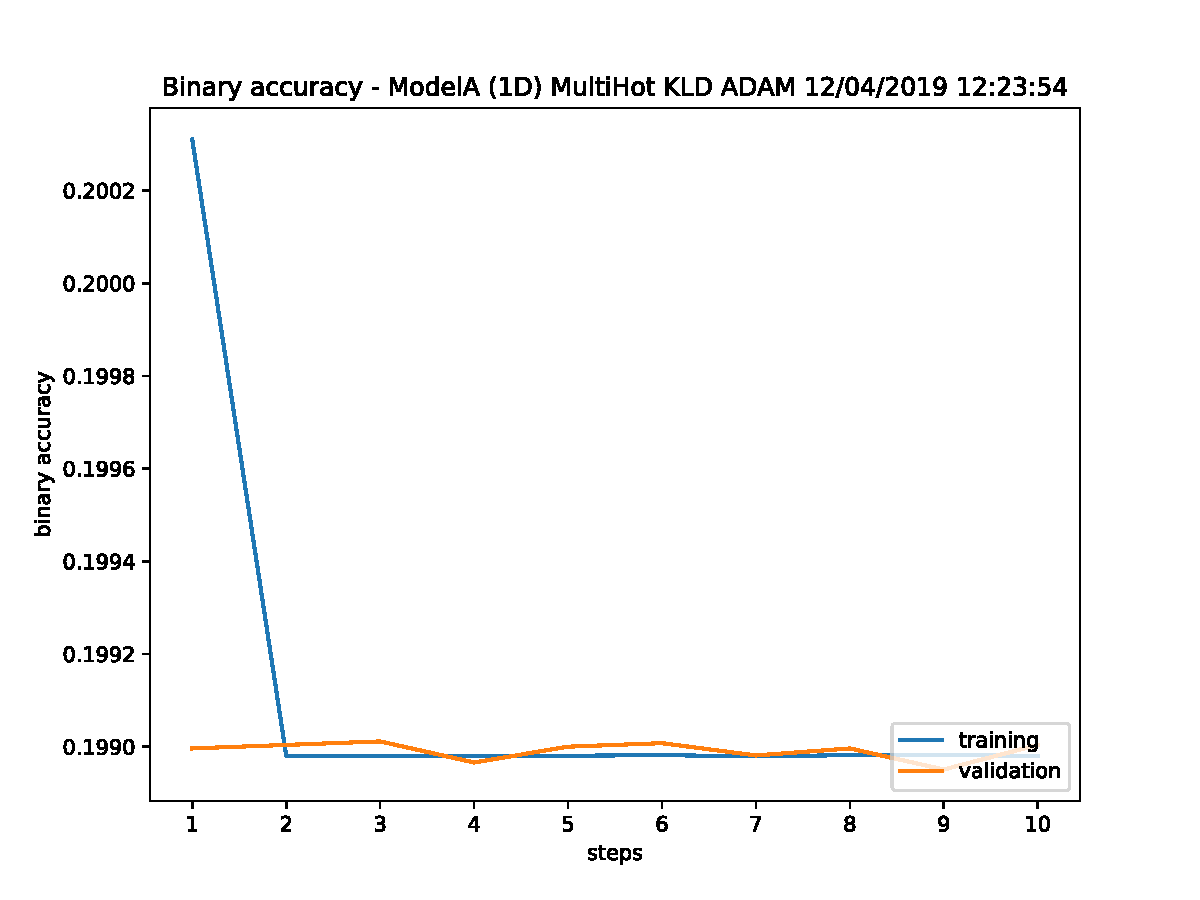
\includegraphics[width=0.48\textwidth]{figures/training_plots/ModelA-(1D)-MultiHot-KLD-ADAM_12-04-2019_12-23-54_binary-accuracy.pdf} \\
                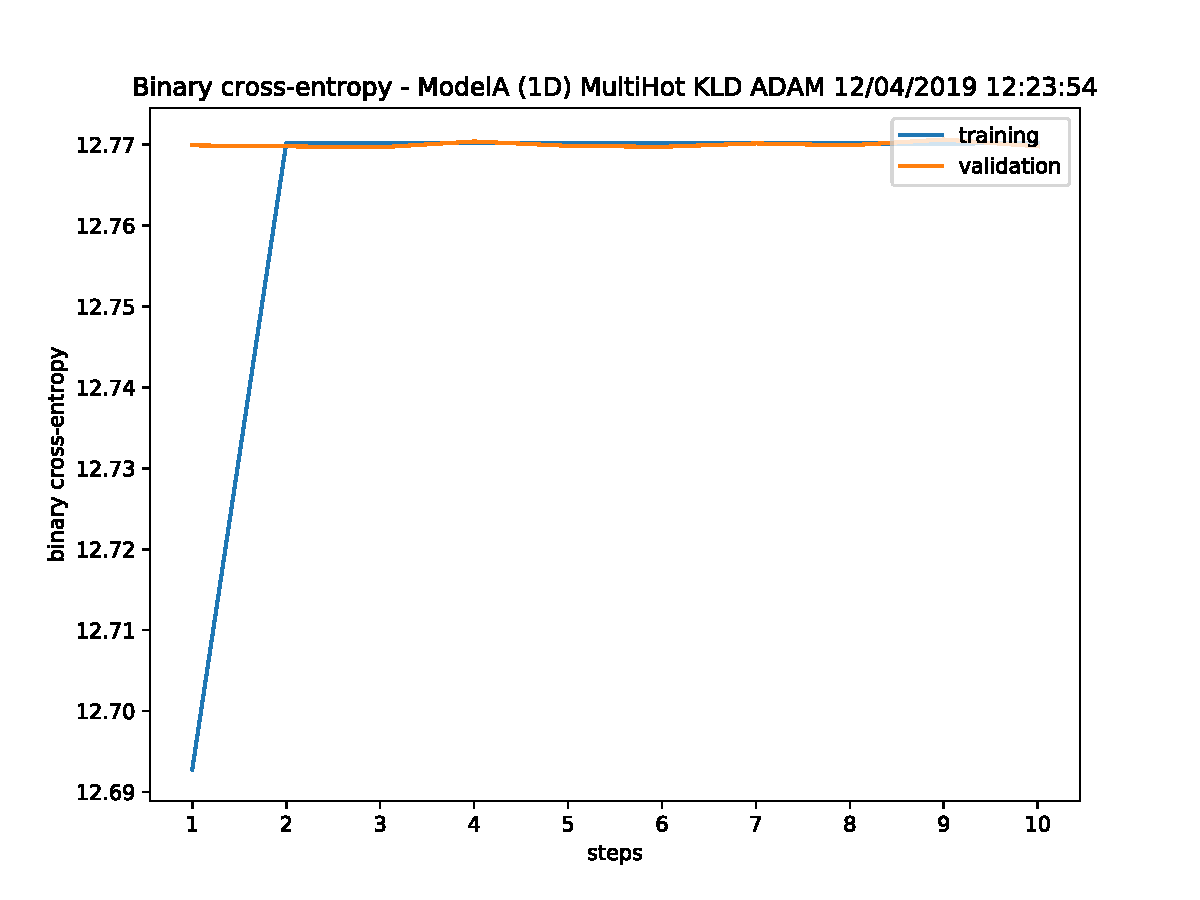
\includegraphics[width=0.48\textwidth]{figures/training_plots/ModelA-(1D)-MultiHot-KLD-ADAM_12-04-2019_12-23-54_binary-cross-entropy.pdf} & 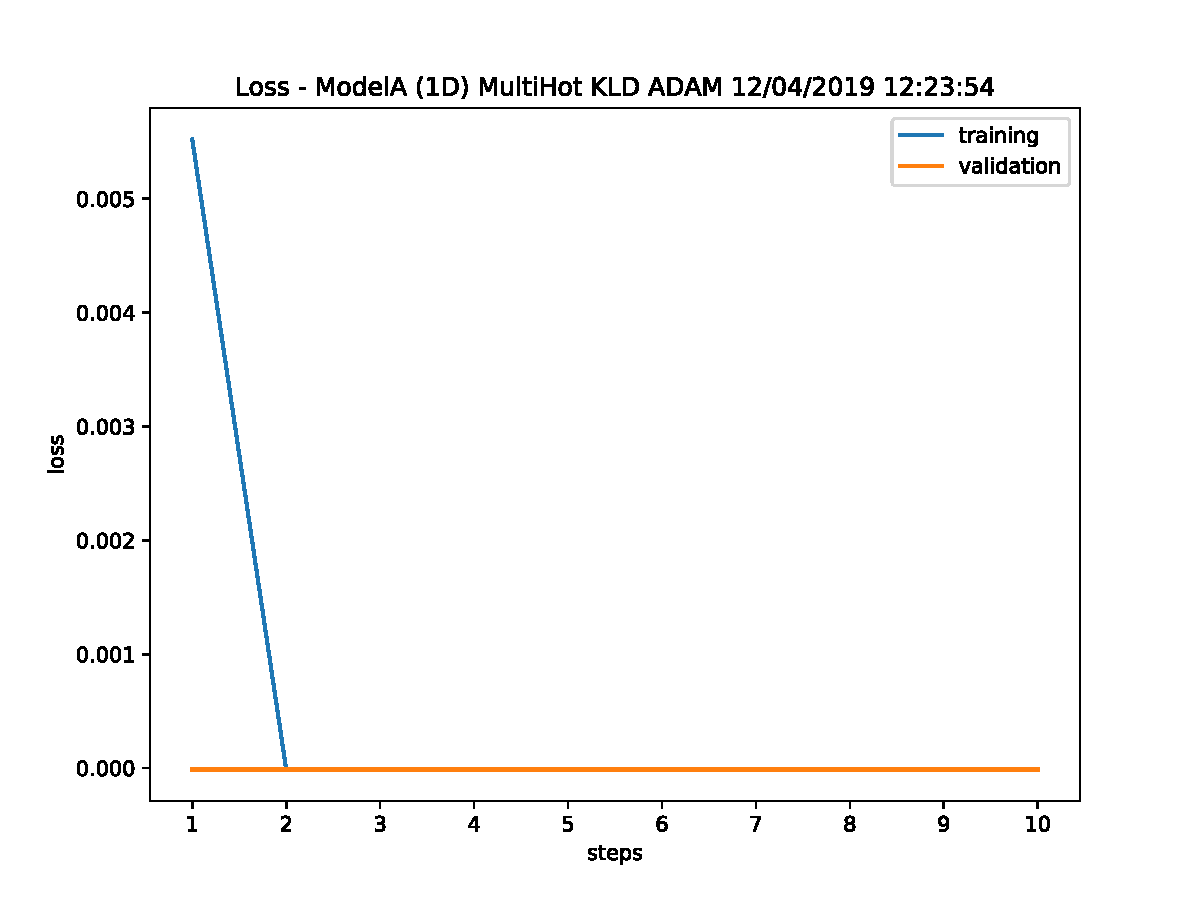
\includegraphics[width=0.48\textwidth]{figures/training_plots/ModelA-(1D)-MultiHot-KLD-ADAM_12-04-2019_12-23-54_loss.pdf}
            \end{tabular}
            \caption*{Multi-hot encoding, KLD loss}
        \end{figure}
        
        \subsection{Model B training metrics}
        \label{app:modelB_training}
        \texttt{Referred to in section \ref{sec:training_analysis_modelB}}
        
        \begin{figure}[H]
            \centering
            \begin{tabular}{cc}
                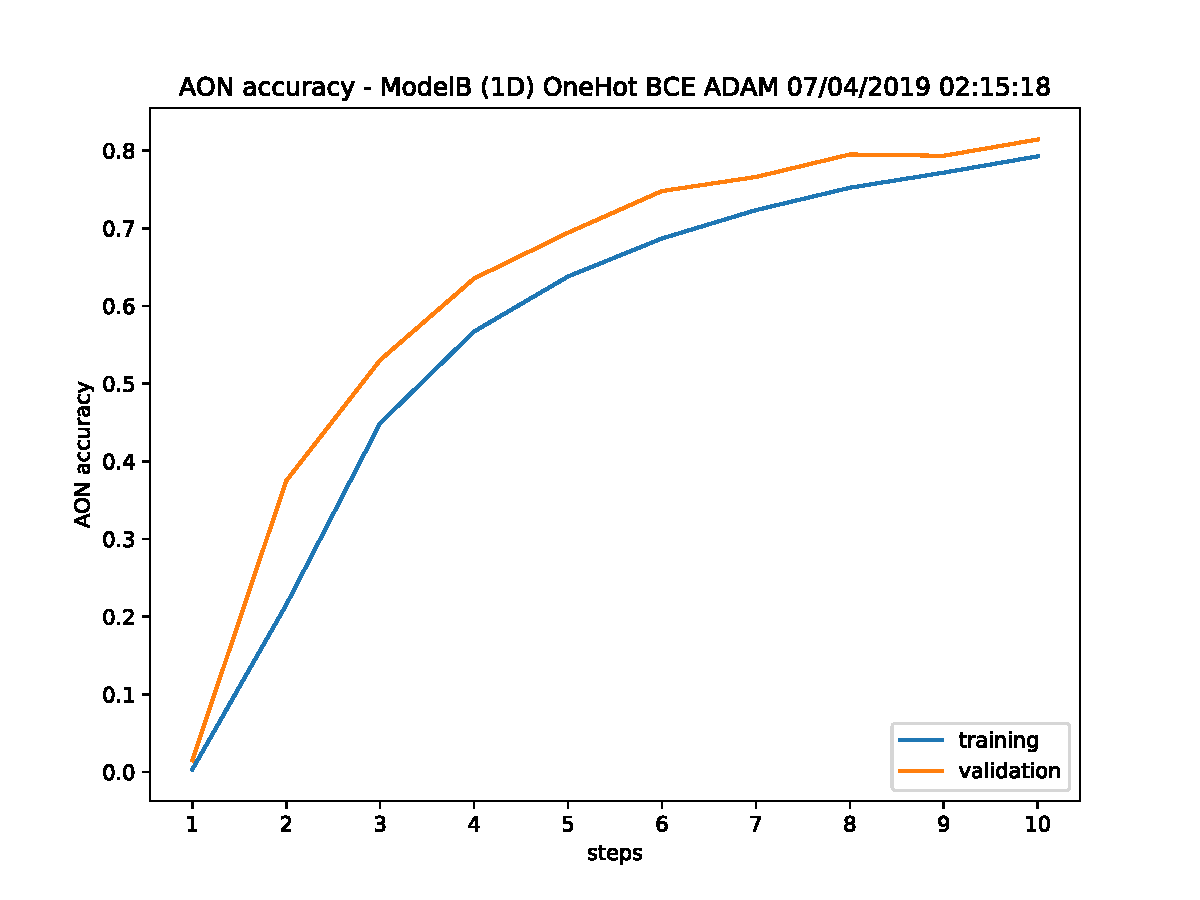
\includegraphics[width=0.45\textwidth]{figures/training_plots/ModelB-(1D)-OneHot-BCE-ADAM_07-04-2019_02-15-18_AON-accuracy.pdf} & 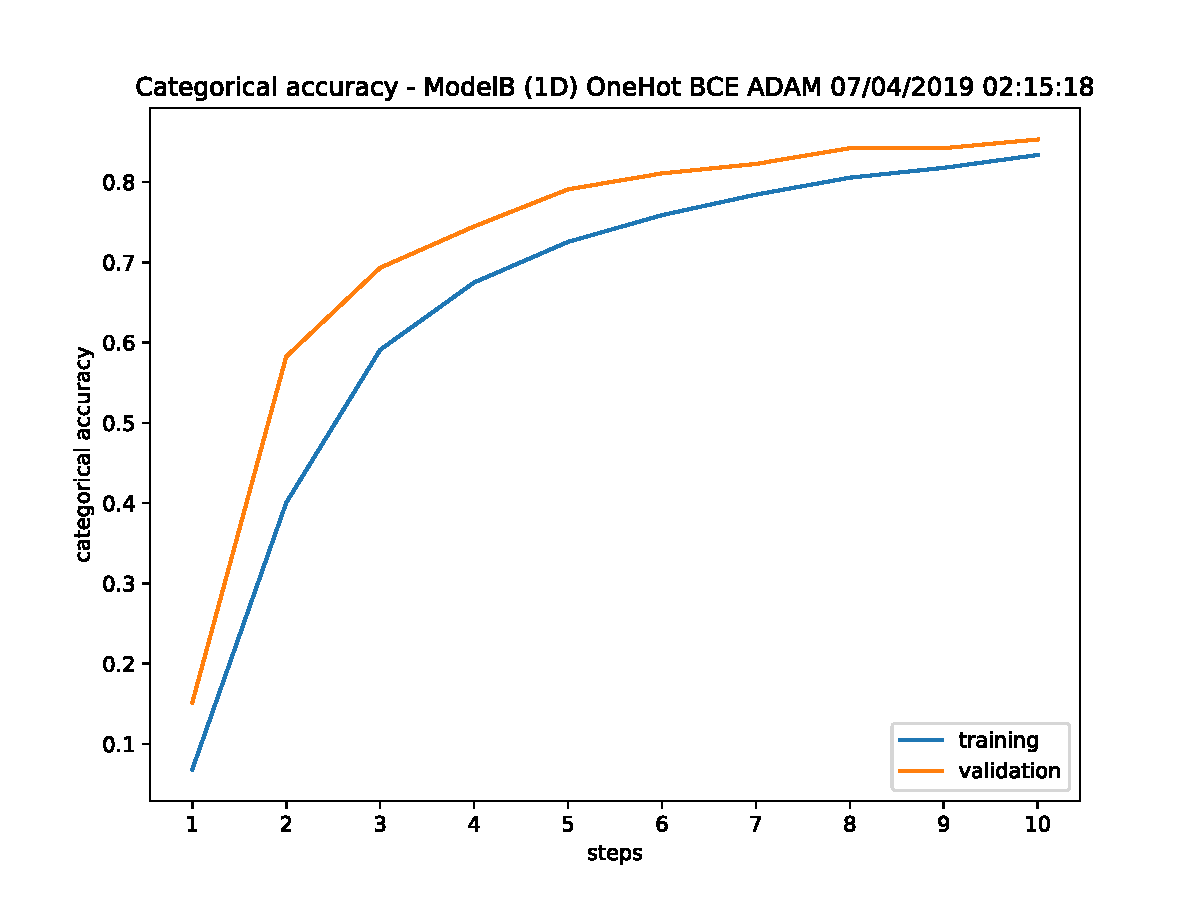
\includegraphics[width=0.45\textwidth]{figures/training_plots/ModelB-(1D)-OneHot-BCE-ADAM_07-04-2019_02-15-18_categorical-accuracy.pdf} \\
                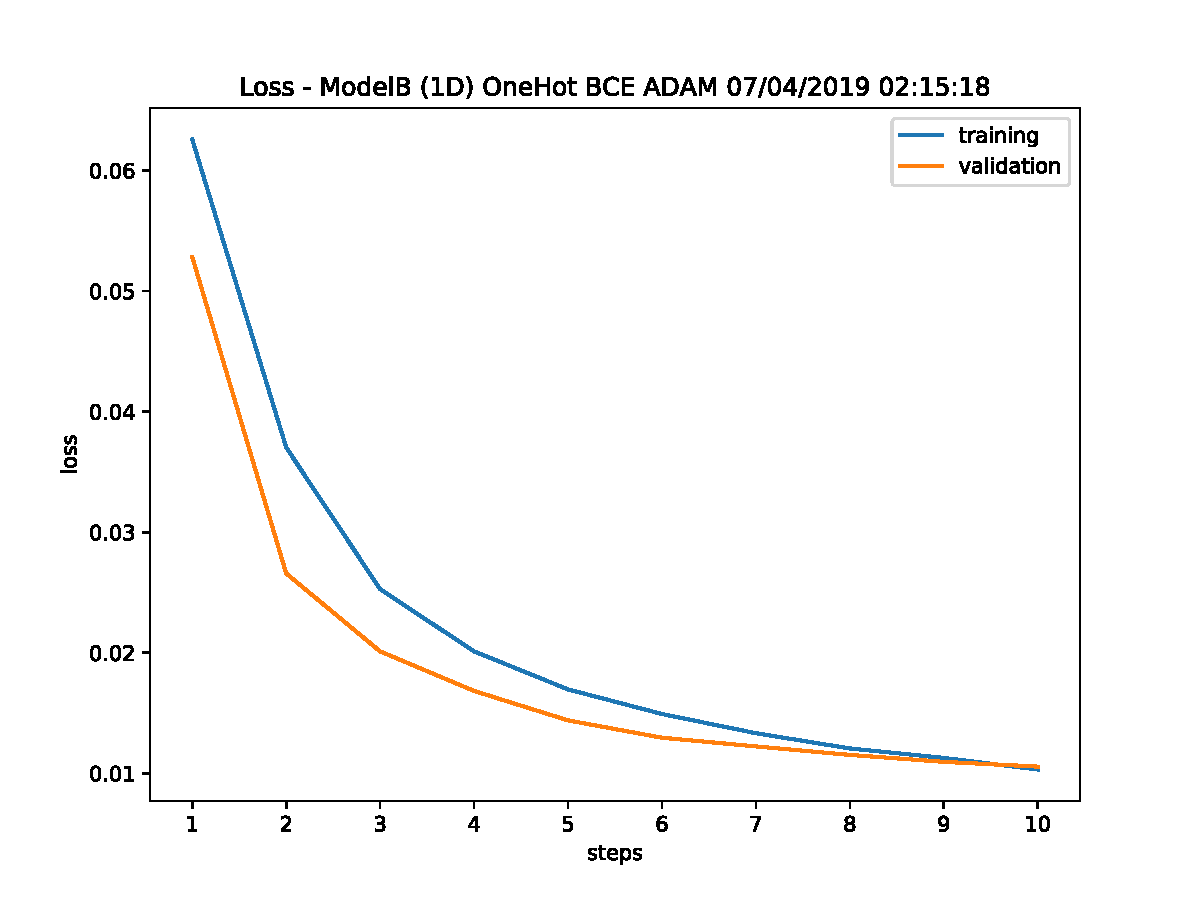
\includegraphics[width=0.45\textwidth]{figures/training_plots/ModelB-(1D)-OneHot-BCE-ADAM_07-04-2019_02-15-18_loss.pdf} & 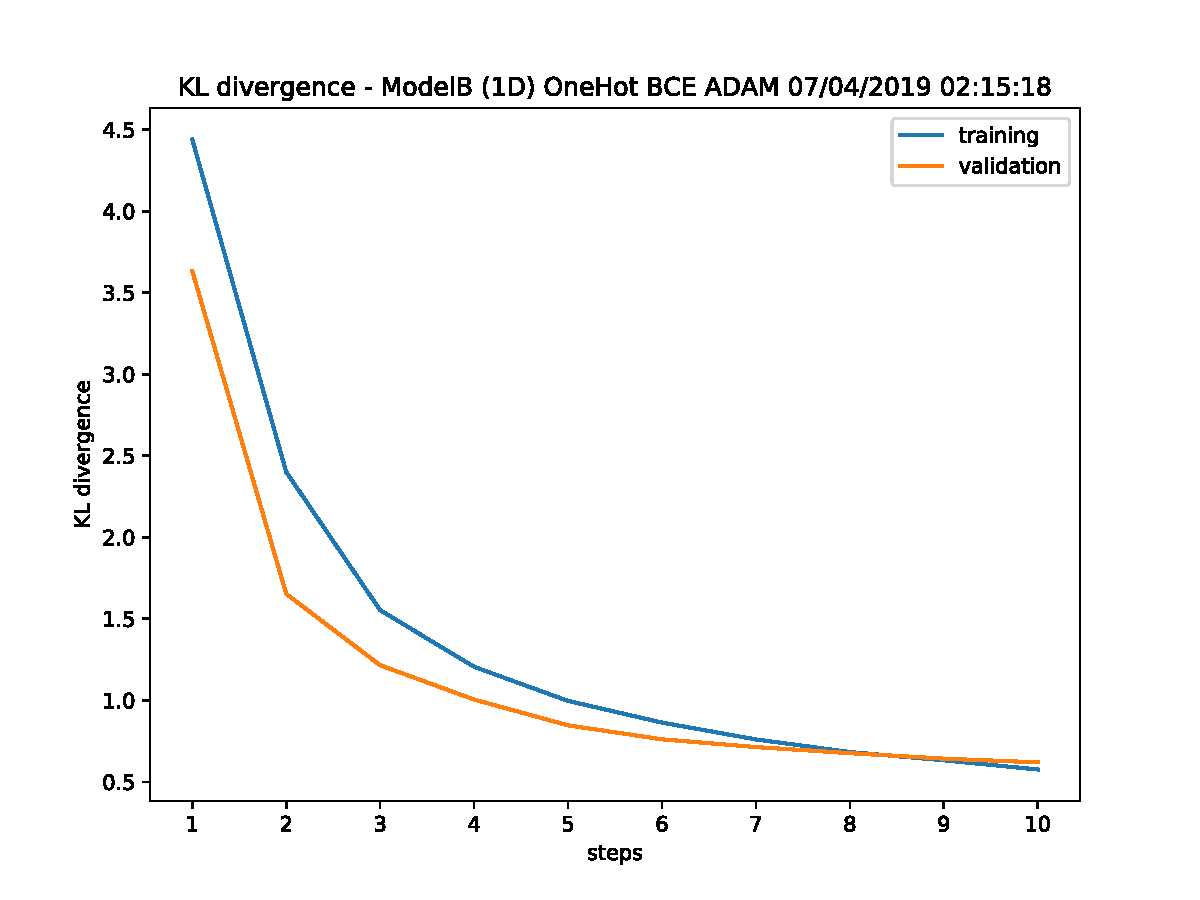
\includegraphics[width=0.45\textwidth]{figures/training_plots/ModelB-(1D)-OneHot-BCE-ADAM_07-04-2019_02-15-18_KL-divergence.pdf}
            \end{tabular}
            \caption*{One-hot encoding, BCE loss}
        \end{figure}
        
        \begin{figure}[H]
            \centering
            \begin{tabular}{cc}
                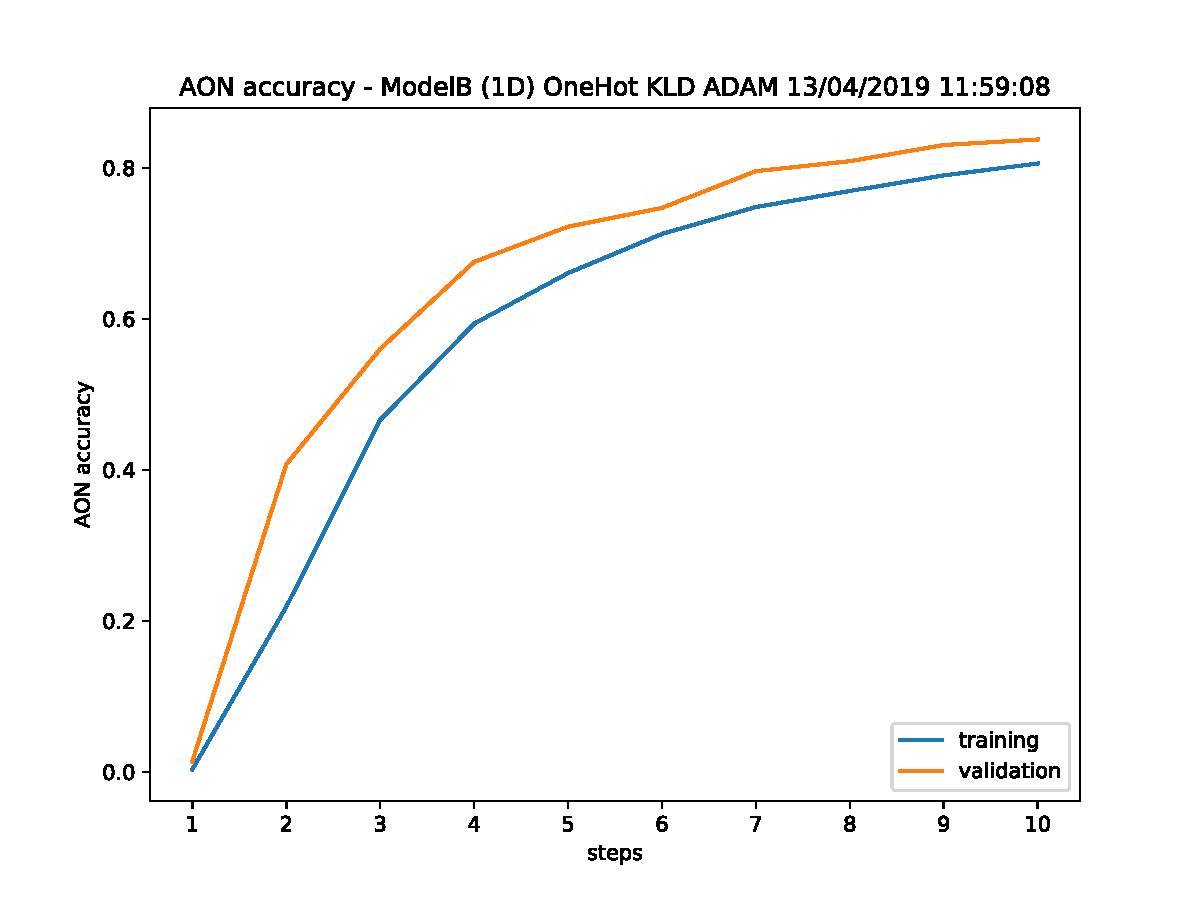
\includegraphics[width=0.45\textwidth]{figures/training_plots/ModelB-(1D)-OneHot-KLD-ADAM_13-04-2019_11-59-08_AON-accuracy.pdf} & 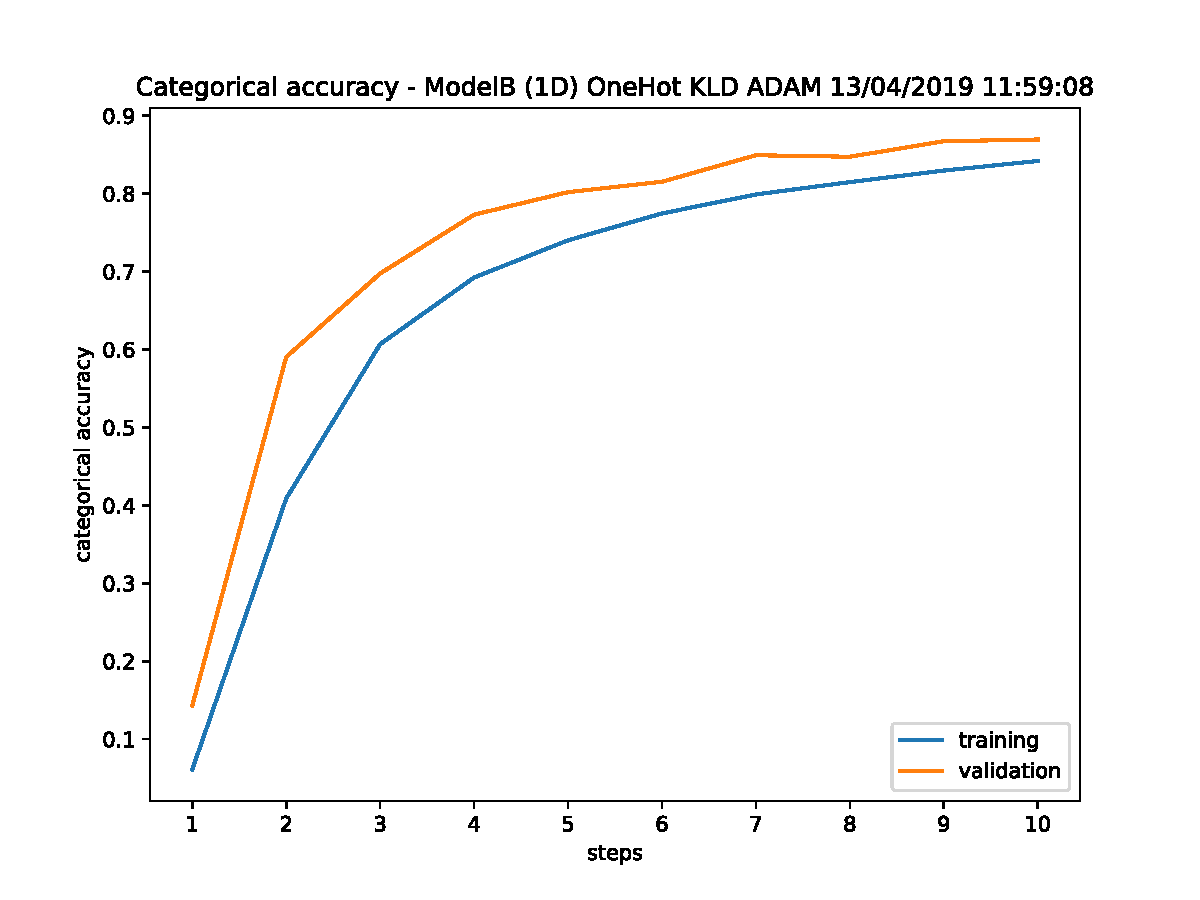
\includegraphics[width=0.45\textwidth]{figures/training_plots/ModelB-(1D)-OneHot-KLD-ADAM_13-04-2019_11-59-08_categorical-accuracy.pdf} \\
                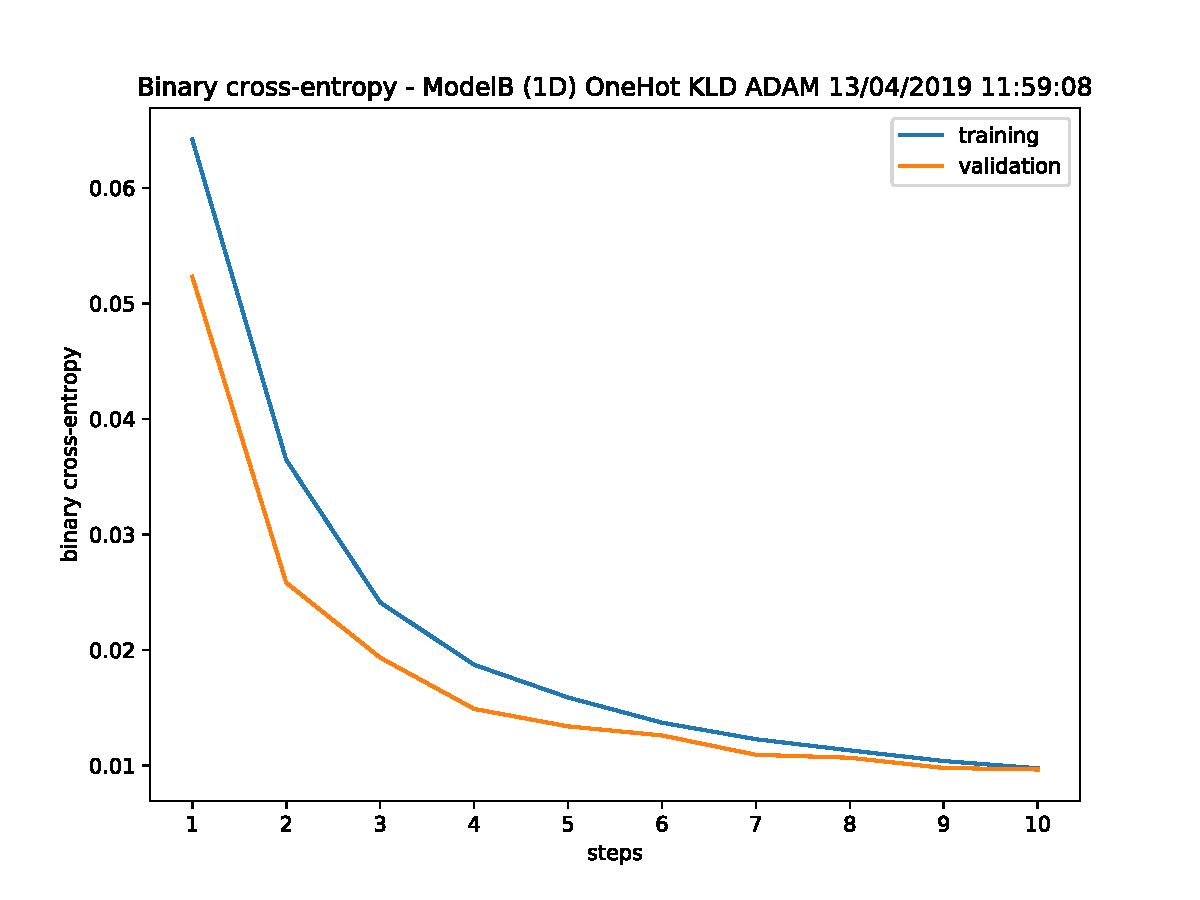
\includegraphics[width=0.45\textwidth]{figures/training_plots/ModelB-(1D)-OneHot-KLD-ADAM_13-04-2019_11-59-08_binary-cross-entropy.pdf} & 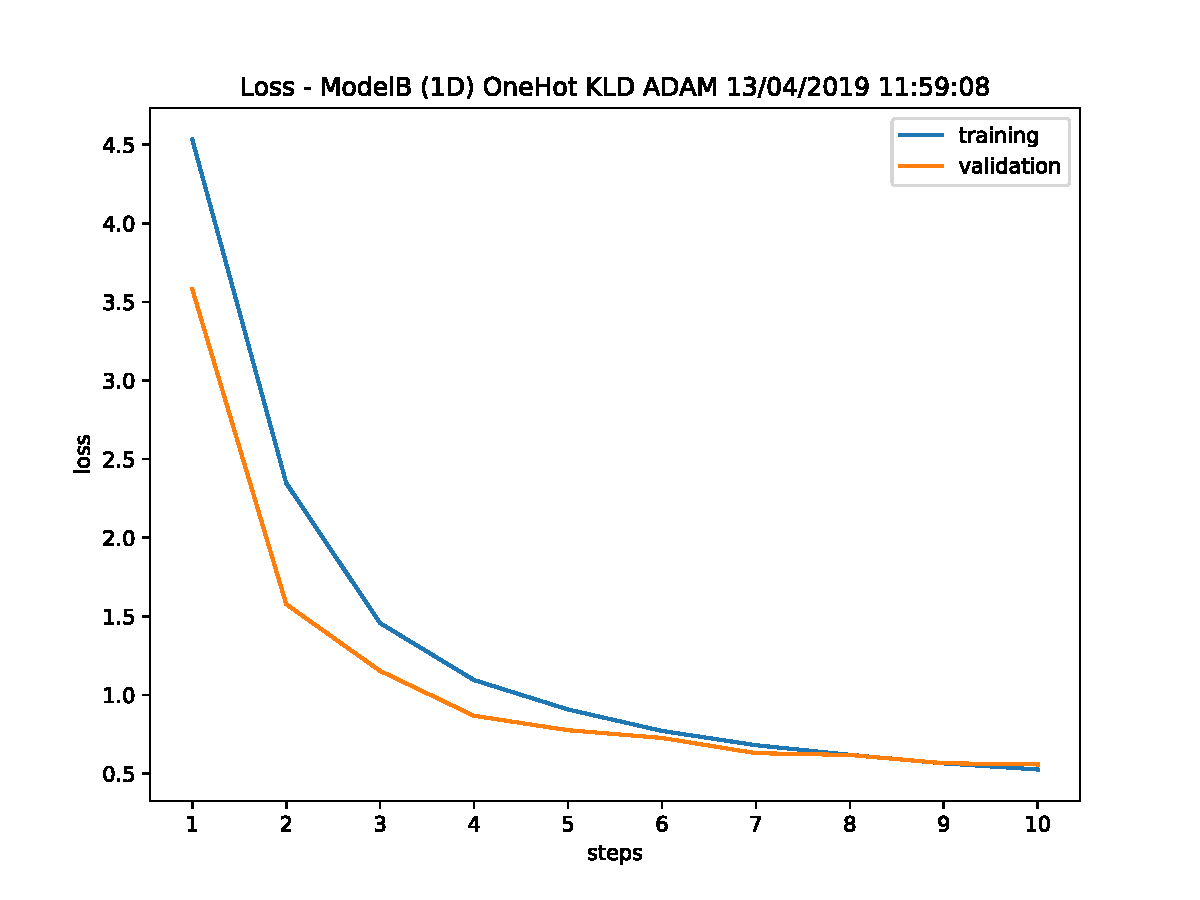
\includegraphics[width=0.45\textwidth]{figures/training_plots/ModelB-(1D)-OneHot-KLD-ADAM_13-04-2019_11-59-08_loss.pdf}
            \end{tabular}
            \caption*{One-hot encoding, KLD loss}
        \end{figure}
        
        \begin{figure}[H]
            \centering
            \begin{tabular}{cc}
                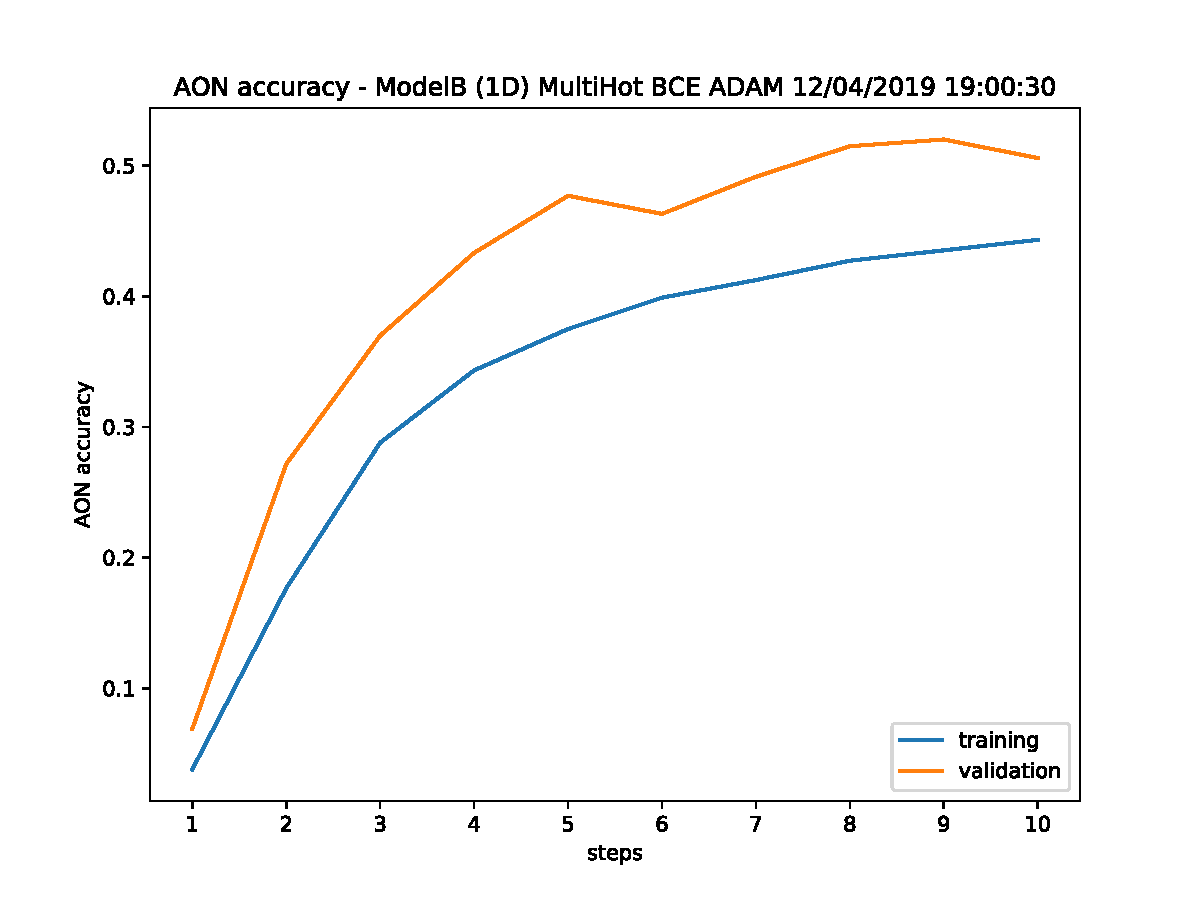
\includegraphics[width=0.48\textwidth]{figures/training_plots/ModelB-(1D)-MultiHot-BCE-ADAM_12-04-2019_19-00-30_AON-accuracy.pdf} & 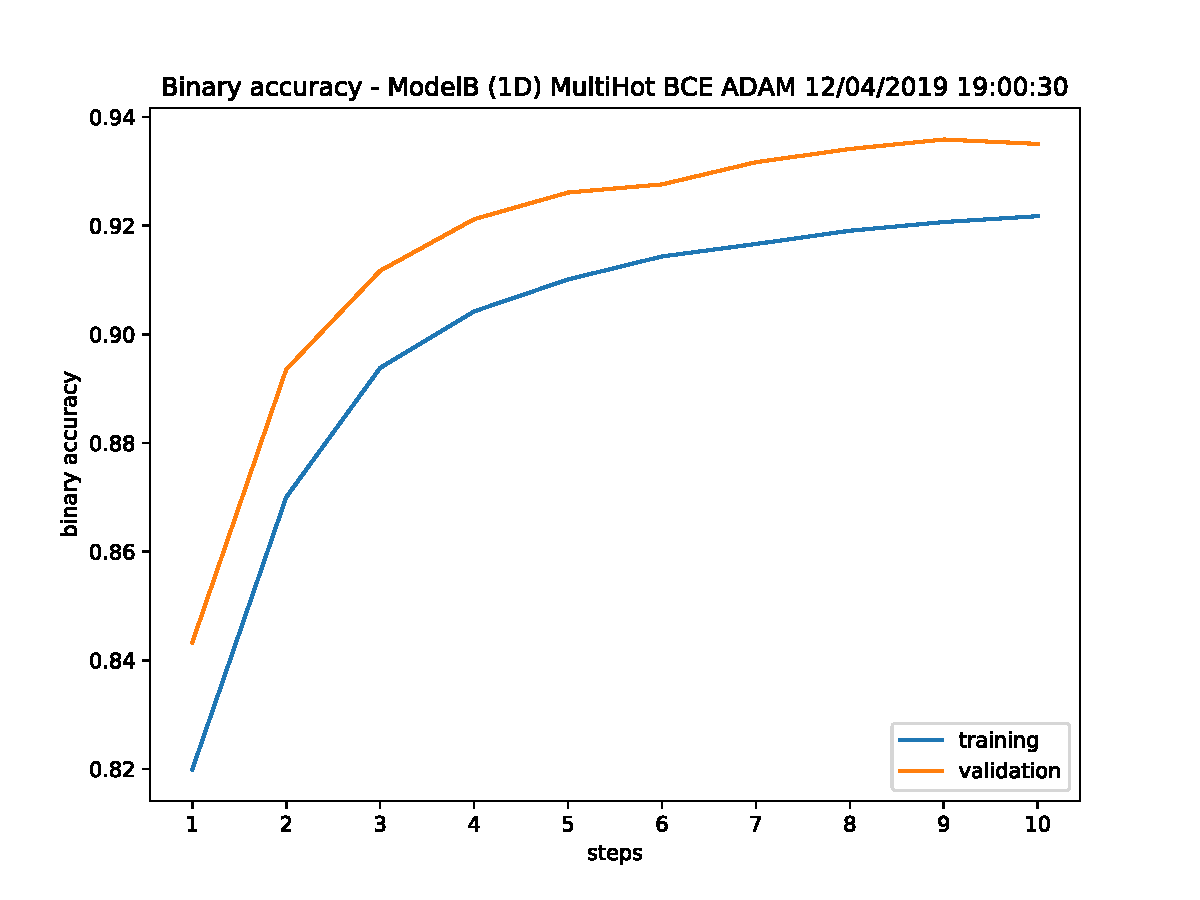
\includegraphics[width=0.48\textwidth]{figures/training_plots/ModelB-(1D)-MultiHot-BCE-ADAM_12-04-2019_19-00-30_binary-accuracy.pdf} \\
                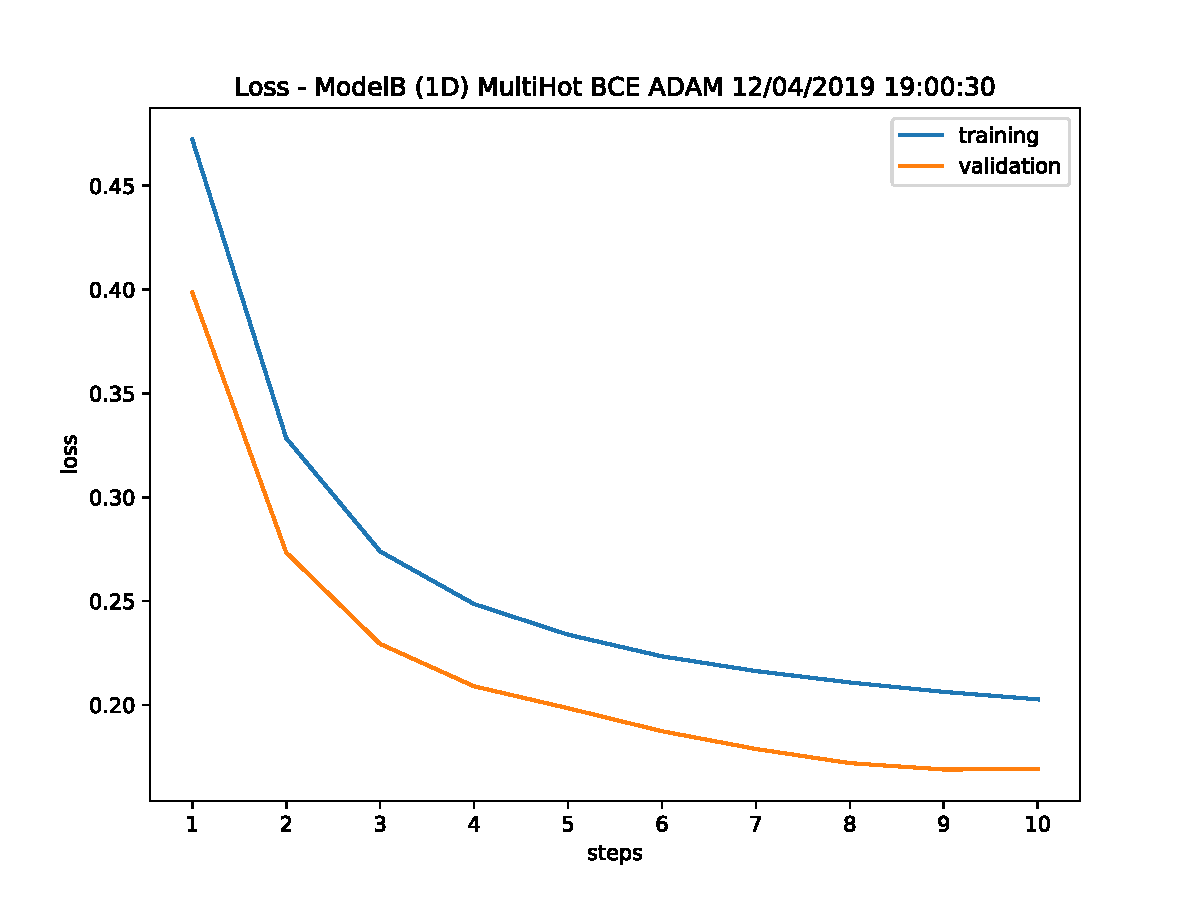
\includegraphics[width=0.48\textwidth]{figures/training_plots/ModelB-(1D)-MultiHot-BCE-ADAM_12-04-2019_19-00-30_loss.pdf} & 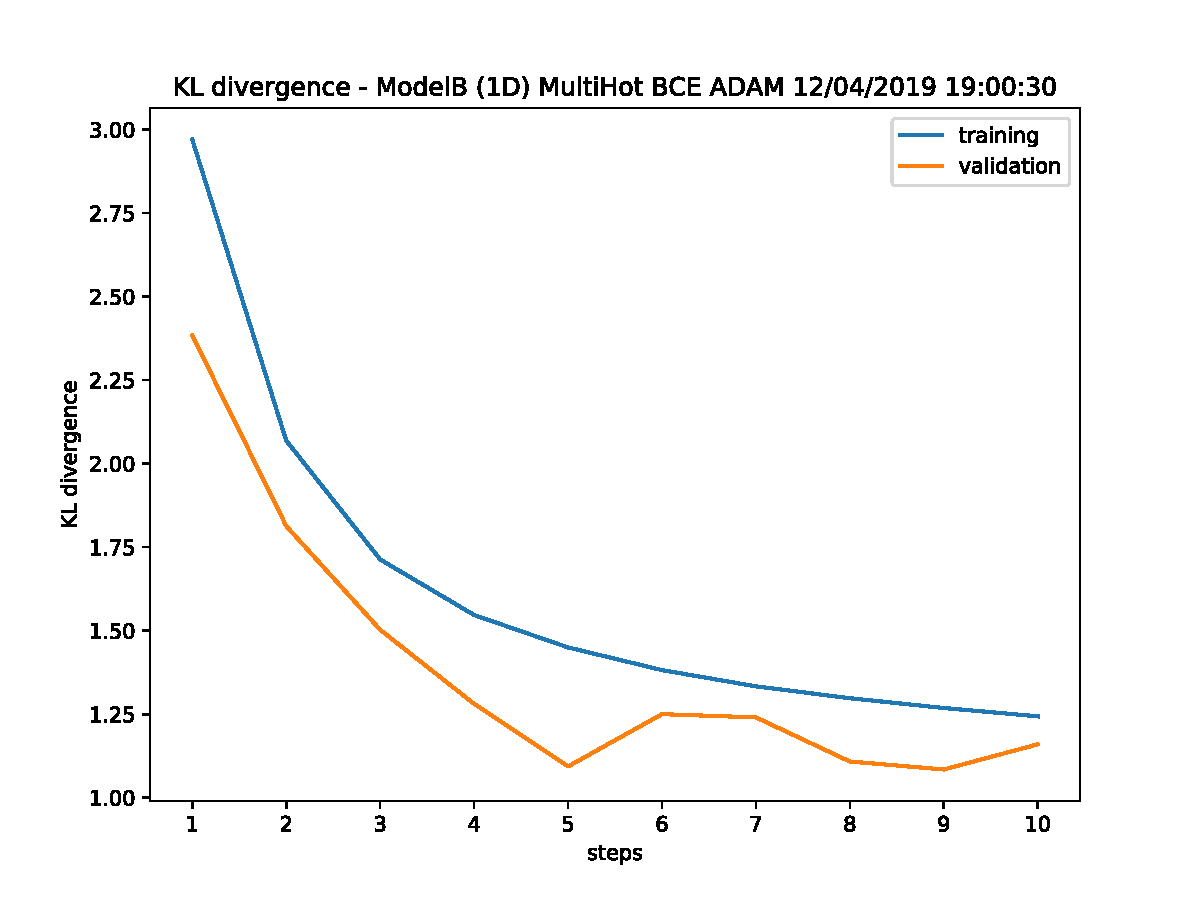
\includegraphics[width=0.48\textwidth]{figures/training_plots/ModelB-(1D)-MultiHot-BCE-ADAM_12-04-2019_19-00-30_KL-divergence.pdf}
            \end{tabular}
            \caption*{Multi-hot encoding, BCE loss}
        \end{figure}
        
        \begin{figure}[H]
            \centering
            \begin{tabular}{cc}
                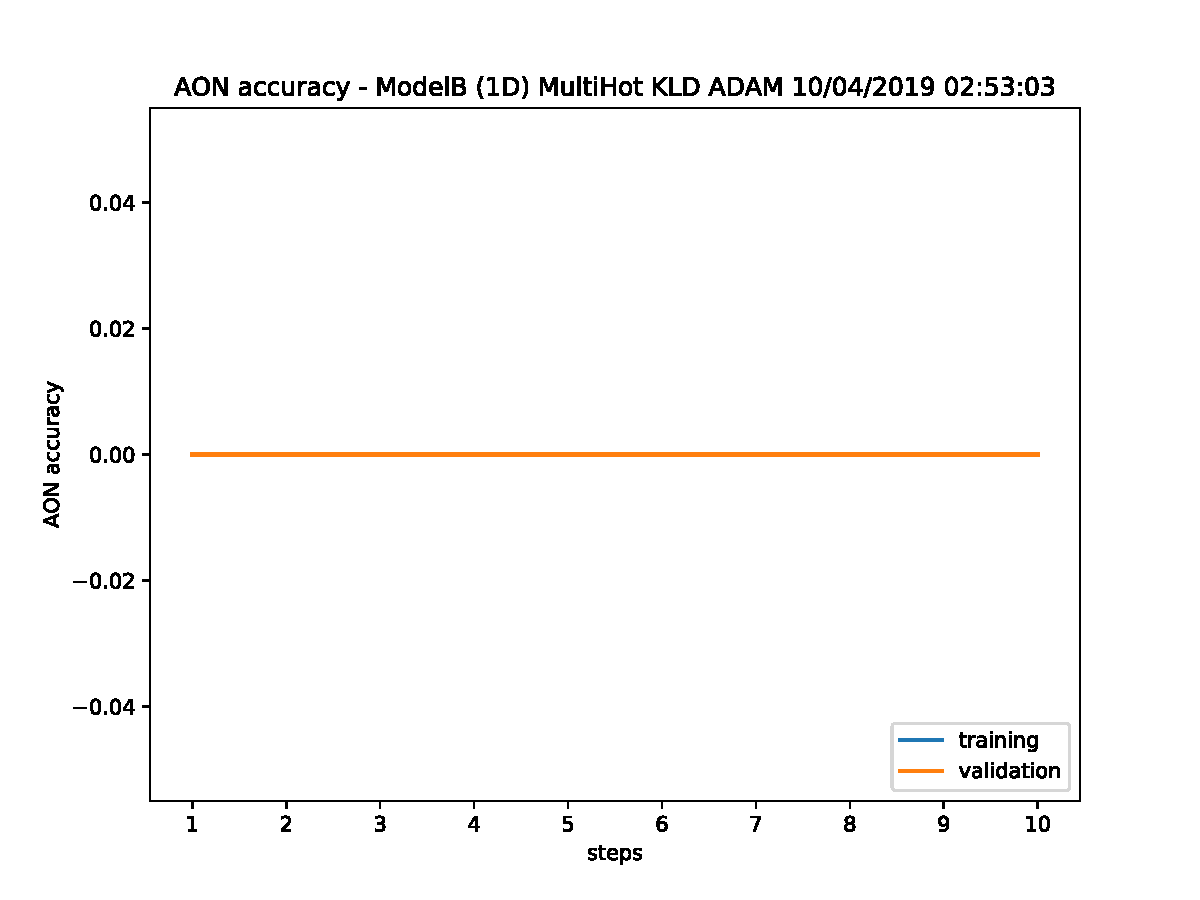
\includegraphics[width=0.48\textwidth]{figures/training_plots/ModelB-(1D)-MultiHot-KLD-ADAM_10-04-2019_02-53-03_AON-accuracy.pdf} & \includegraphics[width=0.48\textwidth]{figures/training_plots/ModelB-(1D)-MultiHot-KLD-ADAM_10-04-2019_02-53-03_binary-accuracy.pdf} \\
                \includegraphics[width=0.48\textwidth]{figures/training_plots/ModelB-(1D)-MultiHot-KLD-ADAM_10-04-2019_02-53-03_binary-cross-entropy.pdf} & \includegraphics[width=0.48\textwidth]{figures/training_plots/ModelB-(1D)-MultiHot-KLD-ADAM_10-04-2019_02-53-03_loss.pdf}
            \end{tabular}
            \caption*{Multi-hot encoding, KLD loss}
        \end{figure}
        
        \subsection{Model C training metrics}
        \label{app:modelC_training}
        \texttt{Referred to in section \ref{sec:training_analysis_modelC}}
        \begin{figure}[H]
            \centering
            \begin{tabular}{cc}
                \includegraphics[width=0.45\textwidth]{figures/training_plots/ModelC-(linear_2D)-OneHot-BCE-ADAM_14-04-2019_02-09-59_AON-accuracy.pdf} & \includegraphics[width=0.45\textwidth]{figures/training_plots/ModelC-(linear_2D)-OneHot-BCE-ADAM_14-04-2019_02-09-59_categorical-accuracy.pdf} \\
                \includegraphics[width=0.45\textwidth]{figures/training_plots/ModelC-(linear_2D)-OneHot-BCE-ADAM_14-04-2019_02-09-59_loss.pdf} & \includegraphics[width=0.45\textwidth]{figures/training_plots/ModelC-(linear_2D)-OneHot-BCE-ADAM_14-04-2019_02-09-59_KL-divergence.pdf}
            \end{tabular}
            \caption*{Linear magnitude, one-hot encoding, BCE loss}
        \end{figure}
        
        \begin{figure}[H]
            \centering
            \begin{tabular}{cc}
                \includegraphics[width=0.45\textwidth]{figures/training_plots/ModelC-(linear_2D)-OneHot-KLD-ADAM_13-04-2019_21-26-52_AON-accuracy.pdf} & \includegraphics[width=0.45\textwidth]{figures/training_plots/ModelC-(linear_2D)-OneHot-KLD-ADAM_13-04-2019_21-26-52_categorical-accuracy.pdf} \\
                \includegraphics[width=0.45\textwidth]{figures/training_plots/ModelC-(linear_2D)-OneHot-KLD-ADAM_13-04-2019_21-26-52_binary-cross-entropy.pdf} & \includegraphics[width=0.45\textwidth]{figures/training_plots/ModelC-(linear_2D)-OneHot-KLD-ADAM_13-04-2019_21-26-52_loss.pdf}
            \end{tabular}
            \caption*{Linear magnitude, one-hot encoding, KLD loss}
        \end{figure}
        
        \begin{figure}[H]
            \centering
            \begin{tabular}{cc}
                \includegraphics[width=0.48\textwidth]{figures/training_plots/ModelC-(linear_2D)-MultiHot-BCE-ADAM_14-04-2019_13-27-14_AON-accuracy.pdf} & \includegraphics[width=0.48\textwidth]{figures/training_plots/ModelC-(linear_2D)-MultiHot-BCE-ADAM_14-04-2019_13-27-14_binary-accuracy.pdf} \\
                \includegraphics[width=0.48\textwidth]{figures/training_plots/ModelC-(linear_2D)-MultiHot-BCE-ADAM_14-04-2019_13-27-14_loss.pdf} & \includegraphics[width=0.48\textwidth]{figures/training_plots/ModelC-(linear_2D)-MultiHot-BCE-ADAM_14-04-2019_13-27-14_KL-divergence.pdf}
            \end{tabular}
            \caption*{Linear magnitude, multi-hot encoding, BCE loss}
        \end{figure}
        
        \begin{figure}[H]
            \centering
            \begin{tabular}{cc}
                \includegraphics[width=0.48\textwidth]{figures/training_plots/ModelC-(linear_2D)-MultiHot-KLD-ADAM_14-04-2019_18-52-21_AON-accuracy.pdf} & \includegraphics[width=0.48\textwidth]{figures/training_plots/ModelC-(linear_2D)-MultiHot-KLD-ADAM_14-04-2019_18-52-21_binary-accuracy.pdf} \\
                \includegraphics[width=0.48\textwidth]{figures/training_plots/ModelC-(linear_2D)-MultiHot-KLD-ADAM_14-04-2019_18-52-21_binary-cross-entropy.pdf} & \includegraphics[width=0.48\textwidth]{figures/training_plots/ModelC-(linear_2D)-MultiHot-KLD-ADAM_14-04-2019_18-52-21_loss.pdf}
            \end{tabular}
            \caption*{Linear magnitude, multi-hot encoding, KLD loss}
        \end{figure}
        
        \begin{figure}[H]
            \centering
            \begin{tabular}{cc}
                \includegraphics[width=0.48\textwidth]{figures/training_plots/ModelC-(log_2D)-OneHot-BCE-ADAM_05-04-2019_20-28-23_AON-accuracy.pdf} & \includegraphics[width=0.48\textwidth]{figures/training_plots/ModelC-(log_2D)-OneHot-BCE-ADAM_05-04-2019_20-28-23_categorical-accuracy.pdf} \\
                \includegraphics[width=0.48\textwidth]{figures/training_plots/ModelC-(log_2D)-OneHot-BCE-ADAM_05-04-2019_20-28-23_loss.pdf} & \includegraphics[width=0.48\textwidth]{figures/training_plots/ModelC-(log_2D)-OneHot-BCE-ADAM_05-04-2019_20-28-23_KL-divergence.pdf}
            \end{tabular}
            \caption*{Log magnitude, one-hot encoding, BCE loss}
        \end{figure}
        
        \begin{figure}[H]
            \centering
            \begin{tabular}{cc}
                \includegraphics[width=0.48\textwidth]{figures/training_plots/ModelC-(log_2D)-OneHot-KLD-ADAM_06-04-2019_08-42-01_AON-accuracy.pdf} & \includegraphics[width=0.48\textwidth]{figures/training_plots/ModelC-(log_2D)-OneHot-KLD-ADAM_06-04-2019_08-42-01_categorical-accuracy.pdf} \\
                \includegraphics[width=0.48\textwidth]{figures/training_plots/ModelC-(log_2D)-OneHot-KLD-ADAM_06-04-2019_08-42-01_binary-cross-entropy.pdf} & \includegraphics[width=0.48\textwidth]{figures/training_plots/ModelC-(log_2D)-OneHot-KLD-ADAM_06-04-2019_08-42-01_loss.pdf}
            \end{tabular}
            \caption*{Log magnitude, one-hot encoding, KLD loss}
        \end{figure}
        
        \begin{figure}[H]
            \centering
            \begin{tabular}{cc}
                \includegraphics[width=0.48\textwidth]{figures/training_plots/ModelC-(log_2D)-MultiHot-BCE-ADAM_13-04-2019_00-21-46_AON-accuracy.pdf} & \includegraphics[width=0.48\textwidth]{figures/training_plots/ModelC-(log_2D)-MultiHot-BCE-ADAM_13-04-2019_00-21-46_binary-accuracy.pdf} \\
                \includegraphics[width=0.48\textwidth]{figures/training_plots/ModelC-(log_2D)-MultiHot-BCE-ADAM_13-04-2019_00-21-46_loss.pdf} & \includegraphics[width=0.48\textwidth]{figures/training_plots/ModelC-(log_2D)-MultiHot-BCE-ADAM_13-04-2019_00-21-46_KL-divergence.pdf}
            \end{tabular}
            \caption*{Log magnitude, multi-hot encoding, BCE loss}
        \end{figure}
        
         \begin{figure}[H]
            \centering
            \begin{tabular}{cc}
                \includegraphics[width=0.48\textwidth]{figures/training_plots/ModelC-(log_2D)-MultiHot-KLD-ADAM_13-04-2019_16-30-38_AON-accuracy.pdf} & \includegraphics[width=0.48\textwidth]{figures/training_plots/ModelC-(log_2D)-MultiHot-KLD-ADAM_13-04-2019_16-30-38_binary-accuracy.pdf} \\
                \includegraphics[width=0.48\textwidth]{figures/training_plots/ModelC-(log_2D)-MultiHot-KLD-ADAM_13-04-2019_16-30-38_binary-cross-entropy.pdf} & \includegraphics[width=0.48\textwidth]{figures/training_plots/ModelC-(log_2D)-MultiHot-KLD-ADAM_13-04-2019_16-30-38_loss.pdf}
            \end{tabular}
            \caption*{Log magnitude, multi-hot encoding, KLD loss}
        \end{figure}
        
    \newpage
    \section{Confusion matrices}
        \subsection{Model A}
        \label{app:modelA_confusion_matrix}
        \texttt{Referred to in section \ref{sec:evaluation_analysis_modelA}}
            \begin{figure}[H]
                \centering
                \includegraphics[width=\textwidth]{figures/confusion_matrices/ModelA-(1D)-OneHot-BCE-ADAM_10-04-2019_10-36-18.pdf}
                \caption*{Model A with one-hot encoding and BCE loss. This model got:  68.62\% $Acc_{AON}$ and left 25.69\% of test data unclassified.}
            \end{figure}
            
            \begin{figure}[H]
                \centering
                \includegraphics[width=\textwidth]{figures/confusion_matrices/ModelA-(1D)-OneHot-KLD-ADAM_10-04-2019_18-45-24.pdf}
                \caption*{Model A with one-hot encoding and KLD loss. This model got:  69.30\% $Acc_{AON}$ and left 24.11\% of test data unclassified.}
            \end{figure}
            
            \begin{figure}[H]
                \centering
                \includegraphics[width=\textwidth]{figures/confusion_matrices/ModelA-(1D)-MultiHot-BCE-ADAM_12-04-2019_07-48-00.pdf}
                \caption*{Model A with multi-hot encoding and BCE loss. This model got:  52.53\% $Acc_{AON}$ and left 19.77\% of test data unclassified.}
            \end{figure}
            
        \newpage
        \subsection{Model B}
        \label{app:modelB_confusion_matrix}
        \texttt{Referred to in section \ref{sec:evaluation_analysis_modelB}}
            \begin{figure}[H]
                \centering
                \includegraphics[width=\textwidth]{figures/confusion_matrices/ModelB-(1D)-OneHot-BCE-ADAM_07-04-2019_02-15-18.pdf}
                \caption*{Model B with one-hot encoding and BCE loss. This model got:  81.53\% $Acc_{AON}$ and left 12.74\% of test data unclassified.}
            \end{figure}
            
            \begin{figure}[H]
                \centering
                \includegraphics[width=\textwidth]{figures/confusion_matrices/ModelB-(1D)-OneHot-KLD-ADAM_13-04-2019_11-59-08.pdf}
                \caption*{Model B with one-hot encoding and KLD loss. This model got:  83.80\% $Acc_{AON}$ and left 12.38\% of test data unclassified.}
            \end{figure}
            
            \begin{figure}[H]
                \centering
                \includegraphics[width=\textwidth]{figures/confusion_matrices/ModelB-(1D)-MultiHot-BCE-ADAM_12-04-2019_19-00-30.pdf}
                \caption*{Model B with multi-hot encoding and BCE loss. This model got: 50.67\% $Acc_{AON}$ and left 21.89\% of test data unclassified.}
            \end{figure}
            
        \newpage
        \subsection{Model C}
        \label{app:modelC_confusion_matrix}
        \texttt{Referred to in section \ref{sec:evaluation_analysis_modelC}}
            \begin{figure}[H]
                \centering
                \includegraphics[width=\textwidth]{figures/confusion_matrices/ModelC-(linear_2D)-OneHot-KLD-ADAM_13-04-2019_21-26-52.pdf}
                \caption*{Model C using linear spectrogram input with one-hot encoding and KLD loss. This model got:  0.69\% $Acc_{AON}$ and left 0.00\% of test data unclassified.}
            \end{figure}
            
            \begin{figure}[H]
                \centering
                \includegraphics[width=\textwidth]{figures/confusion_matrices/ModelC-(linear_2D)-MultiHot-BCE-ADAM_14-04-2019_13-27-14.pdf}
                \caption*{Model C using linear spectrogram input with multi-hot encoding and BCE loss. This model got:  0.93\% $Acc_{AON}$ and left 0.00\% of test data unclassified.}
            \end{figure}
    
            \begin{figure}[H]
                \centering
                \includegraphics[width=\textwidth]{figures/confusion_matrices/ModelC-(log_2D)-OneHot-BCE-ADAM_05-04-2019_20-28-23.pdf}
                \caption*{Model C using log spectrogram input with one-hot encoding and BCE loss. This model got: 62.64\% $Acc_{AON}$ and left 29.06\% of test data unclassified.}
            \end{figure}
            
            \begin{figure}[H]
                \centering
                \includegraphics[width=\textwidth]{figures/confusion_matrices/ModelC-(log_2D)-OneHot-KLD-ADAM_06-04-2019_08-42-01.pdf}
                \caption*{Model C using log spectrogram input with one-hot encoding and KLD loss. This model got: 00.64\% $Acc_{AON}$ and left 0.00\% of test data unclassified.}
            \end{figure}
            
            \begin{figure}[H]
                \centering
                \includegraphics[width=\textwidth]{figures/confusion_matrices/ModelC-(log_2D)-MultiHot-BCE-ADAM_13-04-2019_00-21-46.pdf}
                \caption*{Model C using log spectrogram input with multi-hot encoding and BCE loss. This model got: 46.91\% $Acc_{AON}$ and left 10.67\% of test data unclassified.}
            \end{figure}
    
\end{appendices}

\end{document}